\documentclass[11pt]{article}                                    % Documento de artículo, tamaño de fuente 11pt
\usepackage[spanish]{babel}                                      % Idioma español
\usepackage[a4paper,margin=2.5cm]{geometry}                      % Márgenes
\usepackage{parskip,mlmodern,charter}                                     % Espaciado entre párrafos y fuente
\usepackage{mathtools,amssymb}                                   % Matemáticas avanzadas
\usepackage[output-decimal-marker={,}]{siunitx}                  % Unidades SI
\usepackage{graphicx,subcaption,booktabs,multirow,float}         % Imágenes y tablas
\usepackage{algorithmicx}                                        % Pseudocódigo
\usepackage{xcolor}                                              % Definición de colores
\usepackage{fancyhdr,lastpage}                                   % Encabezados y pies de página
\usepackage[numbers,square,sort]{natbib}                         % Bibliografía con estilo numérico
\usepackage[colorlinks=true, linkcolor=black, urlcolor=magenta, 
            citecolor=orange, anchorcolor=blue]{hyperref}        % Hipervínculos
\usepackage{microtype}                                           % Mejoras tipográficas

\graphicspath{{Imagenes/}}

\title{\textbf{Control de Accionamientos y Automatización de Grúa
Portacontenedores de Muelle tipo Pórtico} \\ \Large{Proyecto Global Integrador} \\ \texttt{VERSIÓN EXPERIMENTAL}}

\author{Aleo Rodrigo \\ Pucciarelli Nahuel \\ \\ AUTÓMATAS Y CONTROL DISCRETO \\ Profesor Ing. Julián Gabriel
\\ \\ Universidad Nacional de Cuyo \\ Mendoza, Argentina}

\date{2026}

\begin{document}

 % Configuración de encabezados y pies de página
\pagestyle{fancy}
\fancyhf{}
\fancyfoot[R]{\thepage}
\renewcommand{\headrulewidth}{0pt} 
\urlstyle{same} 

\maketitle

\begin{abstract}
    En este trabajo se realizará el desarrollo e implementación de un Sistema Híbrido de Control y Protección con Operación Semi-Automática coordinada para una Grúa Portacontenedores Portuaria de Muelle tipo Pórtico, para carga y descarga de contenedores en grandes barcos de transporte marítimo.

    El sistema híbrido de control y protección incluirá 3 niveles jerárquicos:
    \begin{itemize}
        \item Nivel 2 - Control Regulatorio: estados continuos, muestreados en tiempo discretizado (Sampled CTDS).
        \item Nivel 1 - Control Supervisor: autómata, estados discretos activados por eventos (DEDS).
        \item Nivel 0 - Protección: en espera; actúa en situación de emergencia, lleva el sistema a estado seguro.
    \end{itemize}
\end{abstract}

\newpage
\tableofcontents

\newpage
\section{Modelado de la Planta}
Este proyecto considera el control de accionamientos eléctricos y operación semi-automática coordinada de los dos movimientos principales continuos y simultáneos de la grúa en un plano vertical (2D): traslación horizontal del carro (Trolley) sobre las vigas principal y móvil (paralelo al eje $x$); e Izaje/descenso, o traslación vertical, de la carga (Hoist) bajo la posición del carro (paralelo al eje $y$).

Ambos movimientos son impulsados mediante cables de acero (wireropes) desde mecanismos rotativos con tambores, cajas de engranajes, frenos mecánicos y motores eléctricos, ubicados en una Casa de Máquinas (Machinery House) fija, con sus correspondientes accionamientos electrónicos de velocidad variable; dichos movimientos tienen \textit{restricciones de operación}: posiciones límite de recorrido, velocidades máximas y aceleraciones máximas. Están \textit{acoplados entre sí por la carga} (headblock/spreader con o sin container), que se balancea suspendida del carro que la traslada mediante los cables de izaje.
\begin{figure}[H]
    \centering
    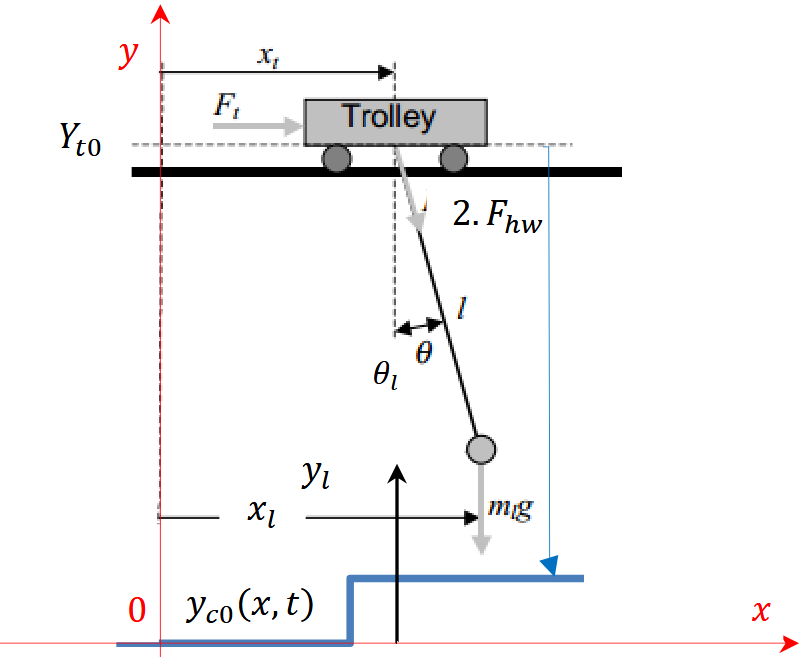
\includegraphics[width=0.7\textwidth]{model_simple.png}
    \caption{Diagrama básico del modelo.}
    \label{fig:basic_model}
\end{figure}

\subsubsection*{Hipótesis simplificativas}
Para el modelado dinámico de los movimientos de la grúa, se consideran las siguientes hipótesis simplificativas:
\begin{itemize}
    \item \textit{Estructura:} Se asume totalmente rígida; se desprecian las deformaciones y vibraciones de las vigas y el pórtico.
    \item \textit{Mecanismo de carro:} Se modela como una transmisión rígida accionada por un cable equivalente siempre en tensión, considerando su elasticidad longitudinal y amortiguamiento.
    \item \textit{Sistema de izaje:} Se simplifica a un sistema equivalente (un solo motor/tambor). El cable se considera de masa despreciable y comportamiento elástico solo a tracción (no soporta compresión).
    \item \textit{Carga:} Se modela como una masa puntual concentrada en la base del spreader, con 2 grados de libertad en el plano vertical (2D).
    \item \textit{Efectos externos:} Solo se consideran la gravedad y las fuerzas de contacto vertical (modelo elástico lineal). Se desprecia la resistencia aerodinámica frontal al viento de la carga y del carro en movimiento.
\end{itemize}

\subsection{Subsistema del Carro (Trolley)}
El sistema de traslación del carro se modela como un sistema electromecánico de dos masas (inercia rotacional del accionamiento y masa traslacional del carro) acopladas mediante un elemento flexible (cable de acero). A continuación, se presentan las ecuaciones fundamentales y su desarrollo para la simulación.
\begin{figure}[H]
    \centering
    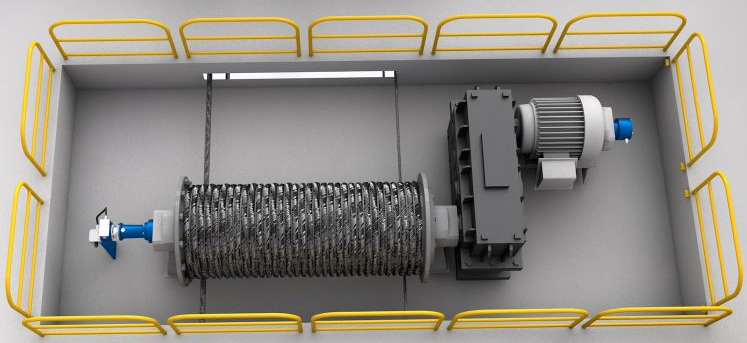
\includegraphics[width=1\textwidth]{trolley.png}
    \caption{Diagrama del subsistema del carro (tambor-motor) (Trolley).}
    \label{fig:trolley}
\end{figure}
\subsubsection{Dinámica del Carro}
Aplicando la segunda ley de Newton al movimiento horizontal del carro, se tiene:
\begin{equation} \label{eq:carro_newton}
    M_t \, \frac{d \, v_t(t)}{dt} = F_{tw}(t) - b_t \, v_t(t) + F_{coupling}(t)
\end{equation}
Donde:
\begin{itemize}
    \item $M_t$: Masa del carro.
    \item $F_{tw}(t)$: Fuerza de tracción ejercida por el cable.
    \item $b_t$: Coeficiente de fricción viscosa del carro sobre los rieles.
    \item $F_{coupling}(t) = 2 F_{hw} \sin\theta_l$: Fuerza horizontal perturbadora debida al balanceo de la carga.
\end{itemize}

\subsubsection{Acoplamiento Elástico del Cable}
El cable transmite la fuerza entre el tambor y el carro. Se modela como un resorte con rigidez $K_{tw}$ y amortiguación $b_{tw}$:
\begin{equation} \label{eq:fuerza_cable}
    F_{tw}(t) = K_{tw} \, (x_{td}(t) - x_t(t)) + b_{tw} \, (v_{td}(t) - v_t(t))
\end{equation}
Donde $x_{td}$ y $v_{td}$ son la posición y velocidad lineal equivalente del cable en la superficie del tambor.

\subsubsection{Dinámica del Accionamiento}
\begin{itemize}
    \item \textbf{Dinámica del Tambor (Eje Lento):} La dinámica rotacional del eje de salida (tambor) está dada por:
    \begin{equation} \label{eq:eje_lento}
        J_{td} \, \frac{d \, \omega_{td}(t)}{dt} = T_{td}(t) - b_{td} \, \omega_{td}(t) - T_{tdl}(t)
    \end{equation}
    Donde $T_{tdl}(t) = F_{tw}(t) \, r_{td}$ es el torque de carga generado por la tensión del cable.

    \item \textbf{Dinámica del Motor (Eje Rápido):} La dinámica rotacional del eje de entrada (motor) está dada por:
    \begin{equation} \label{eq:eje_rapido}
        J_{tm+tb} \, \frac{d \, \omega_{tm}(t)}{dt} = T_{tm}(t) + T_{tb}(t,\textcolor{cyan}{BRK_t}) - b_{tm} \, \omega_{tm}(t) - T_{tml}(t)
    \end{equation}
    Donde $T_{tml}(t)$ es el torque resistente que la caja reductora demanda al motor.
\end{itemize}

\subsubsection*{Modelo del Freno Mecánico de Operación}
El sistema dispone de un freno mecánico en el eje rápido del motor, configurado como Normal Cerrado (NC) por seguridad. El torque de frenado $T_{tb}$ depende del estado lógico de la señal de control \textcolor{cyan}{$BRK_t$} (0: Desenergizado/Cerrado, 1: Energizado/Abierto).

Para evitar discontinuidades numéricas abruptas durante la simulación (chattering) al momento de la detención, se modela la fricción del freno cerrado utilizando una función tangente hiperbólica escalada, tal como sugiere la especificación técnica:
\begin{equation} \label{eq:brake_model}
    T_{tb}(t,\textcolor{cyan}{BRK_t}) = 
    \begin{cases} 
        0 & \text{si } \textcolor{cyan}{BRK_t} = 1 \text{ (Abierto/Energizado)} \\
        -T_{tb\_Max} \, \tanh(b_{tb} \, \omega_{tm}(t)) & \text{si } \textcolor{cyan}{BRK_t} = 0 \text{ (Cerrado/Frenado)}
    \end{cases}
\end{equation}

Donde $T_{tb\_Max}$ es el torque máximo de fricción estática del freno y $b_{tb}$ es un coeficiente de pendiente elevada que aproxima el comportamiento de la fricción viscosa.

\subsubsection*{Modelo Equivalente Referido al Motor}
Para la simulación y el diseño de control, es necesario unificar las ecuaciones (\ref{eq:eje_lento}) y (\ref{eq:eje_rapido}) en una sola ecuación diferencial referida al eje del motor.

La caja reductora vincula el eje rápido y el lento mediante la relación de transmisión $i_t$:
\begin{align}
    \text{Velocidades:} & \quad \omega_{td}(t) = \frac{\omega_{tm}(t)}{i_t} \implies \frac{d \, \omega_{td}(t)}{dt} = \frac{1}{i_t}\frac{d\omega_{tm}(t)}{dt} \label{eq:rel_vel} \\
    \text{Torques:} & \quad T_{td}(t) = T_{tml}(t) \, i_t \label{eq:rel_torque}
\end{align}

Sustituyendo las relaciones (\ref{eq:rel_vel}) y (\ref{eq:rel_torque}) en la ecuación del eje lento (\ref{eq:eje_lento}):
\begin{equation*}
    J_{td} \, \left( \frac{1}{i_t} \frac{d \, \omega_{tm}(t)}{dt} \right) = (T_{tml}(t) \, i_t) - b_{td} \, \left( \frac{\omega_{tm}(t)}{i_t} \right) - T_{tdl}(t)
\end{equation*}

Para despejar el torque de carga en el eje motor ($T_{tml}$), dividimos toda la ecuación por $i_t$:
\begin{equation}
    \frac{J_{td}}{i_t^2}\, \frac{d \, \omega_{tm}(t)}{dt} = T_{tml}(t) - \frac{b_{td}}{i_t^2} \, \omega_{tm}(t) - \frac{T_{tdl}(t)}{i_t}
\end{equation}

Despejando $T_{tml}$ y sustituyéndolo en la ecuación del eje rápido (\ref{eq:eje_rapido}), obtenemos la ecuación unificada:
\begin{equation}
    \left( J_{tm+tb} + \frac{J_{td}}{i_t^2} \right) \frac{d \, \omega_{tm}(t)}{dt} = T_{tm}(t) + T_{tb}(t,\textcolor{cyan}{BRK_t}) - \left( b_{tm} + \frac{b_{td}}{i_t^2} \right) \omega_{tm}(t) - \frac{T_{tdl}(t)}{i_t}
\end{equation}

Se definen los parámetros equivalentes totales:
\begin{equation} \label{eq:parametros_eq}
    J_{eq,t} = J_{tm+tb} + \frac{J_{td}}{i_t^2} \quad ; \quad 
    b_{eq,t} = b_{tm} + \frac{b_{td}}{i_t^2}
\end{equation}

\subsubsection{Modelo de Espacio de Estados para Simulación}
Finalmente, las ecuaciones diferenciales se ordenan despejando las derivadas de mayor orden para su implementación mediante bloques en Simulink.
\begin{itemize}
    \item \textbf{Accionamiento del carro:}
    \begin{equation}
        \frac{d\,\omega_{tm}(t)}{dt}
        = \frac{1}{J_{eq,t}}
        \left[
            T_{tm}(t)
            + T_{tb}(t,\textcolor{cyan}{BRK_t})
            - b_{eq,t}\,\omega_{tm}(t)
            - \frac{r_{td}}{i_t}\,F_{tw}(t)
        \right]
        \label{accionamiento_carro}
    \end{equation}

    \item \textbf{Dinámica del carro:}
    \begin{equation}
        \frac{d\,v_t(t)}{dt}
        = \frac{1}{M_t}
        \left[
            F_{tw}(t)
            - b_t\,v_t(t)
            + F_{coupling}(t)
        \right]
        \label{eq:carro_dinamica}
    \end{equation}

    \item \textbf{Posición del carro:}
    \begin{equation}
        \frac{d\,x_t(t)}{dt} = v_t(t)
        \label{eq:carro_posicion}
    \end{equation}

    \item \textbf{Fuerza del cable del carro:}
    \begin{equation}
        F_{tw}(t)
        = K_{tw}\bigl(x_{td}(t) - x_t(t)\bigr)
        + b_{tw}\bigl(v_{td}(t) - v_t(t)\bigr)
    \end{equation}
\end{itemize}
        
\textbf{Variables auxiliares:}
\begin{itemize}
    \item Velocidad lineal del tambor: $v_{td}(t) = \frac{r_{td}}{i_t} \, \omega_{tm}(t)$
    \item Posición lineal del tambor: $x_{td}(t) = \int v_{td}(t) \, dt$
\end{itemize}

\begin{figure}[H]
    \centering
    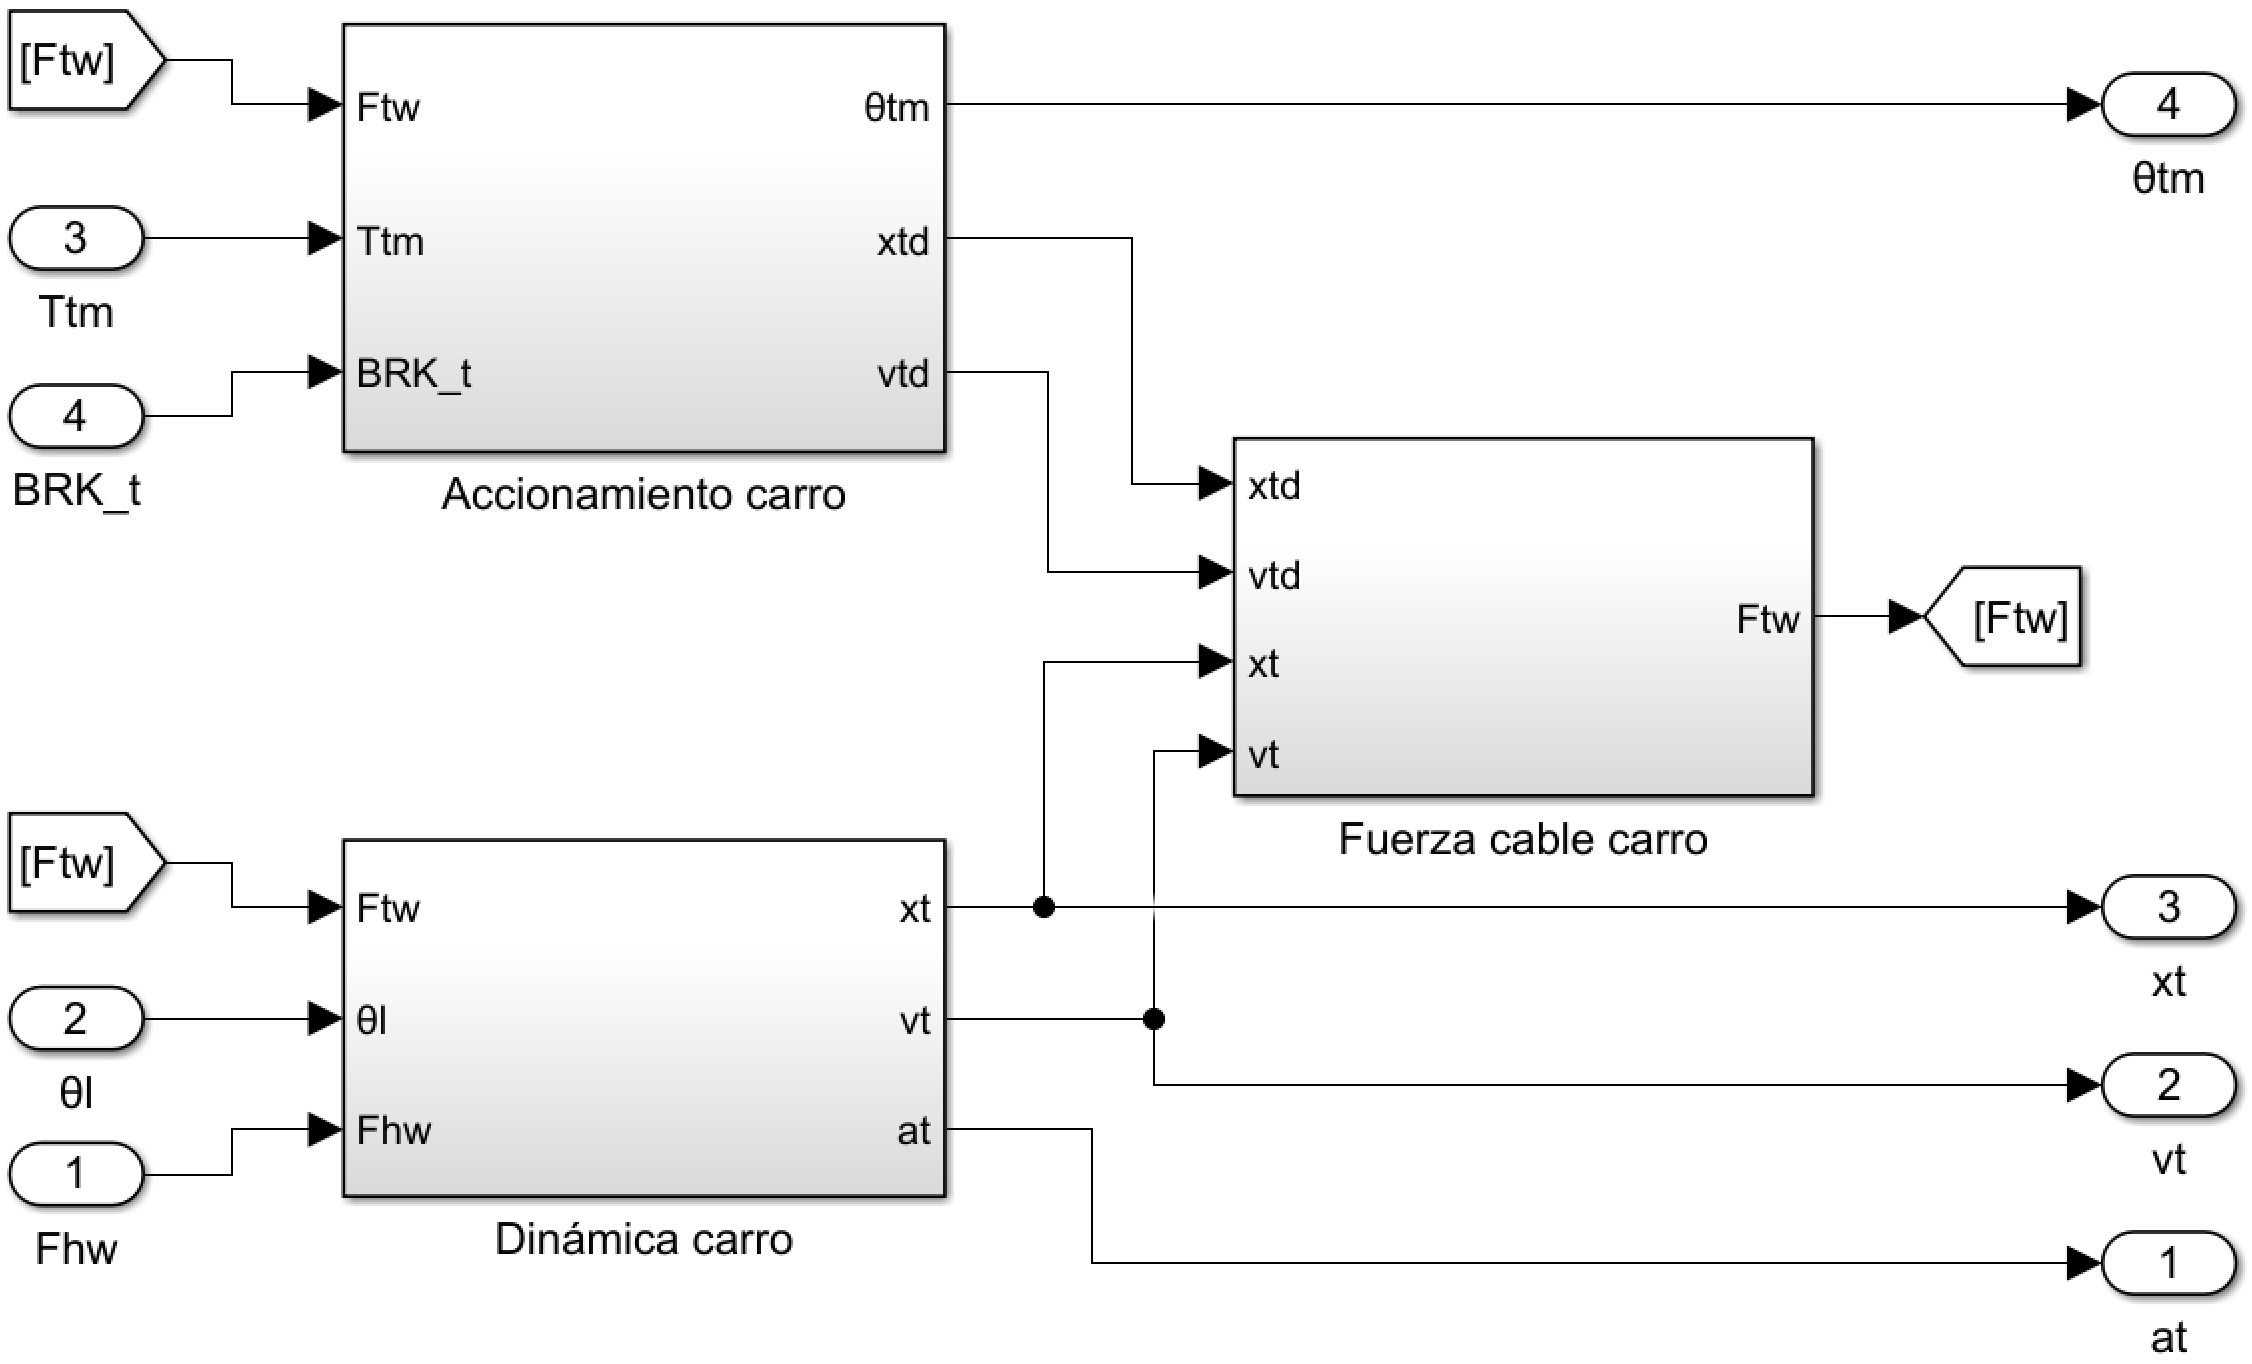
\includegraphics[width=1\textwidth]{carro_planta.png}
    \caption{Modelo del carro en Simulink (Trolley).}
\end{figure}

\subsection{Subsistema de Izaje (Hoist)}
El sistema de izaje controla la elevación de la carga mediante un mecanismo de tambor accionado por motor eléctrico, con un sistema de cableado (reeving) que introduce una relación de transmisión mecánica adicional.
\begin{figure}[H]
    \centering
    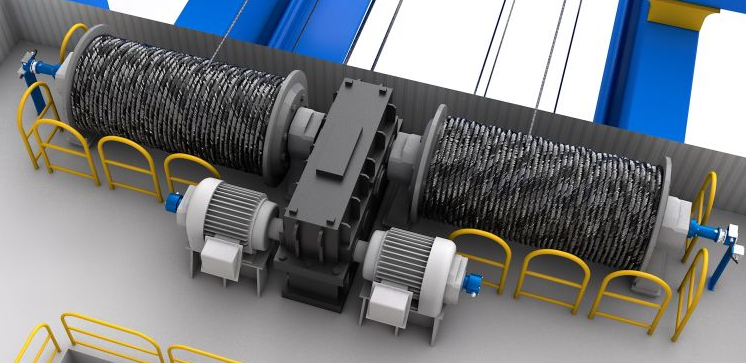
\includegraphics[width=1\textwidth]{hoist.png}
    \caption{Diagrama del subsistema de izaje (tambores-motores) (Hoist).}
    \label{fig:hoist}
\end{figure}

\subsubsection{Dinámica de la Carga Suspendida}
La carga se modela como una masa puntual concentrada en el centro de gravedad del conjunto Spreader/Contenedor, con 2 grados de libertad: traslación horizontal $x_l$ y vertical $y_l$. Su dinámica es híbrida, ya que sus parámetros (masa y geometría) cambian discretamente según el estado de los twistlocks y su interacción con el entorno cambia según si está suspendida o apoyada.

\subsubsection*{Definición de Masa y Geometría}
Los parámetros inerciales y geométricos dependen del estado discreto de los cerrojos (twistlocks), controlado por la señal lógica \textcolor{cyan}{$TLK$}. Según la especificación:
\begin{itemize}
    \item \textbf{Masa Total ($m_l$):}
    \begin{equation}
        m_l(\textcolor{cyan}{TLK}) = 
        \begin{cases} 
            M_s & \text{si } \textcolor{cyan}{TLK} = \text{Off (solo spreader)} \\
            M_s + M_{cX} & \text{si } \textcolor{cyan}{TLK} = \text{On (spreader + contenedor)}
        \end{cases}
    \end{equation}

    \item \textbf{Altura de la Carga ($h_c$):} Define la distancia desde el punto de suspensión hasta la base inferior (necesaria para calcular colisiones/apoyo).
    \begin{equation}
        h_c(\textcolor{cyan}{TLK}) = 
        \begin{cases} 
            0 & \text{si } \textcolor{cyan}{TLK} = \text{Off} \\
            H_c & \text{si } \textcolor{cyan}{TLK} = \text{On}
        \end{cases}
    \end{equation}
\end{itemize}

\subsubsection*{Ecuaciones de Movimiento}
Aplicando la segunda ley de Newton en el plano vertical, la aceleración de la carga resulta de la suma vectorial de: la tensión del cable, la gravedad y las fuerzas de reacción del entorno.
\begin{itemize}
    \item \textbf{Dinámica Horizontal (Ecuación de Balanceo):} La componente horizontal de la tensión del cable actúa como fuerza restauradora hacia la posición del carro.
    \begin{equation} \label{eq:carga_horiz}
        m_l(\textcolor{cyan}{TLK}) \, \frac{d \, v_{lx}(t)}{dt} = -2 F_{hw}(t) \, \sin\theta_l(t) + F_{cx}(t)
    \end{equation}
    \textit{Nota:} El signo negativo indica que si la carga está a la derecha ($\theta > 0$), la fuerza tira hacia la izquierda.

    \item \textbf{Dinámica Vertical (Ecuación de Izaje):}
    \begin{equation} \label{eq:carga_vert}
        m_l(\textcolor{cyan}{TLK}) \, \frac{d \, v_{ly}(t)}{dt} = 2 F_{hw}(t) \, \cos\theta_l(t) - m_l(\textcolor{cyan}{TLK}) \, g + F_{cy}(t)
    \end{equation}
\end{itemize}

\subsubsection*{Interacción con el Entorno (Modelo de Contacto)}
La carga interactúa con un perfil de obstáculos $y_{c0}(x,t)$ (suelo, barco, otros contenedores). Se define la penetración vertical $\delta_y$ como:
\[ \delta_y(t) = y_{c0}(x_l,t) - (y_l(t) - h_c(\textcolor{cyan}{TLK})) \]

Las fuerzas de reacción actúan solo cuando hay contacto ($\delta_y \ge 0$):
\begin{itemize}
    \item \textbf{Fuerza Vertical de Soporte ($F_{cy}$):} Modelo elástico-amortiguado (resorte $K_{cy}$ y amortiguador $b_{cy}$) que resiste la compresión.
    \begin{equation}
        F_{cy}(t) = 
        \begin{cases} 
            K_{cy} \, \delta_y(t) - b_{cy} \, v_{ly}(t) & \text{si } \delta_y(t) \ge 0 \text{ (Apoyado)} \\
            0 & \text{si } \delta_y(t) < 0 \text{ (Suspendido)}
        \end{cases}
    \end{equation}

    \item \textbf{Fuerza Horizontal de Fricción ($F_{cx}$):} Resistencia al arrastre horizontal, existente solo si hay contacto vertical.
    \begin{equation}
        F_{cx}(t) = 
        \begin{cases} 
            -b_{cx} \, v_{lx}(t) & \text{si } \delta_y(t) \ge 0 \\
            0 & \text{si } \delta_y(t) < 0
        \end{cases}
    \end{equation}
\end{itemize}

\subsubsection{Acoplamiento Elástico del Cable}
El cable de izaje se modela como un resorte-amortiguador. A diferencia del carro, su longitud desenrollada $l_h(t)$ cambia drásticamente, lo que afecta su rigidez y amortiguamiento.

Tanto la rigidez unitaria $k_{hwu}$ como el amortiguamiento unitario $b_{hwu}$ escalan con la longitud total del cable bajo tensión ($2 l_h(t) + L_{h0}$):
\begin{equation}
    K_{hw}(l_h) = \frac{k_{hwu}}{2 l_h(t) + L_{h0}} \quad ; \quad b_{hw}(l_h) = b_{hwu}\,(2 l_h(t) + L_{h0})
\end{equation}

La fuerza de tensión $F_{hw}$ se calcula solo si el cable está tenso ($l \ge l_h$):
\begin{equation} \label{eq:tension_izaje}
    F_{hw}(t) = 
    \begin{cases} 
        K_{hw}(l_h) \, \Delta L + b_{hw}(l_h) \, \Delta V & \text{si } l(t) \ge l_h(t) \text{ (Tenso)} \\
        0 & \text{si } l(t) < l_h(t) \text{ (Flojo/Slack)}
    \end{cases}
\end{equation}
Donde la elongación es $\Delta L = 2(l(t) - l_h(t))$ debido al reeving.

\subsubsection{Dinámica del Accionamiento}
El sistema posee dos frenos y una transmisión.
\begin{itemize}
    \item \textbf{Eje Lento (Tambor):} Posee el Freno de Emergencia ($T_{hEb}$).
    \begin{equation}
        J_{hd+hEb} \, \frac{d \, \omega_{hd}(t)}{dt} = T_{hd}(t) + T_{hEb}(\textcolor{cyan}{BRK_{hE}}) - b_{hd} \, \omega_{hd}(t) - T_{hdl}(t)
    \end{equation}
    \item \textbf{Eje Rápido (Motor):} Posee el Freno de Operación ($T_{hb}$).
    \begin{equation}
        J_{hm+hb} \, \frac{d \, \omega_{hm}(t)}{dt} = T_{hm}(t) + T_{hb}(\textcolor{cyan}{BRK_{h}}) - b_{hm} \, \omega_{hm}(t) - T_{hml}(t)
    \end{equation}
\end{itemize}

Relación cinemática del Reeving (2:1) y Tambor:
\begin{equation}
    v_h(t) = \frac{r_{hd} \, \omega_{hd}(t)}{2} = -\frac{d \, l_h(t)}{dt}
\end{equation}
El factor 2 divide la velocidad tangencial del tambor porque es un aparejo móvil.

\subsubsection*{Modelo de los Frenos Mecánicos de Operación y Emergencia}
A diferencia del carro, el sistema de izaje cuenta con dos sistemas de frenado independientes para garantizar la seguridad de la carga suspendida. Ambos operan bajo lógica "Normal Cerrado" (NC).
\begin{itemize}
    \item \textbf{Freno de Operación (Eje Rápido):} Ubicado en el eje del motor, actúa durante las paradas normales y el mantenimiento de posición (parking).
    \begin{equation} \label{eq:brake_hoist_op}
        T_{hb}(t,\textcolor{cyan}{BRK_{h}}) = 
        \begin{cases} 
            0 & \text{si } \textcolor{cyan}{BRK_h} = 1 \text{ (Energizado/Abierto)} \\
            -T_{hb\_Max} \, \tanh(b_{hb} \, \omega_{hm}(t)) & \text{si } \textcolor{cyan}{BRK_h} = 0 \text{ (Desenergizado/Cerrado)}
        \end{cases}
    \end{equation}
    \item \textbf{Freno de Emergencia (Eje Lento):} Ubicado directamente sobre el tambor, actúa solo ante fallas críticas (Nivel 0 de Protección) o parada de emergencia.
    \begin{equation} \label{eq:brake_hoist_emg}
        T_{hEb}(t,\textcolor{cyan}{BRK_{h}}) = 
        \begin{cases} 
            0 & \text{si } \textcolor{cyan}{BRK_{hE}} = 1 \text{ (Energizado/Abierto)} \\
            -T_{hEb\_Max} \, \tanh(b_{hEb} \, \omega_{hd}(t)) & \text{si } \textcolor{cyan}{BRK_{hE}} = 0 \text{ (Desenergizado/Cerrado)}
        \end{cases}
    \end{equation}
\end{itemize}

\subsubsection*{Modelo Equivalente Referido al Motor}
Dado que el Freno de Emergencia está en el eje lento, su torque también se divide por la relación de transmisión $i_h$ al reflejarlo.
\begin{equation}
    J_{eq,h} = J_{hm+hb} + \frac{J_{hd+hEb}}{i_h^2}  \quad ; \quad
    b_{eq,h} = b_{hm} + \frac{b_{hd}}{i_h^2}  \quad ; \quad
    T_{hEb,ref} = \frac{T_{hEb}}{i_h}
\end{equation}

\subsubsection{Modelo de Espacio de Estados para Simulación}
Finalmente, las ecuaciones diferenciales se ordenan despejando las derivadas de mayor orden para su implementación mediante bloques en Simulink.
\begin{itemize}
    \item \textbf{Accionamiento del izaje:}
    \begin{equation}\label{accionamiento_izaje}
        \frac{d\,\omega_{hm}(t)}{dt}
        = \frac{1}{J_{eq,h}}
        \left[
            T_{hm}(t)
            + T_{hb}(t,\textcolor{cyan}{BRK_h})
            + \frac{T_{hEb}(t,\textcolor{cyan}{BRK_{hE}})}{i_h}
            - b_{eq,h}\,\omega_{hm}(t)
            - \frac{r_{hd}}{i_h} \, F_{hw}(t)
        \right]
    \end{equation}
    donde $T_{hdl} = F_{hw}\,r_{hd}$ es el torque ejercido por el cable sobre el tambor.

    \item \textbf{Dinámica de la carga:}
    \begin{equation}\label{v_vertical}
        \frac{d\,v_{ly}(t)}{dt}
        = \frac{1}{m_l(\textcolor{cyan}{TLK})}
        \left[
            2\,F_{hw}(t)\cos\theta_l
            - m_l(\textcolor{cyan}{TLK})\,g
            + F_{cy}(t)
        \right]
    \end{equation}
    \begin{equation}\label{v_horizontal}
        \frac{d\,v_{lx}(t)}{dt}
        = \frac{1}{m_l(\textcolor{cyan}{TLK})}\left[-2 F_{hw}(t) \, \sin\theta_l(t) + F_{cx}(t)\right]
    \end{equation}

    \item \textbf{Posición de la carga:}
    \begin{equation}
        \frac{d\,y_l(t)}{dt} = v_{ly}(t)
    \end{equation}

    \item \textbf{Fuerza del cable de izaje:}
    \begin{equation}
        F_{hw}(t) =
        \begin{cases}
            2 K_{hw}(l_h) \, \left( l(t) - l_h(t) \right)
            + 2 b_{hw}(l_h) \, \left( \frac{d \, l(t)}{dt} - \frac{d \, l_h(t)}{dt} \right),
            & \text{si } l \ge l_h \text{ (Tenso)} \\[6pt]
            0, & \text{si } l < l_h \text{ (Flojo)}
        \end{cases}
    \end{equation}
    Nota: Se utiliza $\frac{dl}{dt}$ en lugar de $v_{ly}$ para considerar el estiramiento inducido por el balanceo ($\theta_l \neq 0$).

    \item \textbf{Longitud de cable desplegado:}
    \begin{equation}\label{l_desplegado}
        \frac{d\,l_h(t)}{dt}
        = -\,\frac{r_{hd}}{2\,i_h}\,\omega_{hm}(t)
    \end{equation}
    El signo negativo indica que una velocidad positiva del motor
    ($\omega_{hm} > 0$) enrolla el cable y reduce la longitud $l_h$.
\end{itemize}

\textbf{Variables auxiliares:}
\begin{itemize}
    \item Rigidez variable: $K_{hw}(l_h) = \frac{k_{hwu}}{2 l_h(t) + L_{h0}}$
    \item Amortiguamiento variable: $b_{hw}(l_h) = b_{hwu}\,(2 l_h(t) + L_{h0})$
    \item Longitud geométrica actual (Pitágoras): $l(t) = \sqrt{(x_l(t) - x_t(t))^2 + (Y_{t0} - y_l(t))^2} \quad$ ($Y_{t0}$ es la altura fija de poleas de izaje en el carro)
    \item Velocidad de cambio de longitud (para el amortiguamiento):
    \[ \frac{dl(t)}{dt} = \frac{(x_l(t) - x_t(t))(v_{lx}(t) - v_t(t)) - (Y_{t0} - y_l(t))v_{ly}(t)}{l(t)} \]
    \item Cálculo del ángulo de balanceo:
    \[ \theta_l = \text{atan2}\left(\frac{x_l(t) - x_t(t)}{Y_{t0} - y_l(t)}\right) \]
\end{itemize}

\begin{figure}[H]
    \centering
    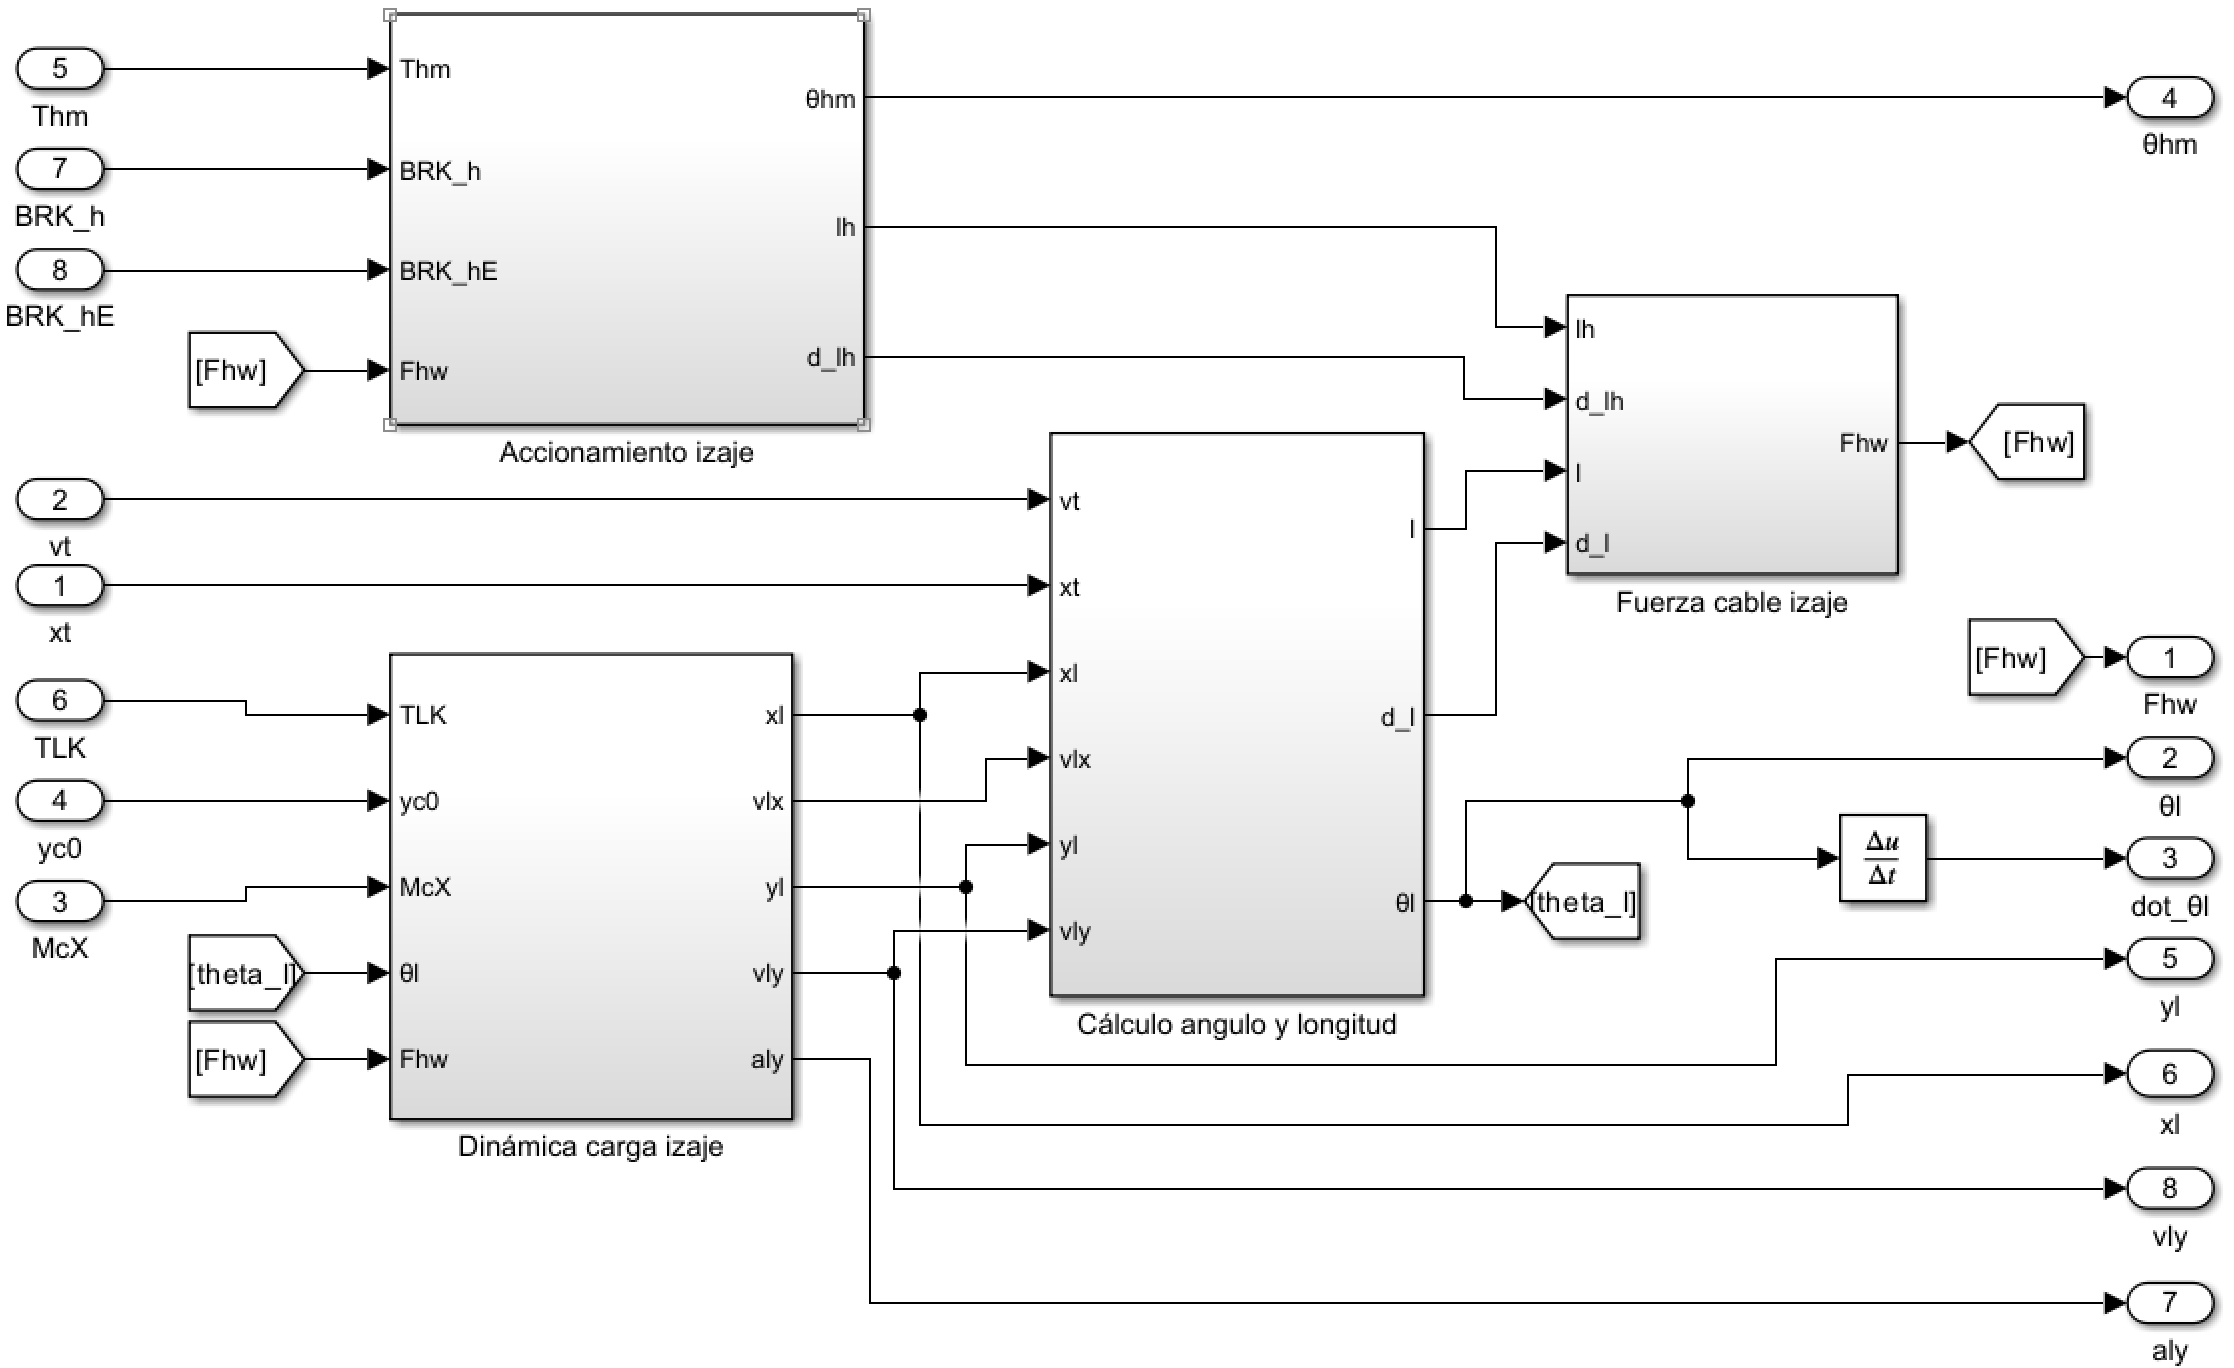
\includegraphics[width=1\textwidth]{izaje_planta.png}
    \caption{Modelo del izaje en Simulink (Hoist).}
\end{figure}

\subsection{Perfil 2D de Obstáculos}
El carro cuenta con un sistema de sensado LIDAR (escaner láser infrarojo 1D) para relevar el perfil topográfico de obstáculos $y_{c0}$ en el área de operación. Este perfil define la superficie efectiva con la que puede interactuar la carga suspendida (spreader + contenedor). El sensor está colocado en el carro, $3$m hacia adelante del spreader, y mide la distancia vertical instantánea desde el carro en movimiento hasta la pila de obstáculos.

Se puede discretizar la posicion del carro (y por lo tanto del spreader) en el rango $x_t \in [x_{t_{min}}, x_{t_{max}}]$ utilizando el ancho del contenedor $W_c$ como paso entre centros. Luego, la cantidad de posiciones discretas a lo largo de $x_t$:
\begin{equation}
    N_{x_t} = \text{floor}\left( \frac{x_{t_{max}} - x_{t_{min}}}{W_c} \right)+1
\end{equation}

Según la especificación se tiene que $x_{t_{min}}=-30\,$m (sobre el muelle) y $x_{t_{max}}=50\,$m (sobre el barco), y que $W_c=2.44\,$m (ancho de container estándar ISO), se obtiene que $N_{x_t} = 33$. Los posibles índices serán entonces:
\begin{equation}
    i = 1, 2, 3, \ldots, 33
\end{equation}
Luego, la última posición discreta corresponde a:
\begin{equation}
    x_{33} = -30\,\text{m} + (33-1) \cdot 2.44\,\text{m} = 48.08\,\text{m}
\end{equation}
Por lo que se verifica que el rango de discretización cubre todo el área de operación del carro sin exceder el límite de $x_{t_{max}}$.

Para simular el sensado del terreno, se crea un vector $h_{vec}$ de tamaño $N_{x_t}$ que es rellenado con valores de altura representativos del perfil de relieve del terreno real. De esa manera, a medida que el carro se desplaza, las mediciones tomadas por el sensor LIDAR se representan mediante la extracción de los valores de $h_{vec}$ y su guardado en un vector $y_{c0\_vec}$ también de tamaño $N_{x_t}$, e inicialmente nulo. Para saber si una posición ya ha sido escaneada, en memoria se almacena además un vector $is\_scanned\_vec$ también de tamaño $N_{x_t}$ con valores booleanos que indican si la posición correspondiente ya ha sido sensada o no. De esta manera, el sistema de control luego puede tomar diferentes decisiones según si el perfil de obstáculos por donde debe pasar el carro ya ha sido escaneado o no.

Se puede calcular el indice $i$ correspondiente a la posicion actual del sensor (teniendo en cuenta el offset respecto al carro) con:
\begin{equation}
    i = \text{floor}\left( \frac{(x_t(t)+3\,\text{m}) - x_{t_{min}}}{W_c} \right)
\end{equation}

El vector $y_{c0\_vec}$ se actualiza dinámicamente durante la operación de la grúa, permitiendo que el sistema de control y protección utilice el perfil de obstáculos más reciente para planificar movimientos seguros y evitar colisiones.

\subsection{Instrumentación y Sensores de Posición}
Para la retroalimentación del sistema de control y la protección automática, se modelan sensores de posición continua (encoders) y discretos (fines de carrera).

\subsubsection{Sistema de Encoders}
Conforme a la especificación, los sensores de posición son encoders absolutos o incrementales montados solidarios al eje de cada motor.
El sistema de control no recibe los ángulos directamente, sino que procesa estas señales para obtener las posiciones lineales equivalentes.
\begin{enumerate}
    \item \textbf{Encoder del Carro:} El sensor mide el ángulo acumulado del motor de carro, $\theta_{tm}(t)$. La señal de posición lineal se obtiene aplicando la relación de transmisión $i_t$ y el radio del tambor $r_{td}$:
    \begin{equation}
        x_{enc}(t) = \theta_{tm}(t) \, \frac{r_{td}}{i_t}
    \end{equation}

    \item \textbf{Encoder de Izaje:} El sensor mide el ángulo acumulado del motor de izaje, $\theta_{hm}(t)$. Se asume que el sistema se inicializa (homing) tal que $\theta_{hm}=0$ corresponde al nivel del muelle ($y=0$). Dado que un giro positivo del motor reduce la longitud del cable ($l_h$) y por ende aumenta la altura de la carga ($y$), la señal de retroalimentación $y_{enc}(t)$ se obtiene mediante:
    \begin{equation}
        y_{enc}(t) = \theta_{hm}(t) \, \left( \frac{r_{hd}}{2 \, i_h} \right)
    \end{equation}
    Esta señal representa la altura operativa de la carga.
\end{enumerate}

\subsubsection{Fines de Carrera}
La lógica de detección de límites se modela según la ubicación física descrita en las especificaciones, diferenciando entre sensores externos (viga) y sensores internos (tambor).
\begin{enumerate}
    \item \textbf{Fines de Carrera de Carro (Fijos en Viga):} Al estar montados físicamente sobre la estructura de la grúa, estos sensores detectan la posición real de la masa del carro $x_t(t)$, independientemente de la elongación del cable o la posición del motor.
    \begin{itemize}
        \item \textbf{Entrada:} Posición real del carro $x_t$.
        \item \textbf{Lógica de activación:}
        \begin{equation}
            FC_{t,\,\text{derecha}} = 
            \begin{cases} 
                0 & \text{si } x_t(t) < x_{t,max}  \\
                1 & \text{si } x_t(t) \ge x_{t,max} \quad (\text{Operativo}) \\
                1 & \text{si } x_t(t) \ge x_{t,max} + 0.5 \text{m} \quad (\text{Emergencia})
            \end{cases}
        \end{equation}
        (Análogamente para el retroceso (izquierda) hacia $x_{t,min}$).
    \end{itemize}
    \item \textbf{Fines de Carrera de Izaje (Rotativos en Tambor):} Al estar acoplados mecánicamente al eje del tambor, estos sensores detectan la cantidad de cable desenrollado. No miden la posición real de la carga (que varía con el balanceo).
    \begin{itemize}
        \item \textbf{Entrada:} Altura calculada por encoder $y_{enc}(t)$.
        \item \textbf{Lógica de activación:}
        \begin{equation}
            FC_{h,\,\text{superior}} = 
            \begin{cases}
                0 & \text{si } y_{enc}(t) < y_{h,max} \quad (\text{Operativo}) \\
                1 & \text{si } y_{enc}(t) \ge y_{h,max} \quad (\text{Operativo}) \\
                1 & \text{si } y_{enc}(t) \ge y_{h,max} + 0.5 \text{m} \quad (\text{Emergencia})
            \end{cases}
        \end{equation}
        (Análogamente para el descenso hacia $y_{h,min}$).
    \end{itemize}
\end{enumerate}

\subsection{Moduladores de Torque (Accionamientos)}
En la simulación de la planta física, no es posible aplicar la señal de control de referencia directamente como fuerza mecánica instantánea. Los accionamientos reales (variadores de frecuencia y motores eléctricos) presentan limitaciones tanto en su capacidad de torque máximo como en su velocidad de respuesta dinámica. Para modelar este comportamiento, se introducen bloques moduladores de torque para cada eje.

Estos moduladores cumplen tres funciones principales:
\begin{enumerate}
    \item \textbf{Lógica de frenos:} Anulan la entrega de torque del motor si los frenos mecánicos de retención se encuentran aplicados.
    \item \textbf{Saturación:} Limitan la magnitud del comando de torque para proteger el motor y respetar sus curvas de operación nominales.
    \item \textbf{Dinámica de primer orden:} Modelan el retardo electromagnético del motor mediante una constante de tiempo ($\tau$), que representa la inercia eléctrica del sistema.
\end{enumerate}

La dinámica general de los motores se representa mediante una ecuación diferencial de primer orden que vincula el torque limitado comandado ($T_{Lim}^*$) con el torque físico real entregado por el motor ($T(t)$):
$$\tau \cdot \frac{dT(t)}{dt} = T_{Lim}^*(t) - T(t)$$

Dado que la planta física es un sistema continuo, pero recibe señales de un controlador digital discreto, el valor comandado se mantiene constante mediante un retenedor de orden cero (ZOH) durante cada intervalo de muestreo.

\subsubsection{Modulador del Carro}
Para el sistema de traslación del carro, la saturación del motor posee un límite fijo ($T_{tm\_Max}$). Previo a la saturación, la señal de referencia digital ($T_{tm\_ref}$) se multiplica por el estado lógico del freno ($BRK_t$), obteniendo el comando efectivo $T_{tm}^*$. La ecuación de saturación por tramos de tiempo está dada por:

$$T_{tm\_Lim}^*(k \, T_{s2} \leq t < (k+1) \, T_{s2}) = \min(+T_{tm\_Max}, \max(-T_{tm\_Max}, T_{tm}^*(k \, T_{s2})))$$

$T_{s2}$ representa el tiempo de muestreo del controlador regulatorio (Nivel 2) a desarrollar, y $k$ es el índice del intervalo de muestreo actual. 

\subsubsection{Modulador de Izaje}
El mecanismo de izaje presenta una complejidad mayor debido a la redundancia de seguridad (freno de operación $BRK_h$ y freno de emergencia $BRK_{hE}$) y a la naturaleza de la curva de potencia del motor. 

El comando de torque efectivo requiere que ambos frenos estén liberados simultáneamente:
$$T_{hm}^* = T_{hm\_ref} \, BRK_h \, BRK_{hE}$$
A diferencia del carro, el límite de torque del motor de izaje no es constante. Para evitar exceder la potencia nominal del equipo a altas velocidades (zona de debilitamiento de campo o de potencia constante), el límite máximo permitido decae en función de la velocidad angular actual ($\omega_{hm}$), comparada con su velocidad nominal ($\omega_{hm\_rated}$). La restricción dinámica se modela como:
$$T_{hm\_Max\_dyn}(t) = T_{hm\_Max} \cdot \min \left( 1, \left( \frac{\omega_{hm\_rated}}{\omega_{hm}(t)} \right)^2 \right)$$
Finalmente, la saturación aplicada al accionamiento del izaje en cada instante de muestreo discreto resulta en:
$$T_{hm\_Lim}^*(k \, T_{s2} \leq t < (k+1) \, T_{s2}) = \min(+T_{hm\_Max\_dyn}(t), \max(-T_{hm\_Max\_dyn}(t), T_{hm}^*(k \, T_{s2})))$$

\subsection{Modelo de la Planta en Simulink}
\begin{figure}[H]
    \centering
    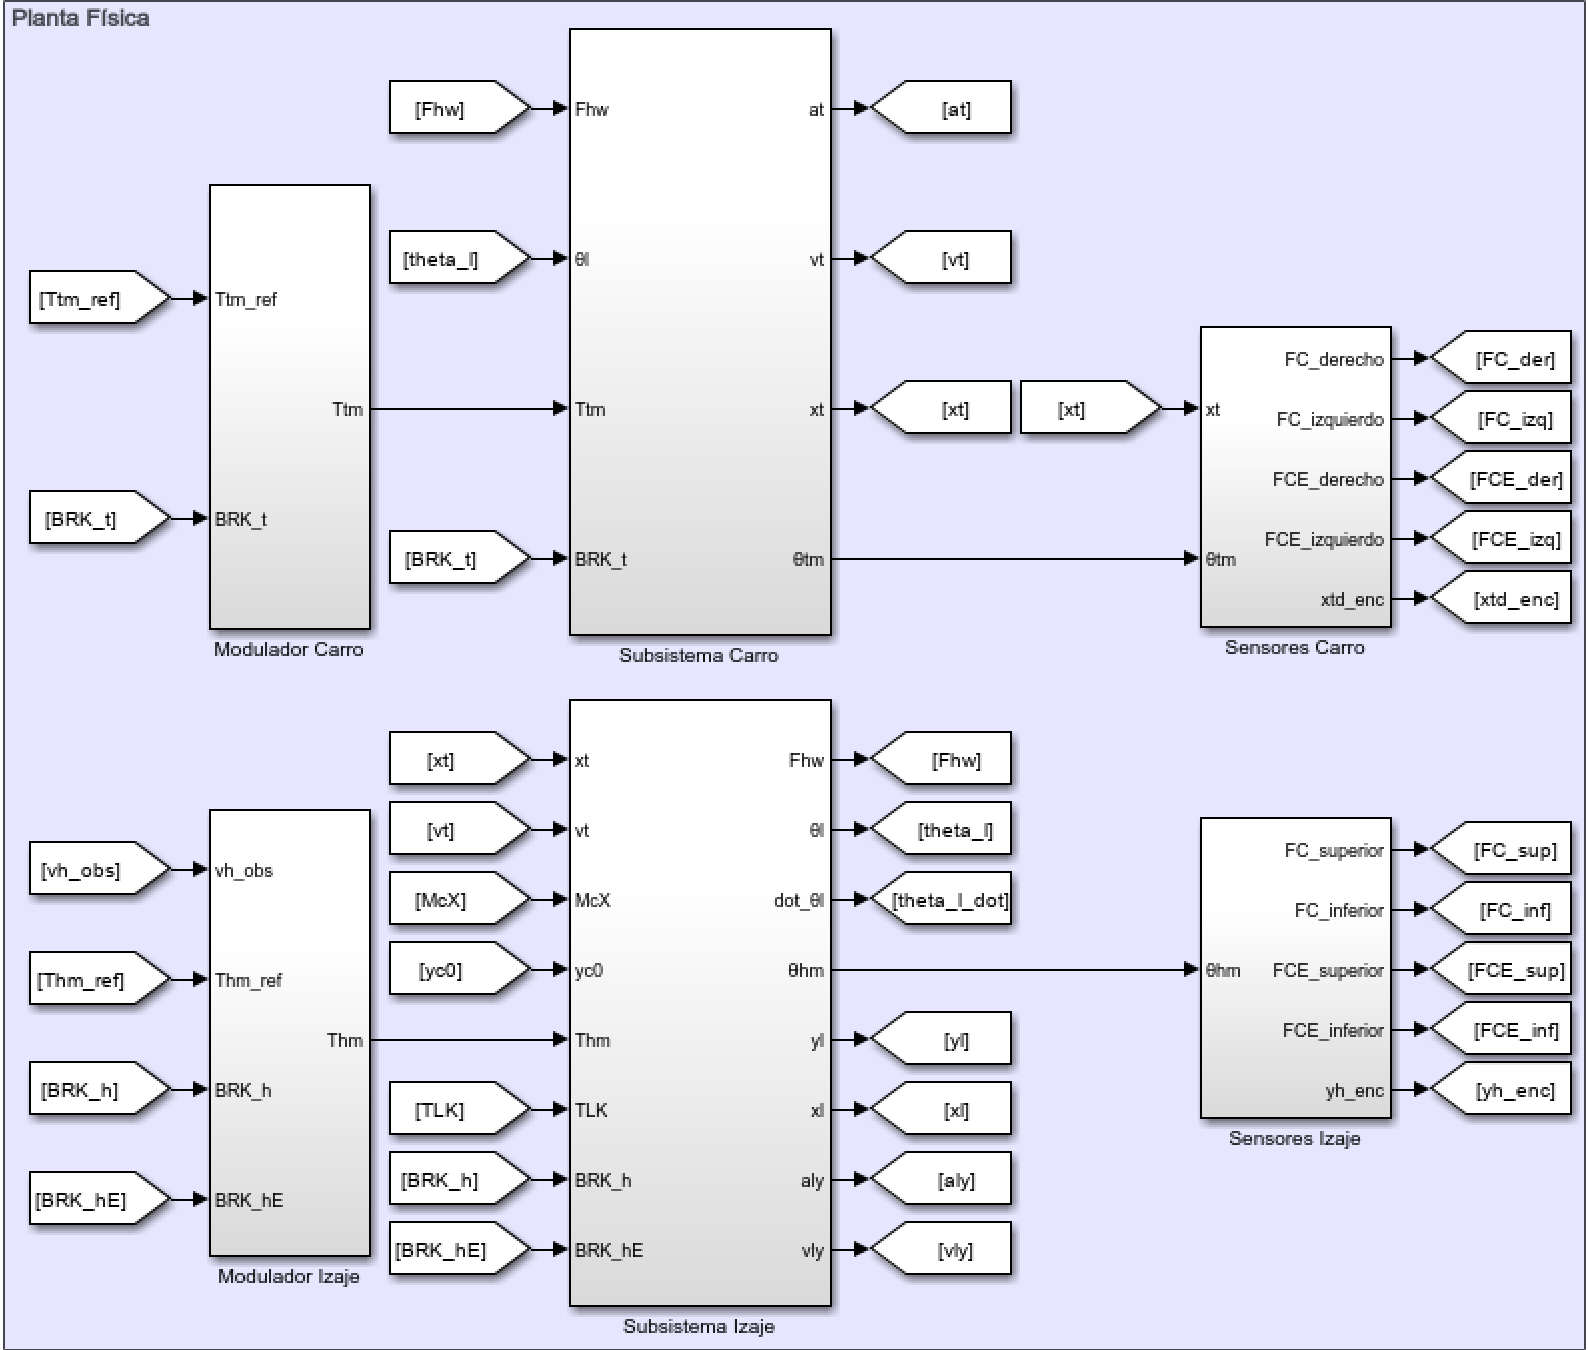
\includegraphics[width=1\textwidth]{planta_completa.png}
    \caption{Modelo de la Planta en Simulink.}
\end{figure}
Integrando todos los elementos descritos, se construye un modelo completo de la planta física en Simulink. Este modelo incluye bloques para cada subsistema, los moduladores de torque y los sensores de posición y fines de carrera. La interconexión de estos bloques permite simular la dinámica acoplada del sistema y evaluar el desempeño del controlador regulatorio a desarrollar a continuación.

\section{Diseño del Control Regulatorio (Nivel 2)}
El Nivel 2 corresponde al control regulatorio de las variables continuas del sistema. Su objetivo es garantizar que los accionamientos sigan referencias de posición, velocidad y aceleración con precisión y suavidad, respetando restricciones físicas (límites de recorrido, saturaciones de torque, corrientes máximas) y atenuando perturbaciones como el balanceo de la carga o variaciones de masa. Este nivel opera en tiempo discretizado mediante muestreo (Sampled CTDS) y se implementará con lazos de realimentación en cascada (corriente/torque, velocidad y posición), además de compensaciones para mejorar la respuesta transitoria.

En este proyecto, el control regulatorio se encarga de los subsistemas de traslación del carro y de izaje, coordinando sus dinámicas para lograr movimientos simultáneos y seguros. Las señales generadas en este nivel son consignas y comandos de accionamiento que luego son habilitados o bloqueados por el Control Supervisor (Nivel 1) y, ante eventos críticos, anulados por el Nivel de Protección (Nivel 0). De este modo, el Nivel 2 provee el desempeño continuo requerido, mientras los niveles superiores garantizan la lógica de operación y la seguridad global del sistema.

\subsection{Control de Izaje de la Carga}
Para el control de la carga en el izaje, se diseñó una arquitectura de Control Directo de Velocidad con Planificación Cinemática (Trayectoria $\to$ Velocidad $\to$ Torque). Esta estrategia evita los sobreesfuerzos mecánicos, disminuye el chattering y optimiza los tiempos de ciclo.

\subsubsection{Modelo de Izaje para Control de Velocidad}
Partiendo de la ecuación dinámica del izaje y considerando el sistema linealizado alrededor de un punto de operación, se asume que la dinámica del cable es rígida. 

La ecuación de balance de torques en el eje del motor es:
\begin{equation}
    J_{eq,h} \, \frac{d \, \omega_{hm}(t)}{dt} + b_{eq,h} \, \omega_{hm}(t) = T_{hm}(t) - T_{dist}(t)
\end{equation}
Donde $T_{dist}(t)$ es el torque perturbador que encapsula todas las dinámicas no lineales y externas al accionamiento:
\begin{equation}
    T_{dist}(t) = \underbrace{\frac{F_{hw}(t) \, r_{hd}}{i_h}}_{\text{Tensión de Cable}} + \underbrace{T_{hb}(t,\text{BRK}_h) + \frac{T_{hEb}(t,\text{BRK}_{hE})}{i_h}}_{\text{Fricción de Frenos}}
\end{equation}
Aplicando la Transformada de Laplace, la función de transferencia de la planta es:
\begin{equation} \label{eq:G_vel}
    G_{vel}(s) = \frac{\Omega_{hm}(s)}{T_{hm}(s)} = \frac{1}{J_{eq,h} \, s + b_{eq,h}}
\end{equation}
El polo mecánico del sistema es $P_{mec} = -b_{eq,h}/J_{eq,h}$. Dado que la fricción es muy baja en estos sistemas, el polo se encuentra muy cerca del origen ($P_{mec} \approx 0$), comportándose casi como un integrador puro.

\subsubsection{Diseño del Lazo Regulador (Control PI de Velocidad)}
Se utiliza un controlador Proporcional-Integral (PI) para asegurar error nulo de velocidad ante escalones de referencia y rechazo de perturbaciones de carga constantes.
\begin{equation}
    C_{vel}(s) = K_p + \frac{K_i}{s}
\end{equation}
La función de transferencia a lazo cerrado $T(s)$ resulta:
\begin{equation}
    T(s) = \frac{K_p \, s + K_i}{J_{eq,h} \, s^2 + (b_{eq,h} + K_p) \, s + K_i}
\end{equation}
Mediante el método de asignación de polos, se compara la ecuación característica con un polinomio de segundo orden deseado ($s^2 + 2\zeta\omega_ns + \omega_n^2$). Como $b_{eq,h}$ es muy pequeña en comparación con la inercia, las ecuaciones de diseño se simplifican:
\begin{equation} \label{eq:gains_hoist}
    K_p \approx 2 \, \zeta \, \omega_n \, J_{eq,h} \quad ; \quad K_i = \omega_n^2 \, J_{eq,h}
\end{equation}
Se selecciona $\omega_n \approx 8$ rad/s para asegurar rapidez sin excitar la resonancia del cable, y $\zeta \in [0.707, 1]$ para evitar sobrepasos. Esta sintonía garantiza la ``rigidez'' necesaria para sostener la carga.

El torque computado por el controlador PI en tiempo discreto es:
\begin{equation}
    T_{PID}(k) = K_p \, e_{vel}(k) + K_i \sum_{j=1}^{k} \frac{T_s}{2} \left[ e_{vel}(j) + e_{vel}(j-1) \right]
\end{equation}
donde $e_{vel}(k) = \omega_{ref}(k) - \omega_{hm}(k)$.

\subsubsection{Compensación de Gravedad (Feedforward)}
Para mejorar el desempeño, se añade un término de pre-alimentación ($T_{g,ff}$) a la salida del PID. Esto permite que el término integral ($K_i$) solo corrija errores de modelo, delegando el esfuerzo de sostener el peso estático al compensador.
\begin{equation}
        T_{g,ff} = \frac{m_l(\text{TLK}) \, g \, r_{hd}}{2 \, i_h}
\end{equation}
La ley de control del lazo regulador es: 
$T_{ref}(k) = T_{PID}(k) + T_{g,ff}$.

\subsubsection{Planificación Cinemática de Trayectorias}
En lugar de un lazo de posición tradicional que persigue una coordenada espacial, la referencia de velocidad $\omega_{ref}(k)$ es dictada por un algoritmo supervisor de trayectorias en el control Supervisor. Este planificador evalúa el estado del entorno (obstáculos, alturas de crucero) y genera una velocidad requerida ($v_{req}$) basada en una ley PD hacia un objetivo dinámico $y_{target}(k)$:
\begin{equation}
    v_{req}(k) = K_{p} \, \bigl(y_{target}(k) - y_{real}(k)\bigr) + K_{d} \, v_{y}(k)
\end{equation}
El valor de $y_{target}$ es gestionado por un autómata que garantiza la evasión de colisiones antes de habilitar el descenso. 

\subsubsection{Saturación Dinámica por Límite de Potencia}
Para respetar la curva de potencia constante del motor, el comando de velocidad generado por el planificador se limita dinámicamente en función de la carga izada estimada ($\hat{m}_l$). Se define una masa base $M_{base}$ a partir de la cual el accionamiento ya no puede sostener la velocidad mecánica máxima ($v_{h,max}$) sin exceder su potencia nominal ($P_{h,nom}$):
\begin{equation}
    v_{h,limit}(\hat{m}_l) = 
    \begin{cases} 
        v_{h,max} & \text{si } \hat{m}_l < M_{base} \\
        \frac{P_{h,nom}}{\hat{m}_l \, g} & \text{si } \hat{m}_l \ge M_{base}
    \end{cases}
\end{equation}

Finalmente, la señal saturada se convierte a velocidad angular, conformando la referencia maestra que ingresa al lazo regulador de velocidad:
\begin{equation}
    v_{ref}(k) = \text{sat}\left( v_{req}(k), \, \pm v_{h,limit}(\hat{m}_l) \right)
\end{equation}
\begin{equation}
    \omega_{ref}(k) = v_{ref}(k) \left( \frac{2 \, i_h}{r_{hd}} \right)
\end{equation}

\subsection{Control de Traslación del Carro}
Para el control del carro, se diseñó la misma arquitectura de Control Directo de Velocidad con Planificación Cinemática (Trayectoria $\to$ Velocidad $\to$ Torque).

\subsubsection{Modelo del Carro para Control de Velocidad}
Para el diseño del lazo interno de velocidad del carro, se adopta un modelo simplificado traslacional alrededor del punto de operación. Este modelo se obtiene a partir de la ecuación (\ref{eq:carro_newton}). En esta aproximación se desprecia la dinámica rotacional interna del accionamiento y se agrupan los acoplamientos mecánicos y perturbaciones externas en una fuerza perturbadora equivalente. Así, la dinámica horizontal del carro puede escribirse como:
\begin{equation}
    M_t\,\frac{d \, v_t(t)}{dt} + b_t\,v_t(t) = F_{cmd}(t) - F_{dist}(t)
\end{equation}
donde
\begin{equation}
    F_{cmd}(t)=K_f\,T_{tm}(t)
\end{equation}
y
\begin{equation}
    F_{dist}(t) = \underbrace{F_{tw}(t)}_{\text{Fuerza del cable}}
    - \underbrace{F_{coupling}(t)}_{\text{Acoplamiento con la carga}}
    + \Delta_{model}(t)
\end{equation}
siendo $T_{tm}(t)$ el torque aplicado por el motor y $K_f$ la ganancia equivalente fuerza--torque del conjunto variador--motor--transmisión. En este caso:
\begin{equation}
    K_f = \frac{i_t}{r_{td}}
\end{equation}
ya que el torque en el tambor cumple $T_{td}=i_t\,T_{tm}$ y la fuerza lineal equivalente sobre el carro resulta $F_{cmd}=T_{td}/r_{td}$.

Aplicando la Transformada de Laplace, la función de transferencia simplificada de la planta velocidad--mando queda:
\begin{equation}
    G_{vel,t}(s) = \frac{V_t(s)}{T_{tm}(s)} = \frac{K_f}{M_t\,s + b_t}
\end{equation}
El polo mecánico resulta $P_{mec} = -b_t/M_t$. Dado que el rozamiento equivalente es pequeño frente a la inercia dominante del carro, para la sintonía se adopta la aproximación:
\begin{equation}
    G_{vel,t}(s) \approx \frac{K_f}{M_t\,s}
\end{equation}

\subsubsection{Diseño del Lazo Regulador (Control PI de Velocidad)}
Se utiliza un controlador PI para asegurar error nulo de velocidad ante escalones de referencia y buen rechazo de perturbaciones constantes:
\begin{equation}
    C_{vel}(s) = K_p + \frac{K_i}{s}
\end{equation}
La función de transferencia a lazo cerrado $T(s)$ resulta:
\begin{equation}
    T(s) = \frac{C_{vel}(s) \, G_{vel,t}(s)}{1 + C_{vel}(s) \, G_{vel,t}(s)}
\end{equation}
Sustituyendo $C_{vel}(s)$ y $G_{vel,t}(s) \approx \frac{K_f}{M_t\,s}$:
\begin{equation}
    T(s) =
    \frac{\left(K_p + \frac{K_i}{s}\right)\frac{K_f}{M_t\,s}}
    {1 + \left(K_p + \frac{K_i}{s}\right)\frac{K_f}{M_t\,s}}
\end{equation}
Operando algebraicamente, se obtiene:
\begin{equation}
    T(s) = \frac{K_p K_f\,s + K_i K_f}{M_t\,s^2 + K_p K_f\,s + K_i K_f}
\end{equation}
por lo que la ecuación característica de segundo orden queda:
\begin{equation}
    M_t\,s^2 + K_p K_f\,s + K_i K_f
\end{equation}
Se iguala con un polinomio deseado de segundo orden:
\begin{equation}
    s^2 + 2\,\zeta\,\omega_n\,s + \omega_n^2
\end{equation}
obteniéndose las ganancias:
\begin{equation}
    K_p = \frac{2\,\zeta\,\omega_n\,M_t}{K_f}, \quad
    K_i = \frac{\omega_n^2\,M_t}{K_f}
\end{equation}
La selección de $\omega_n$ se realiza en función del ancho de banda deseado del carro y las limitaciones de aceleración; típicamente se toma $\zeta \in [0.7,1]$ para evitar sobrepasos.

El torque de referencia en tiempo discreto es:
\begin{equation}
    T_{tm}^\ast(k) = K_p\,e_v(k) + K_i \sum_{j=1}^{k} \frac{T_s}{2}\left[e_v(j) + e_v(j-1)\right]
\end{equation}
con $e_v(k) = v_t^\ast(k) - v_t(k)$ y $T_s$ el período de muestreo.

\subsubsection{Planificación Cinemática de Trayectorias}
Al igual que en el izaje, en lugar de un lazo de posición tradicional que persigue una coordenada espacial, la referencia de velocidad es dictada por un algoritmo supervisor de trayectorias en el control Supervisor. Se genera una velocidad requerida ($v_{req}$) basada en una ley PD hacia un objetivo dinámico $x_{target}(k)$:
\begin{equation}
    v_{req}(k) = K_{p} \, \bigl(x_{target}(k) - x_{real}(k)\bigr) + K_{d} \, v_{x}(k)
\end{equation}
El valor de $x_{target}$ es gestionado por un autómata que garantiza la evasión de colisiones antes de generar movimiento horizontal. 

\subsection{Diseño del Controlador de Balanceo (Anti-Sway)}
Para la implementación del sistema de control de oscilación de la carga, se ha optado por una estrategia de Control Desacoplado, en lugar de un control basado en el modelo dinámico completo del sistema. A continuación, se fundamenta esta decisión y se deduce la ley de control utilizada.

\subsubsection{Estructura Desacoplada}
El sistema de la grúa planteado posee dos dinámicas con escalas de tiempo claramente separadas:
\begin{enumerate}
    \item \textbf{Dinámica del Accionamiento (Lazo de Velocidad):} El control de velocidad del motor del carro tiene una respuesta rápida (tiempo de establecimiento $< 100$ ms).
    \item \textbf{Dinámica del Péndulo:} La oscilación de la carga es un fenómeno lento, con periodos naturales en el orden de los 2 a 12 segundos (dependiendo de la altura de izaje $l_h$).
\end{enumerate}

Bajo la hipótesis de que el lazo de velocidad está correctamente sintonizado, se asume que la velocidad real del carro $v_t$ sigue a la referencia de velocidad $v_{ref}$ con una dinámica despreciable:
\begin{equation}
    v_t(t) \approx v_{ref}(t)
\end{equation}
Esta asunción permite desacoplar la dinámica del actuador (masa del carro y fricción) de la dinámica pendular, simplificando significativamente el diseño del controlador externo.

\subsubsection{Deducción de la Ley de Control No Lineal}
A partir del modelo dinámico (Ley de Newton) de un péndulo simple excitado por la aceleración del carro $\ddot{x}_t$, la ecuación de movimiento está dada por:
\begin{equation}
    \ddot{\theta}_l = -\frac{g}{l_h}\sin(\theta_l) - \frac{\ddot{x}_t}{l_h}\cos(\theta_l)
    \label{eq:pendulo_nolineal}
\end{equation}
En esta arquitectura, la referencia de velocidad total enviada al variador del carro se compone de la velocidad de trayectoria planificada más la acción de control antibalanceo: $v_{ref} = v_{traj} + v_{sway}$. 
Se define entonces una ley de control antibalanceo proporcional al ángulo de oscilación:
\begin{equation}
    v_{sway} = K_{sway} \, \theta_l
    \label{eq:ley_control}
\end{equation}
La aceleración resultante del carro impuesta sobre el pivote del péndulo será la derivada de la referencia total:
\begin{equation}
    \ddot{x}_t \approx \dot{v}_{ref} \approx \dot{v}_{traj} + \frac{d}{dt}(K_{sway} \, \theta_l) = \dot{v}_{traj} + K_{sway} \, \dot{\theta}_l
\end{equation}
Sustituyendo esta expresión en la ecuación no lineal (\ref{eq:pendulo_nolineal}) y agrupando los términos dependientes del estado del péndulo a la izquierda, se obtiene la ecuación diferencial del sistema en lazo cerrado:
\begin{equation}
    \ddot{\theta}_l + \left( \frac{K_{sway}}{l_h} \cos(\theta_l) \right) \dot{\theta}_l + \frac{g}{l_h}\sin(\theta_l) = -\frac{\dot{v}_{traj}}{l_h}\cos(\theta_l)
    \label{eq:lazo_cerrado_nolineal}
\end{equation}
Este resultado desmuestra que la cinemática del sistema transforma la señal de velocidad inyectada en un término de amortiguamiento viscoso no lineal. Dado que en la operación normal de la grúa el ángulo de oscilación está acotado ($-\pi/2 < \theta_l < \pi/2$), el término $\cos(\theta_l)$ es estrictamente positivo. Esto garantiza que el coeficiente de amortiguamiento sea siempre mayor a cero, asegurando la extracción continua de energía cinética del péndulo y la estabilidad del sistema ante cualquier ángulo operativo, sin depender de aproximaciones de ángulos pequeños. La aceleración de la trayectoria $\dot{v}_{traj}$ actúa únicamente como una fuerza forzante acotada.

\subsubsection{Sintonía por Linealización Local (Gain Scheduling)}
Si bien la estabilidad está garantizada, para determinar analíticamente el valor óptimo de la ganancia $K_{sway}$ se evalúa el comportamiento del sistema en las cercanías del punto de equilibrio estable ($\theta_l = 0$, $\dot{\theta}_l = 0$). El error es casi despreciable para ángulos de entre $10^\circ$ y $5^\circ$, y esto permite no solo mayor eficiencia computacional sino también evitar singularidades.

Evaluando la ecuación (\ref{eq:lazo_cerrado_nolineal}) alrededor del origen ($\cos(\theta_l) \to 1$ y $\sin(\theta_l) \to \theta_l$), la dinámica local se reduce a:
\begin{equation}
    \ddot{\theta}_l + \left( \frac{K_{sway}}{l_h} \right) \dot{\theta}_l + \left( \frac{g}{l_h} \right) \theta_l = 0
\end{equation}
Para garantizar un desempeño uniforme frente a la variación de la longitud del cable, se comparan los coeficientes de esta ecuación con la ecuación canónica de un sistema de segundo orden ($s^2 + 2\,\zeta\,\omega_n \,s + \omega_n^2 = 0$), donde la frecuencia natural es $\omega_n = \sqrt{g/l_h}$. Igualando el término de amortiguamiento:
\begin{equation}
    \frac{K_{sway}}{l_h} = 2 \, \zeta \, \omega_n \implies K_{sway} = 2 \, \zeta \, l_h \, \sqrt{\frac{g}{l_h}}
\end{equation}
Simplificando, obtenemos la ganancia para un amortiguamiento crítico ($\zeta = 1$):
\begin{equation}
    K_{sway}(l_h) = 2 \,\sqrt{g \, l_h}
\end{equation}
Dado que la altura de izaje determina directamente la dinámica del péndulo, se implementa una estrategia de \textit{gain scheduling}, ajustando la ganancia $K_{sway}$ dinámicamente en función de $l_h$ para mantener las raíces del polinomio característico local invariantes durante toda la operación.

Esta ganancia teórica produce un amortiguamiento perfecto de la oscilación. Sin embargo, en la práctica esto genera correcciones horizontales notorias. Para evitar sobrecorrecciones en la posición objetivo de la carga, se debe subamortiguar el balanceo. Después de varias pruebas, se seleccionó $\zeta = 0.45$ para lograr un compromiso entre amortiguamiento efectivo y estabilidad robusta. Esto genera oscilaciones adicionales pequeñas, pero a cambio la posición de la carga se mantiene más cercana a la deseada, sin introducir retrasos excesivos.

\subsection{Observadores de Estado}
Se puede notar de las ecuaciones desarrolladas que la realimentación de velocidad es un parámetro crítico para garantizar la estabilidad de los lazos de velocidad. Dado que la planta física cuenta únicamente con mediciones de posición a través de encoders, la obtención de la velocidad mediante una derivada directa amplifica drásticamente el ruido de cuantificación de los sensores, desestabilizando la señal de control.

Para solucionar este problema y obtener una estimación limpia de la velocidad ($\hat{\omega}$), se implementan observadores de estado extendidos. Estos bloques combinan un modelo físico-matemático del sistema con un lazo de corrección basado en el error de estimación de posición.

El error de estimación se define como la diferencia entre la posición angular medida por el encoder y la posición estimada internamente por el observador:
$$e_{\theta} = \theta_{enc} - \hat{\theta}$$
Este error alimenta tres ganancias de corrección ($L_1$, $L_2$ y $L_3$) que ajustan la dinámica del modelo para forzar la convergencia de los estados estimados hacia los estados reales de la planta. Las ecuaciones diferenciales que rigen la actualización de los estados en el observador están dadas por:
$$\dot{\hat{\theta}} = \hat{\omega} + L_1 \, e_{\theta}$$
$$\dot{\hat{\omega}} = \frac{1}{J_{eq}} \left( T_{ref} - b_{eq} \, \hat{\omega} + L_3 \int e_{\theta} \, dt \right) + L_2 \, e_{\theta}$$
Donde:
\begin{itemize}
    \item $J_{eq}$ y $b_{eq}$ representan la inercia y fricción viscosa equivalentes reflejadas al eje del motor.
    \item $T_{ref}$ es el torque de referencia comandado por el lazo de velocidad interno.
    \item $L_3 \int e_{\theta} \, dt$ actúa como un estimador de perturbaciones, acumulando el error para compensar dinámicas no modeladas o variaciones de carga.
\end{itemize}

La arquitectura del observador es idéntica tanto para el mecanismo del carro como para el de izaje. Sin embargo, en el eje de izaje se introduce un término adicional de pre-compensación $T_{grav} = M_s \, g \, \frac{r_{hd}}{2 \, i_h}$ para contrarrestar el peso en vacío del spreader ($M_s$), evitando así un error de estimación transitorio en el instante de arranque.

Finalmente, la velocidad lineal observada ($\hat{v}$) que retroalimenta al controlador regulatorio principal se obtiene mediante la relación de transmisión cinemática de cada mecanismo respectivo:
$$\hat{v} = \hat{\omega} \cdot k_{out}$$
Siendo la constante de conversión $k_{out} = \frac{r_{td}}{i_t}$ para el sistema del carro y $k_{out} = \frac{r_{hd}}{2 i_h}$ para el sistema de izaje.

\subsubsection{Cálculo de Ganancias}
Para determinar los valores empíricos de las ganancias de corrección vectoriales $L = [L_1, L_2, L_3]^T$, se empleó la técnica de asignación de polos (Pole Placement) sobre un modelo de la planta en el espacio de estados aumentado.

El sistema mecánico del accionamiento se modeló definiendo como variables de estado la posición $x_1 = \theta$, la velocidad $x_2 = \omega$ y un estado extendido $x_3 = T_{dist}$, el cual representa el torque de perturbación total no modelado (acción integral). El sistema continuo aumentado resulta:
$$\dot{x} = A_{aug} \, x + B_{aug} \, u$$
$$y = C_{aug} \, x$$
Donde las matrices dinámicas del sistema son:
$$A_{aug} = \begin{bmatrix} 0 & 1 & 0 \\ 0 & -\frac{b_{eq}}{J_{eq}} & \frac{1}{J_{eq}} \\ 0 & 0 & 0 \end{bmatrix}, \quad C_{aug} = \begin{bmatrix} 1 & 0 & 0 \end{bmatrix}$$

La sintonía de este observador se rige por el principio de separación de anchos de banda. Para garantizar que la dinámica de estimación sea lo suficientemente veloz y no introduzca retardos de fase en el lazo de control regulatorio, la dinámica del observador se diseñó para ser significativamente más rápida que la dinámica de la planta. Específicamente, el polo base del observador ($\omega_{obs}$) se ubicó de manera que su respuesta sea $20$ veces más rápida que el polo dominante de la planta a lazo abierto ($p_{planta} = -b_{eq}/J_{eq}$).

Finalmente, mediante la función \textit{place}, se calculó el vector de ganancias $L$ que fuerza a la matriz característica del error del observador a poseer los autovalores deseados. 

Cabe destacar una consideración numérica importante en la implementación computacional: la función \textit{place} presenta inestabilidades e inconvenientes para invertir matrices cuando se exige la asignación de autovalores repetidos exactos. Para evitar este comportamiento numérico sin alterar la dinámica real del estimador, los tres polos del observador se separaron levemente entre sí (con variaciones del $1\%$ al $2\%$ respecto a la frecuencia base $\omega_{obs}$). Esta técnica asegura un cálculo robusto de las ganancias y garantiza una convergencia asintótica de las estimaciones $\hat{\theta}$, $\hat{\omega}$ y del torque de perturbación $\hat{T}_{dist}$.

\subsection{Modelo del Controlador Regulatorio en Simulink}
\begin{figure}[H]
    \centering
    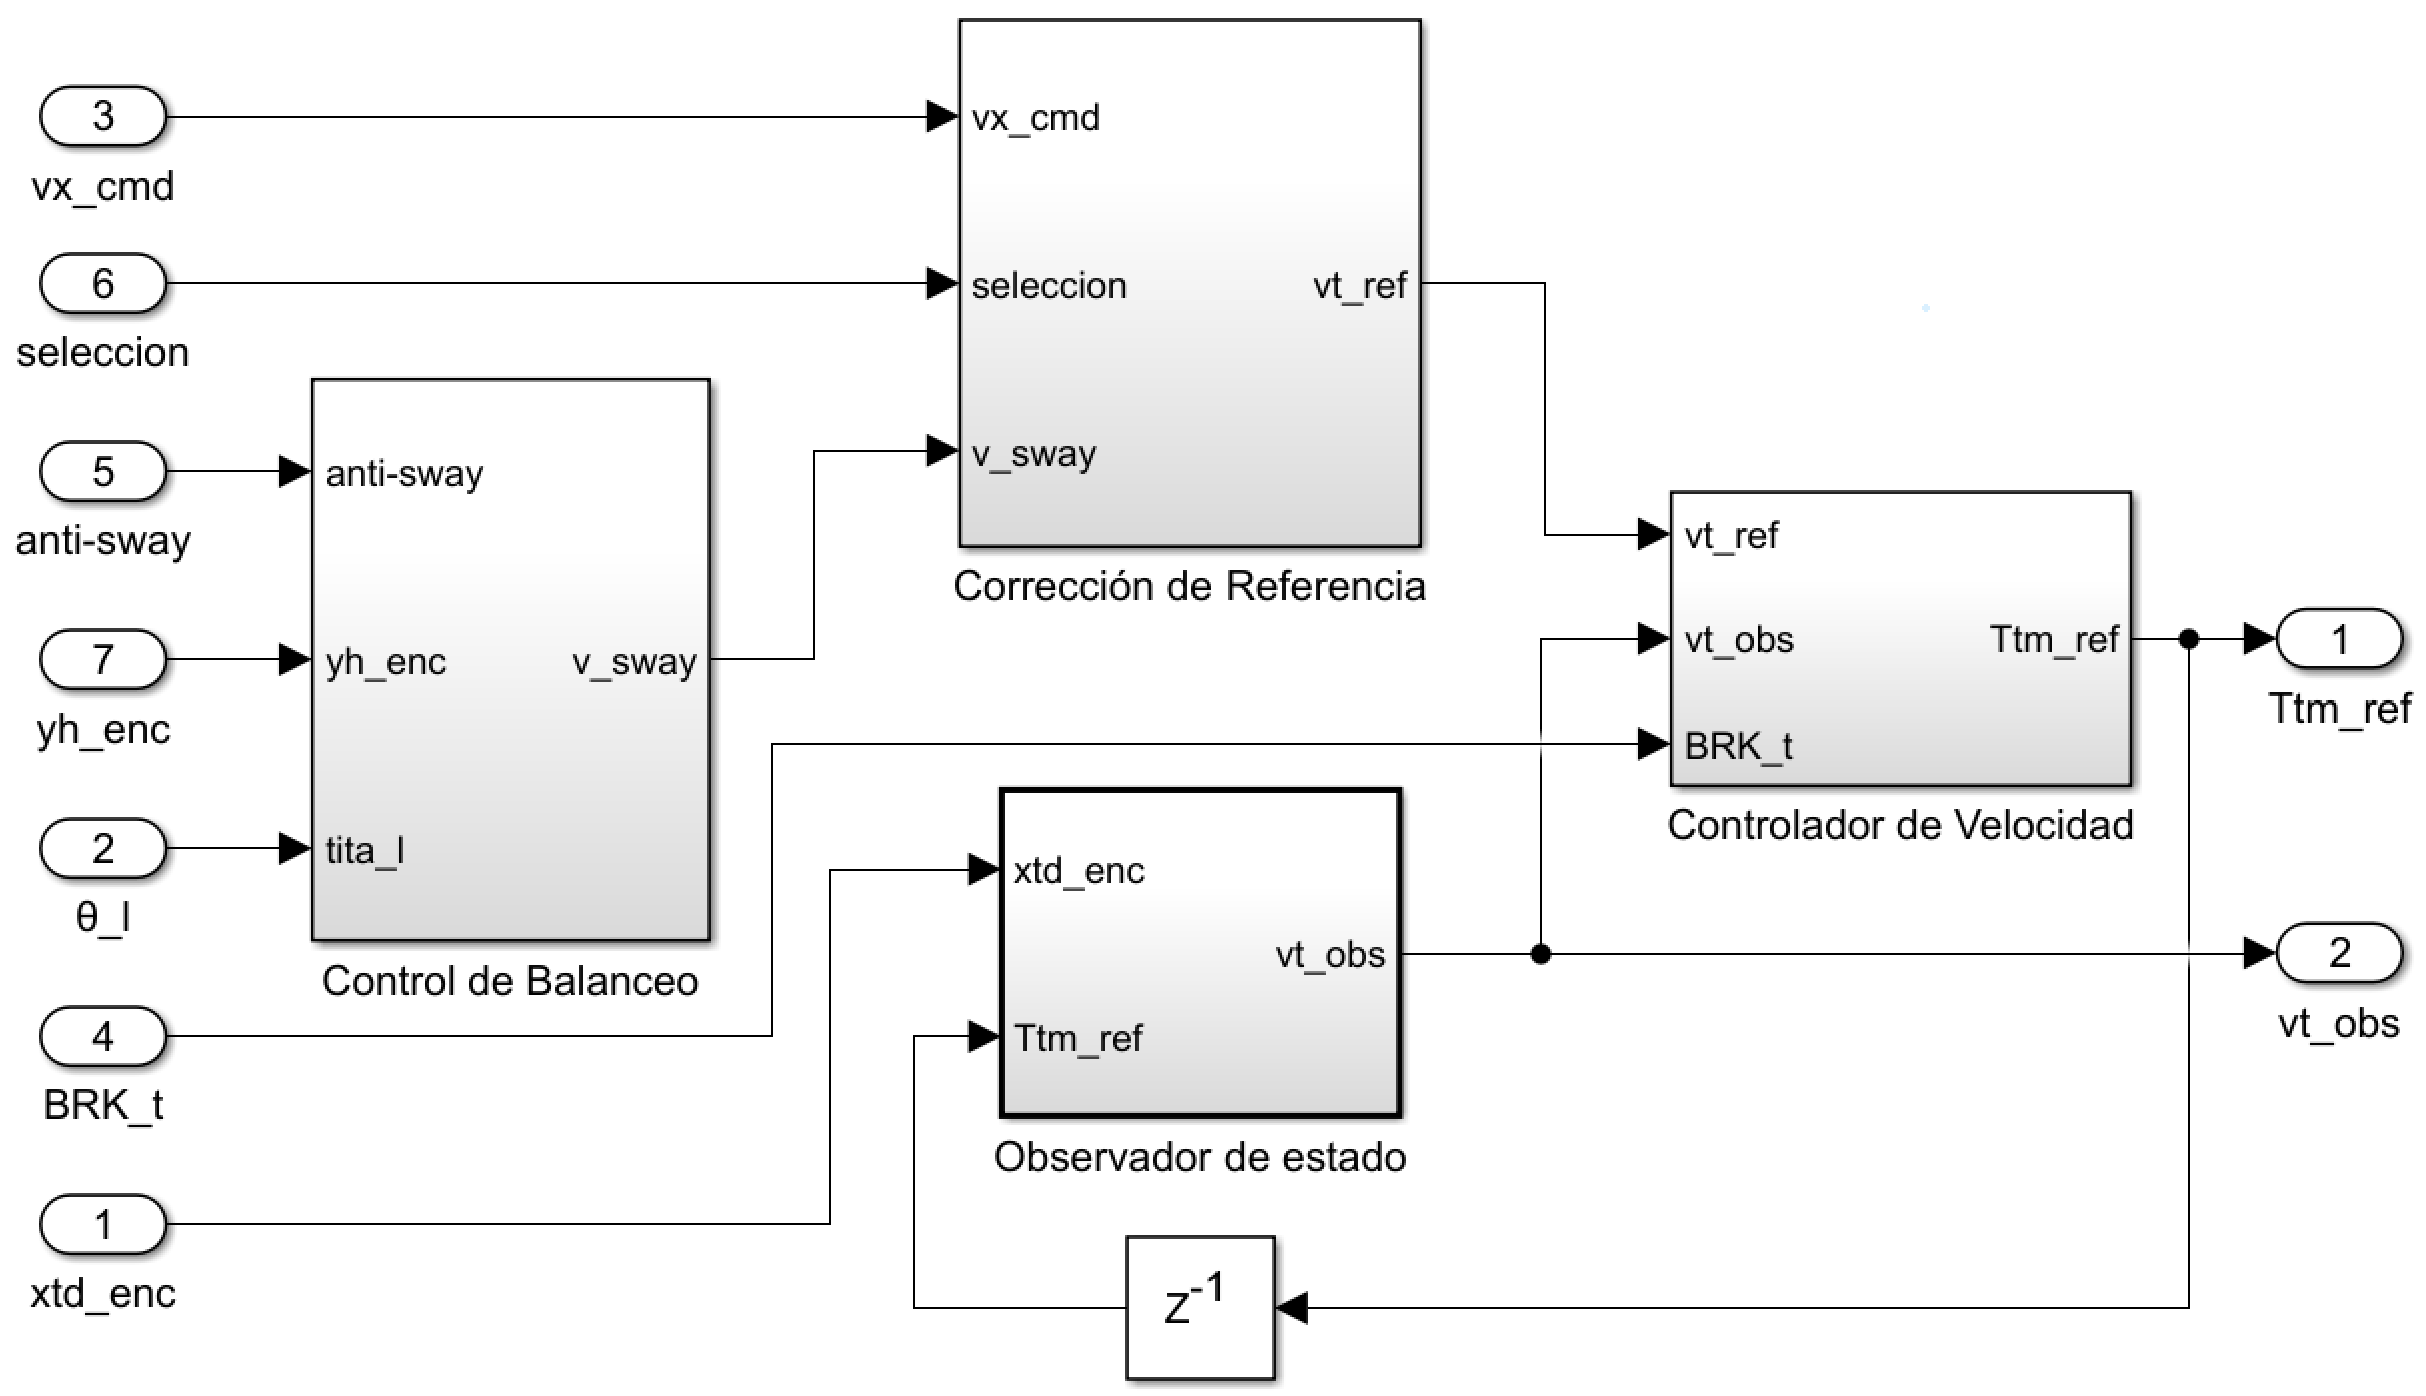
\includegraphics[width=1\textwidth]{control_carro2.png}
    \caption{Control Regulatorio del Carro (Trolley).}
\end{figure}
\begin{figure}[H]
    \centering
    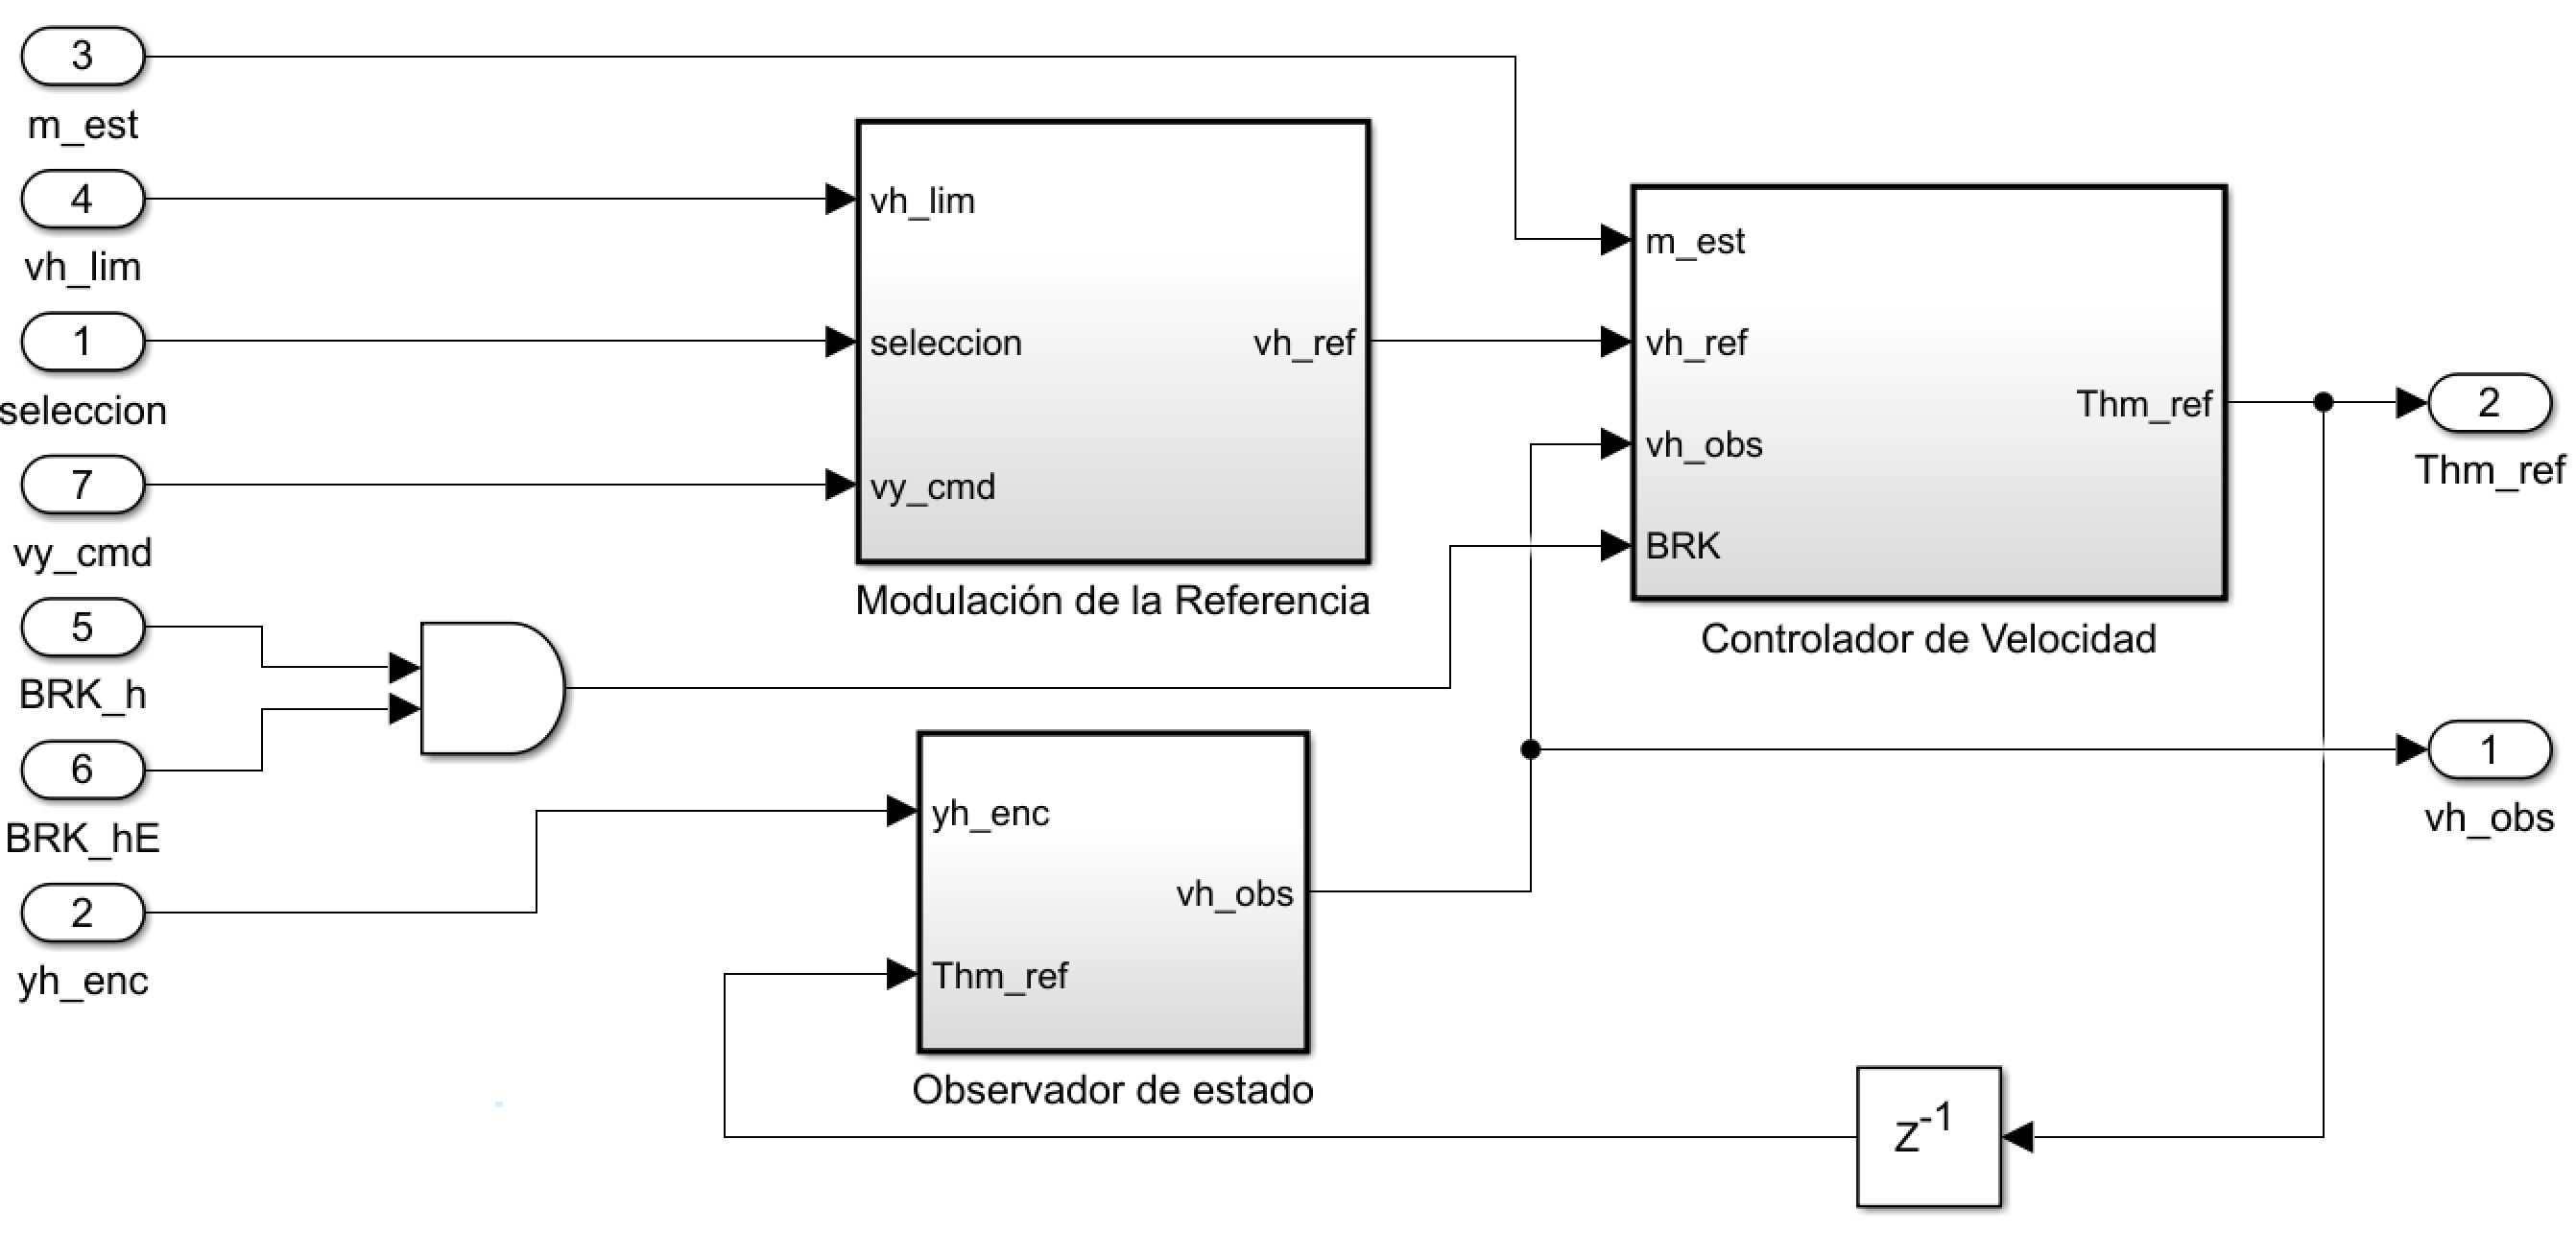
\includegraphics[width=1\textwidth]{control_izaje2.png}
    \caption{Control Regulatorio del Izaje (Hoist).}
\end{figure}
\begin{figure}[H]
    \centering
    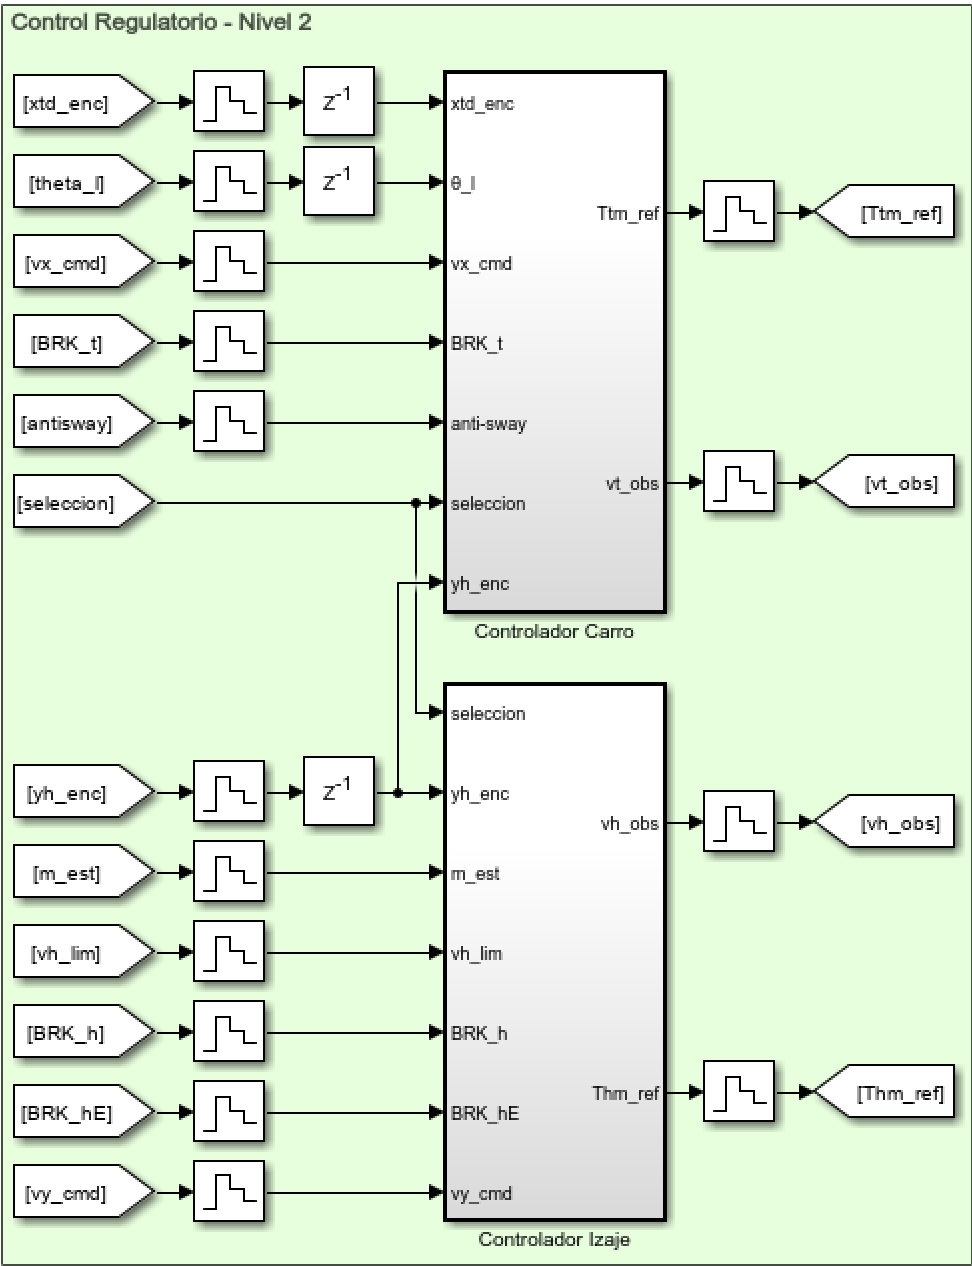
\includegraphics[width=0.8\textwidth]{control_regulatorio2.png}
    \caption{Modelo del Control Regulatorio en Simulink.}
\end{figure}

\section{Diseño del Control Supervisor (Nivel 1)}
El control supervisor actúa como el cerebro operativo de la grúa. Ejecutado a un tiempo de muestreo $T_{s1} = 20$ ms, su objetivo es tomar decisiones lógicas, garantizar la seguridad y coordinar los comandos que se envían al control regulatorio de bajo nivel. 

Para organizar esta lógica, la arquitectura se dividió en múltiples procesos paralelos, permitiendo que el control evalúe simultáneamente el modo de operación, la seguridad y el entorno.

\subsection{Autómata Principal de Modos de Operación}
Como primer bloque se desarrolla una máquina de estados. Este es el hilo de ejecución primario que dicta el comportamiento global de la grúa. Su objetivo es gestionar de manera segura las transiciones entre los distintos modos de operación:
\begin{itemize}
    \item \textbf{Stand By:} Estado de reposo y espera de comandos. Es el estado inicial del sistema, donde la grúa permanece con los frenos cerrados. Este estado también se activa automáticamente después de un período de inactividad o tras una operación completa, garantizando que la grúa no quede en una posición vulnerable.
    \item \textbf{Modo Manual:} Permite al operador tomar el control directo de las velocidades de los ejes a través del joystick. En conjunto con el bloque \textit{Manejo Cruceta} se encarga de traducir las señales del joystick en consignas de velocidad para el control regulatorio, permitiendo movimientos precisos y suaves. Este estado es activado siempre que se detecte una consigna en el joystick.
    \item \textbf{Modo Automático:} Es el estado más complejo, ya que debe controlar la grúa sin señales del operador. Incluye múltiples estados internos que permiten seleccionar el contenedor a mover. Luego toma el control de la grúa para mover el mismo desde un punto A hasta un punto B. A traves de dos funciones Matlab, genera una curva de movimiento segura, moviendo el spreader a estados intermedios que salen como consignas de velocidad al control regulatorio. Estas funciones manejan dos casos distintos: uno cuando no se conoce el perfil de obstáculos, el cual genera una trayectoria segura, y otro cuando sí se conoce, utilizando el mapa de alturas generado por el bloque paralelo de \textit{Índices y Perfil}.
    \item \textbf{Modos de Error y Recuperación:} En caso de detectarse una falla (propia del control supervisor o del control de seguridad), el autómata aborta cualquier operación actual y fuerza al sistema a adoptar una estado de resguardo para proteger la integridad de la carga y el equipo. Esto lo hace activando los frenos según corresponda. La recuperación se puede activar con el botón de reset, limitando la velocidad y dirección de movimiento manual. Una vez que el operador termina la maniobra de recuperación, puede volver al estado Stand By presionando el boton de reset nuevamente.
\end{itemize}
\begin{figure}[H]
    \centering
    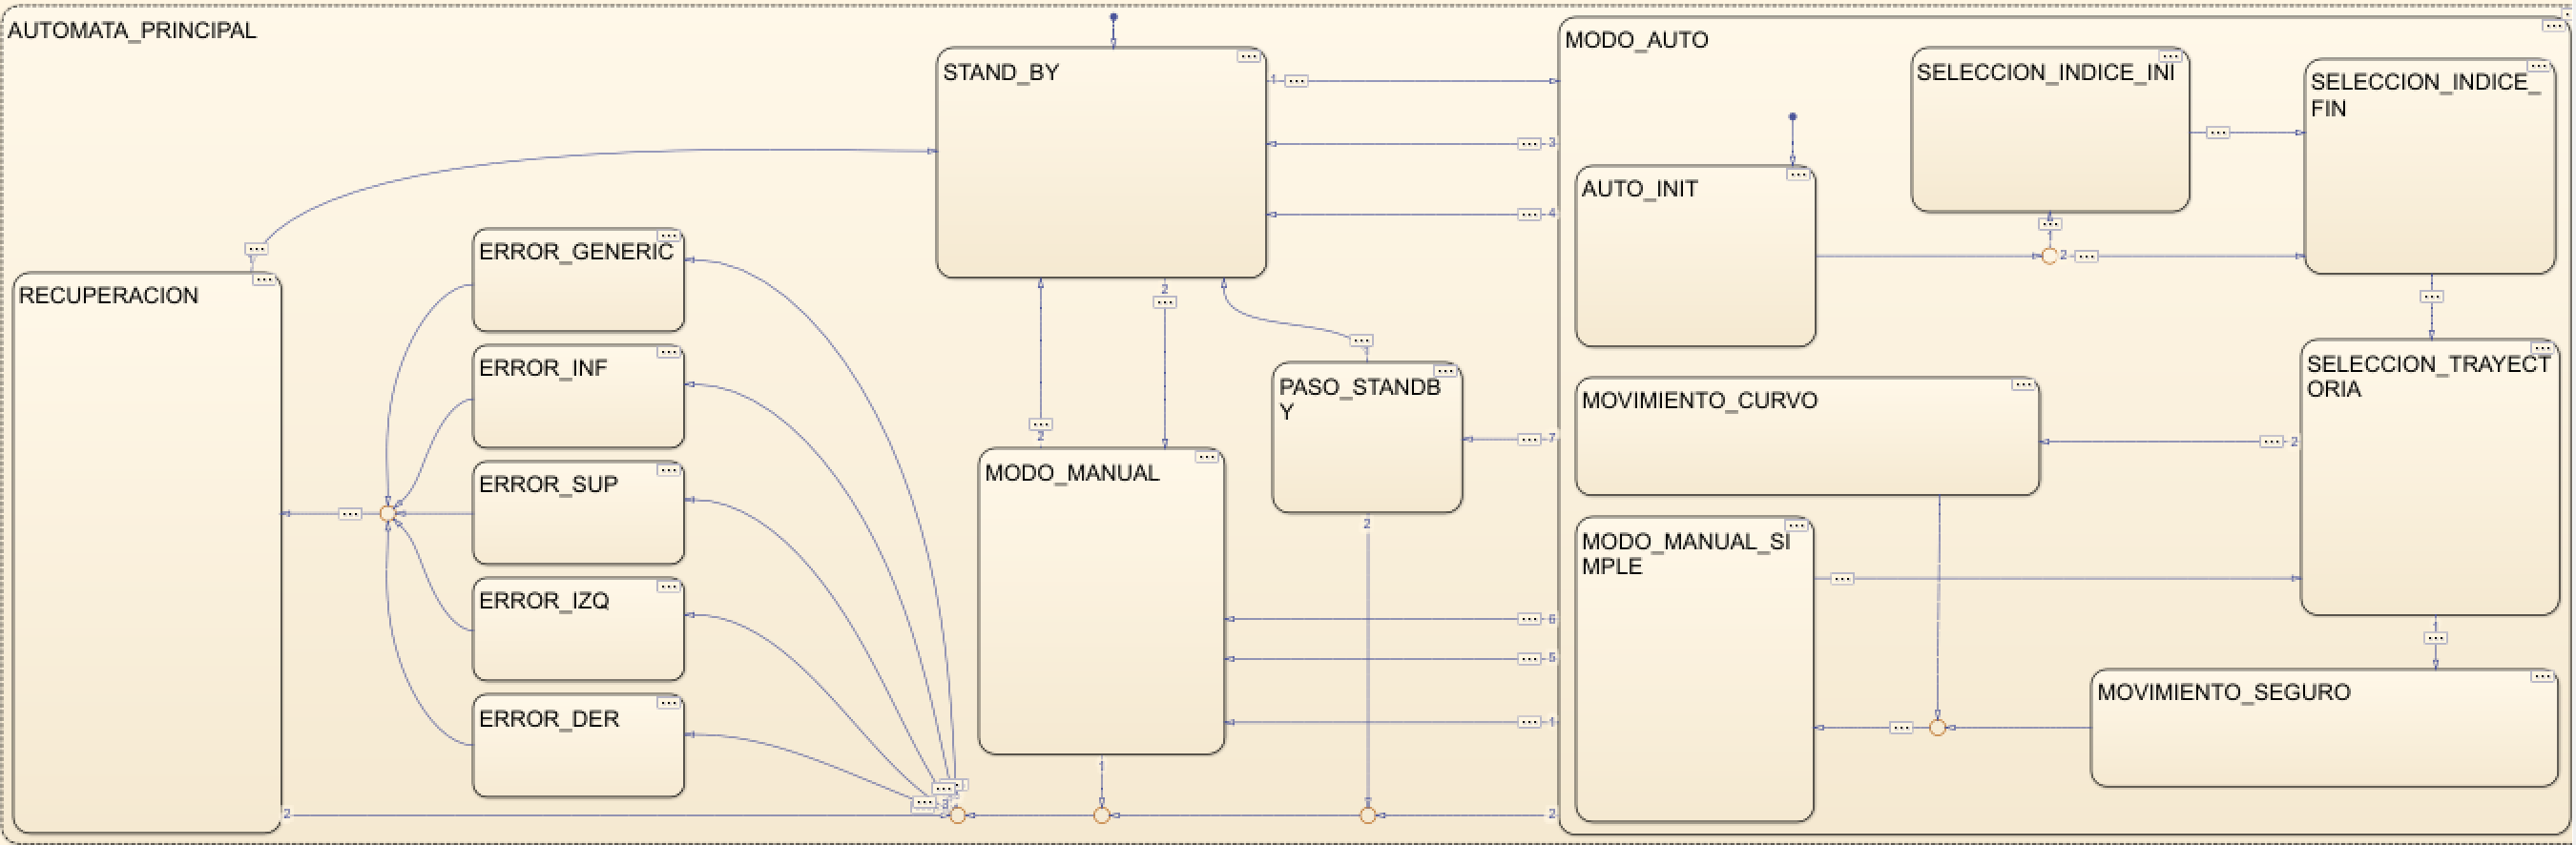
\includegraphics[width=1\textwidth]{automata_principal.png}
    \caption{Máquina de Estados en Stateflow.}
\end{figure}

\subsection{Gestión de Twistlocks}
Este bloque paralelo se encarga exclusivamente de la lógica del spreader. Administra los tiempos y las confirmaciones de los sensores para tomar (\texttt{CERRANDO\_TLK}) o soltar (\texttt{ABRIENDO\_TLK}) el contenedor, asegurando que la grúa nunca intente un movimiento de izaje si el anclaje no es mecánicamente seguro. Posee 4 estados internos: \texttt{VACIO}, estado inicial que mueve el spreader a la velocidad máxima permitida, \texttt{CERRANDO\_TLK}, que se activa cuando la tensión en el cable disminuye lo suficiente para indicar que el spreader se apoyó en un contenedor, \texttt{CARGADO}, que estima la masa del contenedor, limita la velocidad segun la curva de potencia y detecta sobrecarga, y \texttt{ABRIENDO\_TLK}, que análogamente al estado de cerrar, detecta que la tensión disminuya para abrir los twistlocks. Finalmente se transiciona al estado inicial una vez superada cierta altura de seguridad.
\begin{figure}[H]
    \centering
    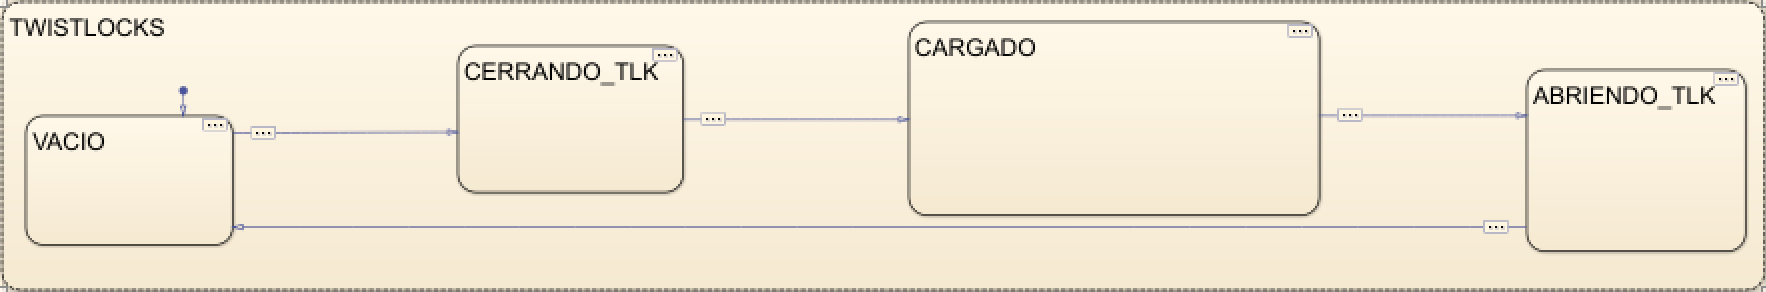
\includegraphics[width=1\textwidth]{twistlocks.png}
    \caption{Lógica Twistlocks en Stateflow.}
\end{figure}

\subsection{Suavizador de Consignas de Velocidad}
Se encarga de aplicar filtros de suavizado a las consignas de velocidad provenientes del autómata principal. Esto es especialmente importante en el modo manual, donde las señales del joystick pueden ser abruptas. El bloque implementa límites de jerk, aceleración y velocidad, garantizando que cualquier cambio en la referencia se realice de manera gradual, evitando movimientos bruscos que puedan comprometer la estabilidad o seguridad de la operación.
\begin{figure}[H]
    \centering
    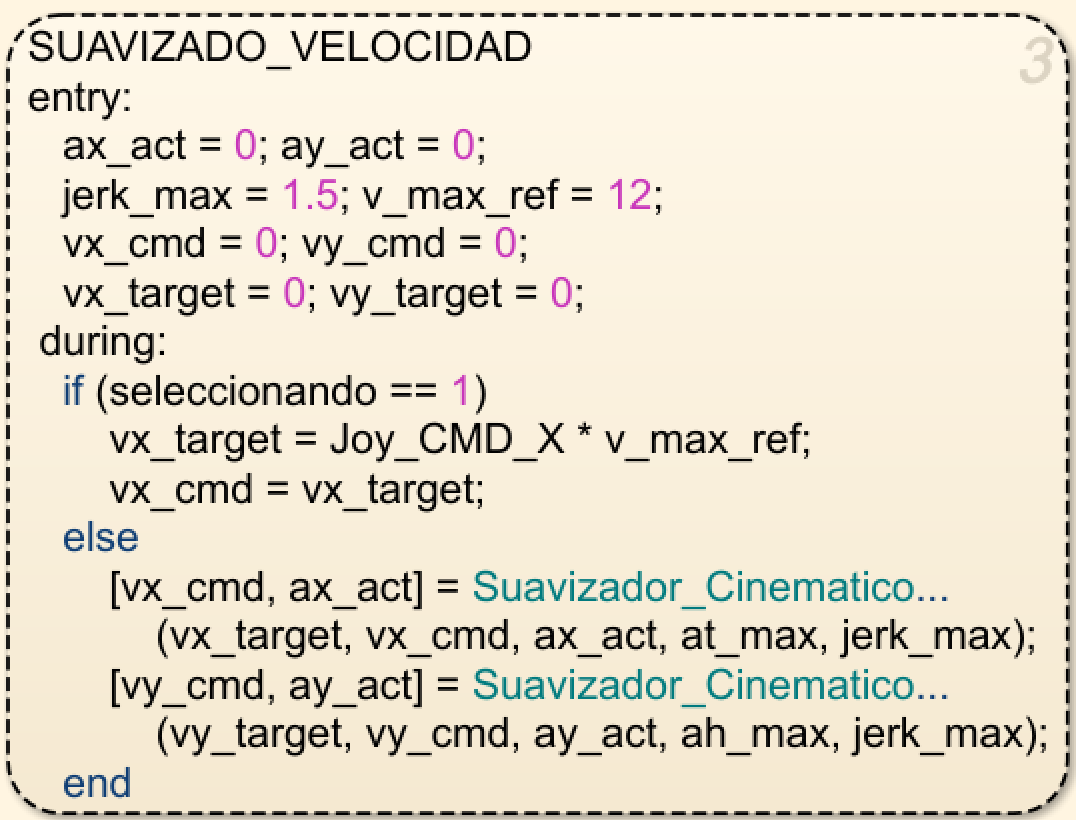
\includegraphics[width=0.55\textwidth]{suavizado_vel.png}
    \caption{Suavizador de Velocidad.}
\end{figure}

\subsection{Análisis Espacial, Perfil de Obstáculos y Actualización de Cruceta}
Para que el modo automático pueda trazar rutas seguras, la grúa debe conocer su entorno. Este bloque procesa los datos de los sensores de escaneo del LIDAR y actualiza continuamente un mapa de alturas o perfil de obstáculos bajo el área de trabajo. Esto garantiza que cualquier trayectoria generada esquive las pilas de contenedores existentes. Al mismo tiempo, calcula los índices en los que se encuentra el carro. El perfil de alturas se representa como una envolvente de seguridad, con margenes laterales y superiores que garantizan que la grúa no intente pasar por zonas donde pueda colisionar con obstáculos. Por último, también se encarga de actualizar la posición de la cruceta, que es el punto de referencia para el operador, asegurando que siempre se muestre la posición real del spreader en la interfaz.
\begin{figure}[H]
    \centering
    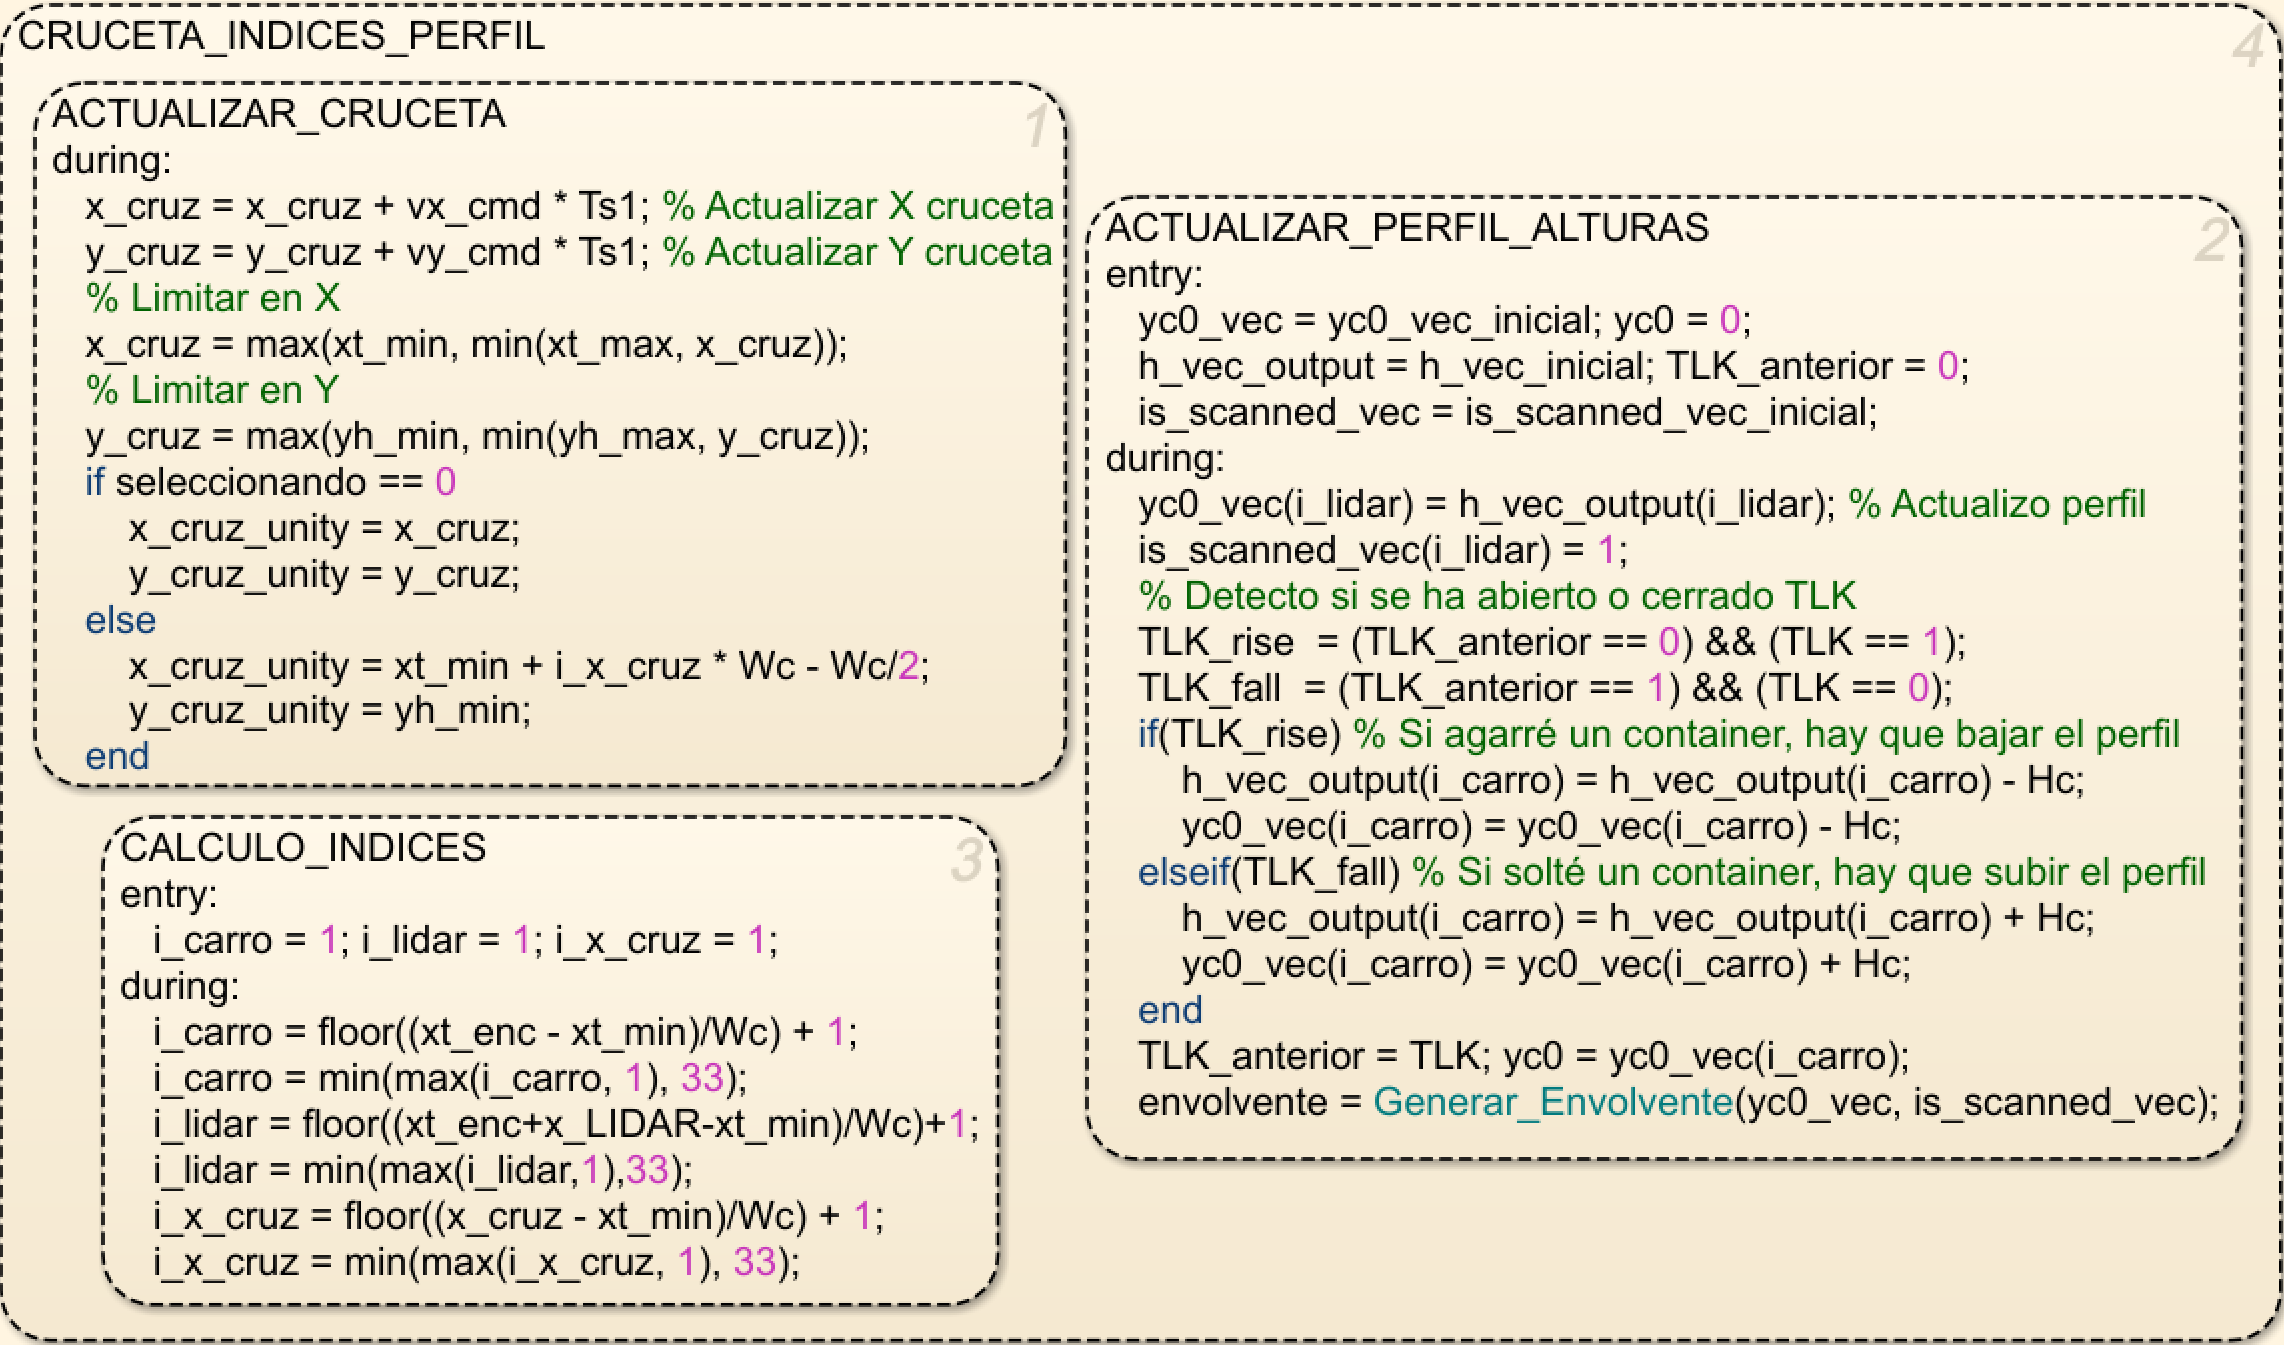
\includegraphics[width=1\textwidth]{cruz_ind_perfil.png}
    \caption{Índices y Perfil de Obstáculos en Stateflow.}
\end{figure}

\subsection{Supervisión de Comunicación (Watchdog Heartbeat)}
Este bloque constituye un anillo de seguridad vital. Se encarga de emitir pulsos de vida (\textit{heartbeats}) a intervalos regulares. En el control de seguridad, otro bloque observa esta señal. Si se detecta una falta de pulsos (superando un tiempo preestablecido), el sistema de seguridad asume una pérdida de comunicación, interrumpiendo cualquier movimiento en curso y envíando al sistema al estado de error.
\begin{figure}[H]
    \centering
    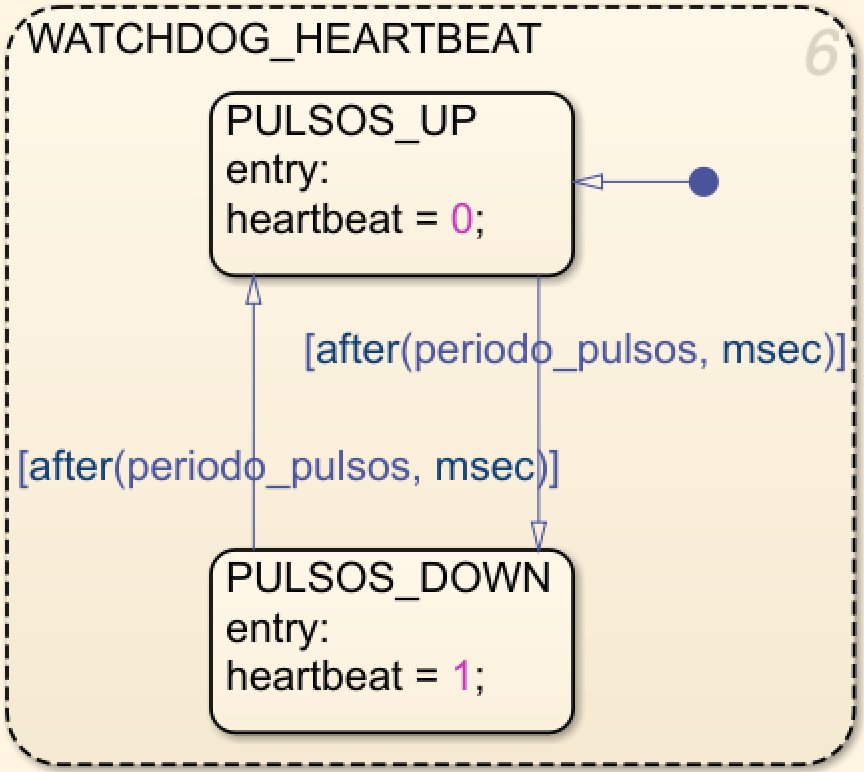
\includegraphics[width=0.4\textwidth]{watchdog_heartbeat.png}
    \caption{Watchdog Heartbeat en Stateflow.}
\end{figure}

\subsection{Límites Suaves}
Este bloque de código actúa como una barrera de seguridad preventiva. Antes de que el carro o el izaje alcancen los límites físicos extremos de su carrera (donde actuarían los finales de carrera), este bloque recorta gradualmente las referencias de velocidad, forzando una detención suave y controlada dentro del área de trabajo válida.

\subsection{Modelo del Control Supervisor en Simulink}
\begin{figure}[H]
    \centering
    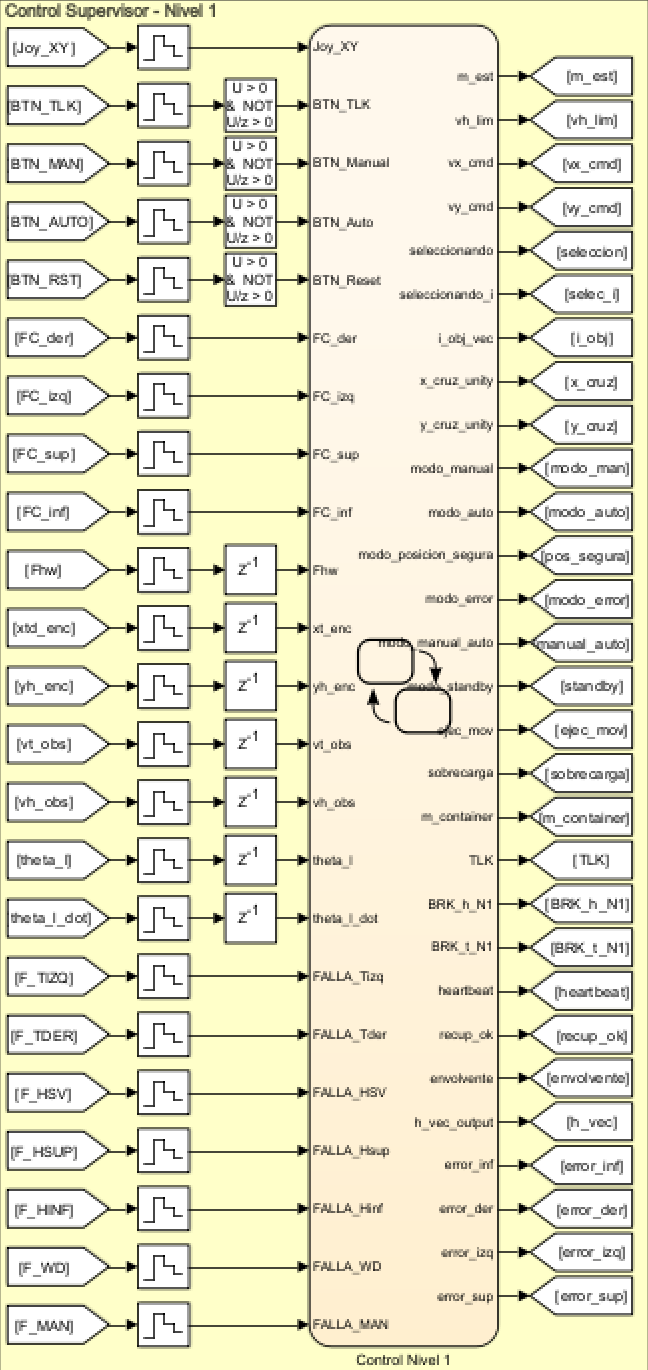
\includegraphics[width=0.66\textwidth]{control_supervisor2.png}
    \caption{Modelo del Control Supervisor en Simulink.}
\end{figure}

\subsection{Control del Joystick y Botones Físicos}
Para controlar la grúa, se utiliza un joystick físico conectado a la estación de operación. Este dispositivo permite al operador controlar directamente las velocidades de traslación e izaje, así como activar comandos específicos (como el cierre de twistlocks). El bloque de manejo de entradas en el control supervisor procesa estas señales para generar referencias adecuadas para el control regulatorio.
\begin{figure}[H]
    \centering
    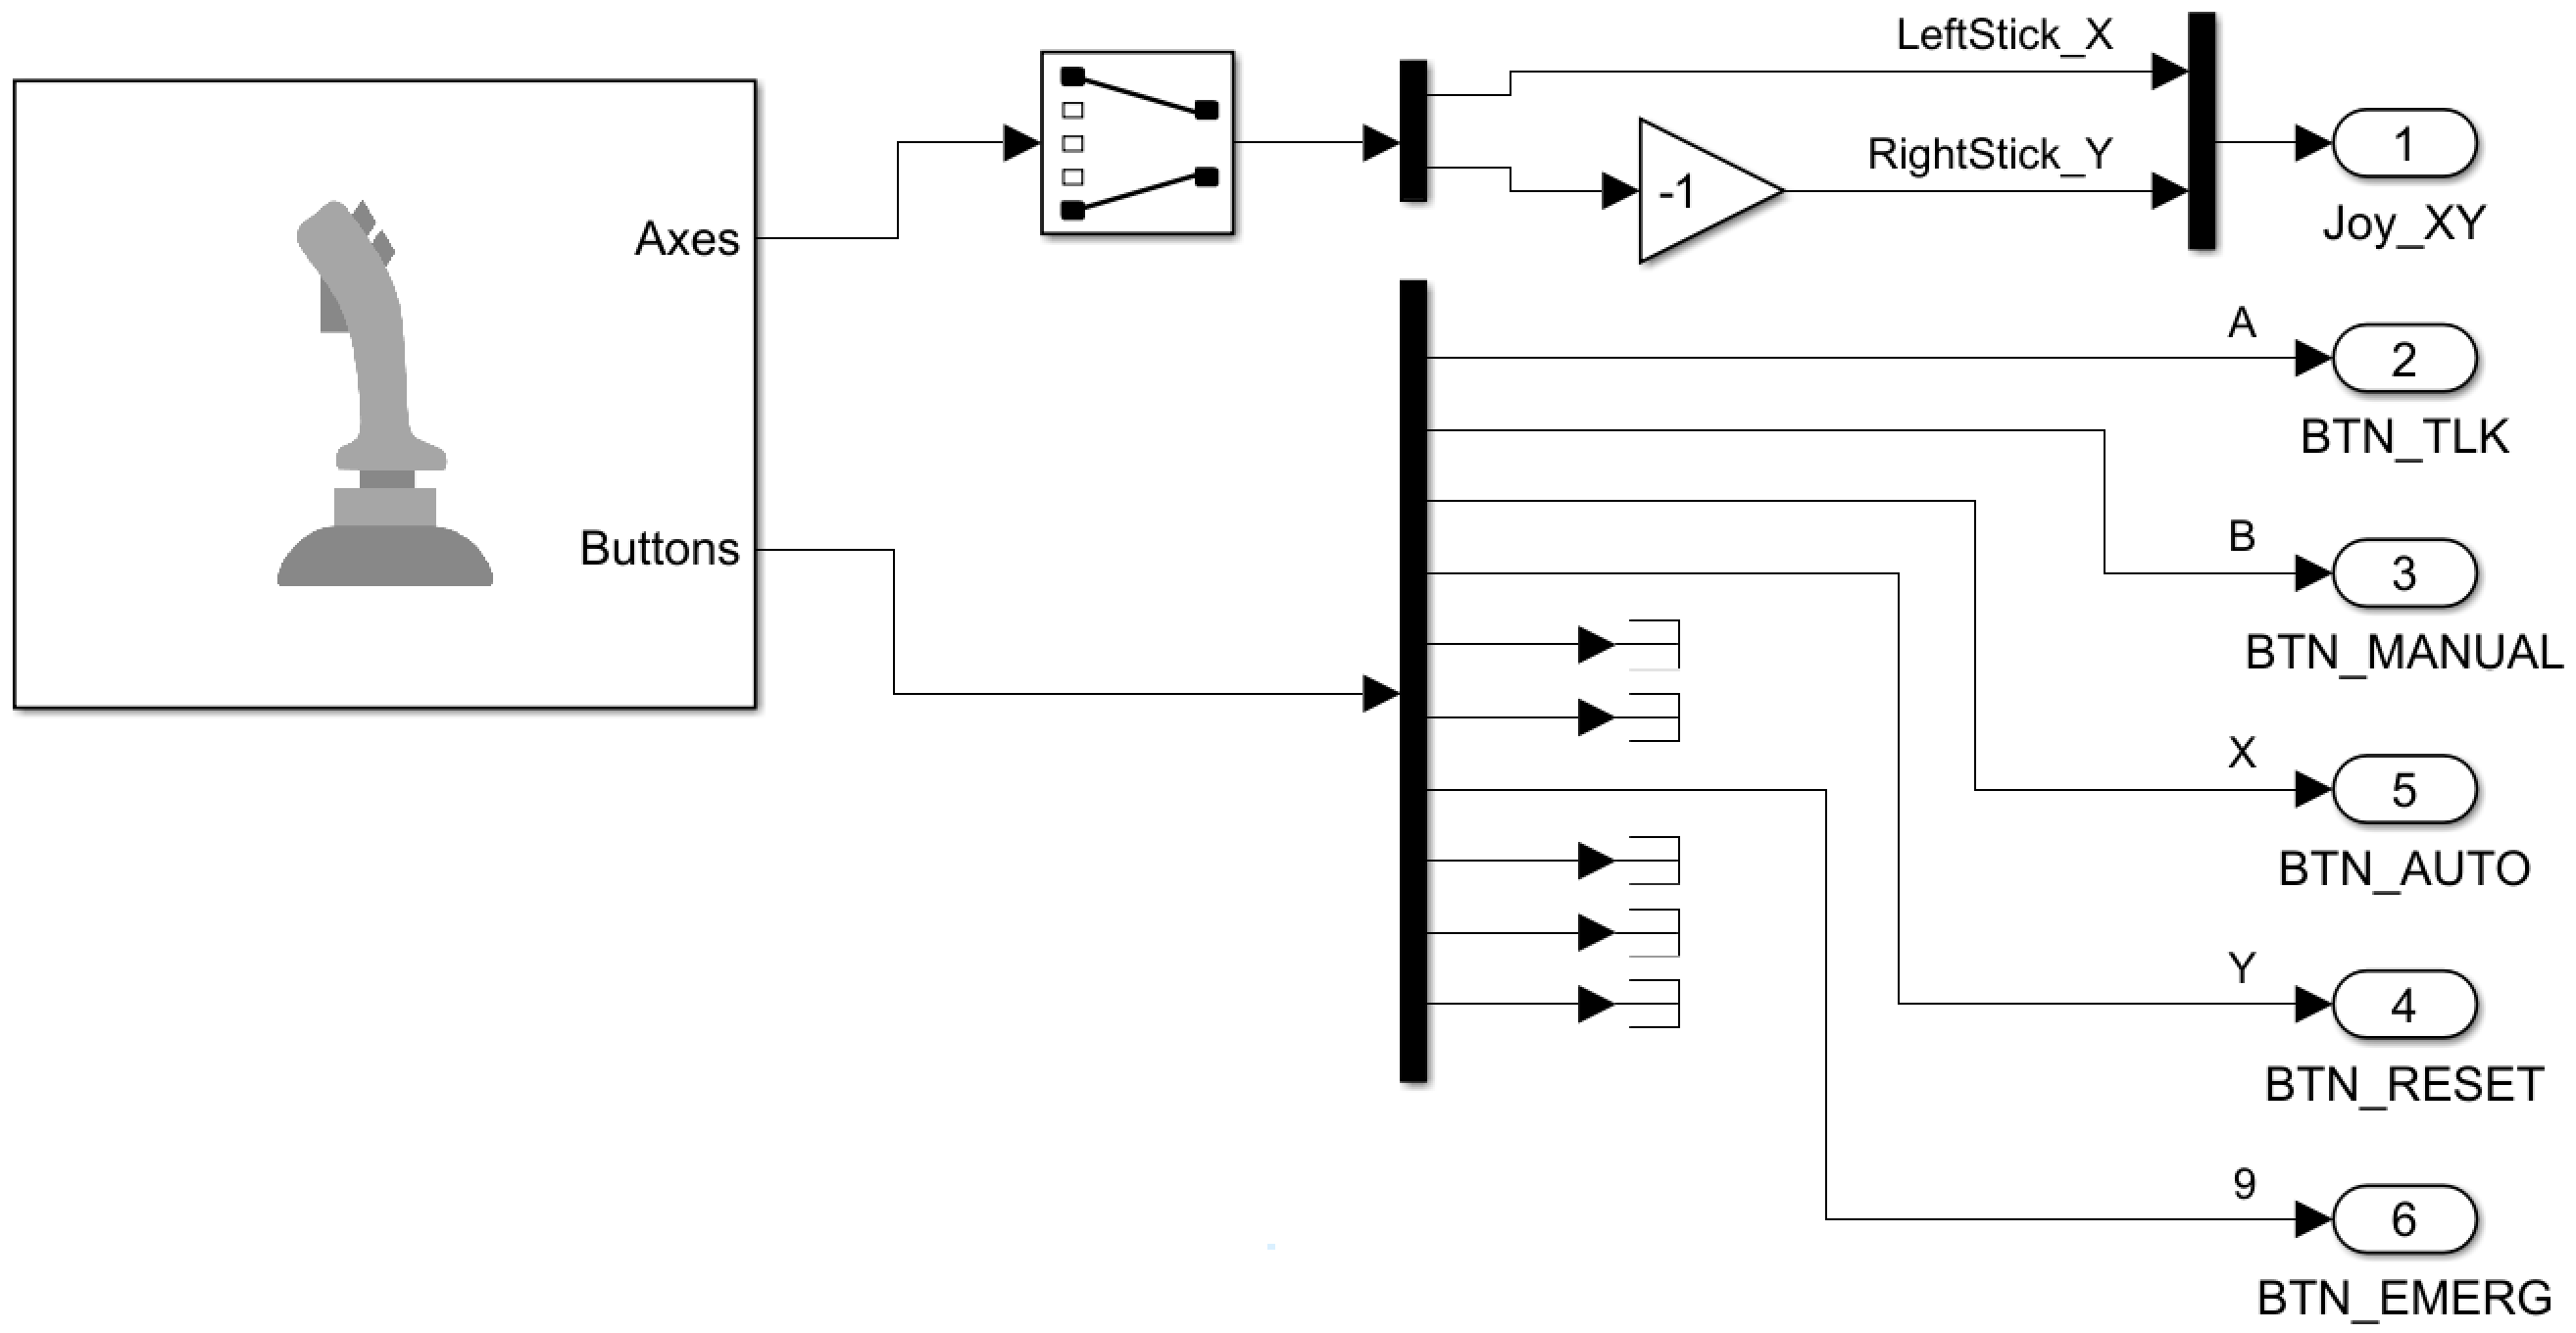
\includegraphics[width=1\textwidth]{joystick.png}
    \caption{Bloque de Configuración del Joystick en Stateflow.}
\end{figure}

\section{Diseño del Control de Seguridad (Nivel 0)}
El Nivel 0 representa la capa de protección más baja y con mayor jerarquía dentro de la arquitectura de control. Su función exclusiva es salvaguardar la integridad de la grúa, la carga y el personal. Este nivel tiene la autoridad para sobrescribir cualquier comando proveniente del Nivel 1, cortando la energía de los actuadores y aplicando los frenos mecánicos ante cualquier anomalía. 

La lógica de seguridad se modeló mediante dos procesos paralelos continuos:

\subsection{MAutómata de Estados de Seguridad}
Esta máquina de estados supervisa constantemente el estado físico de la máquina a través de la redundancia de sensores. Durante la operación normal, el sistema permanece en el estado \texttt{SISTEMA\_OK}. 

Dentro de este estado nominal, el bloque realiza un cálculo dinámico crítico: ajusta en tiempo real el límite de velocidad de izaje permitido ($vh\_lim$) en función de la masa actual de la carga. Esto garantiza que el motor nunca exceda su potencia nominal ($P_{nom}$), comportándose según una curva de potencia constante (sobrevelocidad).

El sistema evaluará continuamente condiciones de falla para transicionar a estados de emergencia específicos, en los cuales se aplican inmediatamente los frenos de emergencia ($BRK_{t} = 0$, $BRK_{hE} = 0$), según corresponda:
\begin{itemize}
    \item \textbf{Emergencia de Izaje:} Se activa uno de los 3 estados según corresponda: si la velocidad observada supera en un $15\%$ al límite dinámico calculado (sobrevelocidad), si se activan los finales de carrera superior/inferior (\texttt{FCE\_sup}, \texttt{FCE\_inf}).
    \item \textbf{Emergencia de Carro:} Se activa uno de los 2 estados: si el carro activa los finales de carrera extremos (\texttt{FCE\_izq}, \texttt{FCE\_der}).
    \item \textbf{Emergencia Manual:} Detención forzada accionada por el operador mediante el botón físico de emergencia (\texttt{BTN\_Emerg}).
    \item \textbf{Emergencia de Comunicación (\texttt{EMERGENCIA\_WD}):} Disparada por la pérdida de comunicación con el control supervisor, utilizando el watchdog.
\end{itemize}

Una vez mitigada la causa de la parada, el sistema exige un rearme manual (\texttt{BTN\_Reset}) que hace transicionar a la máquina a un \texttt{MODO\_RECUPERACION} antes de permitir volver a operación nominal.
\begin{figure}[H]
    \centering
    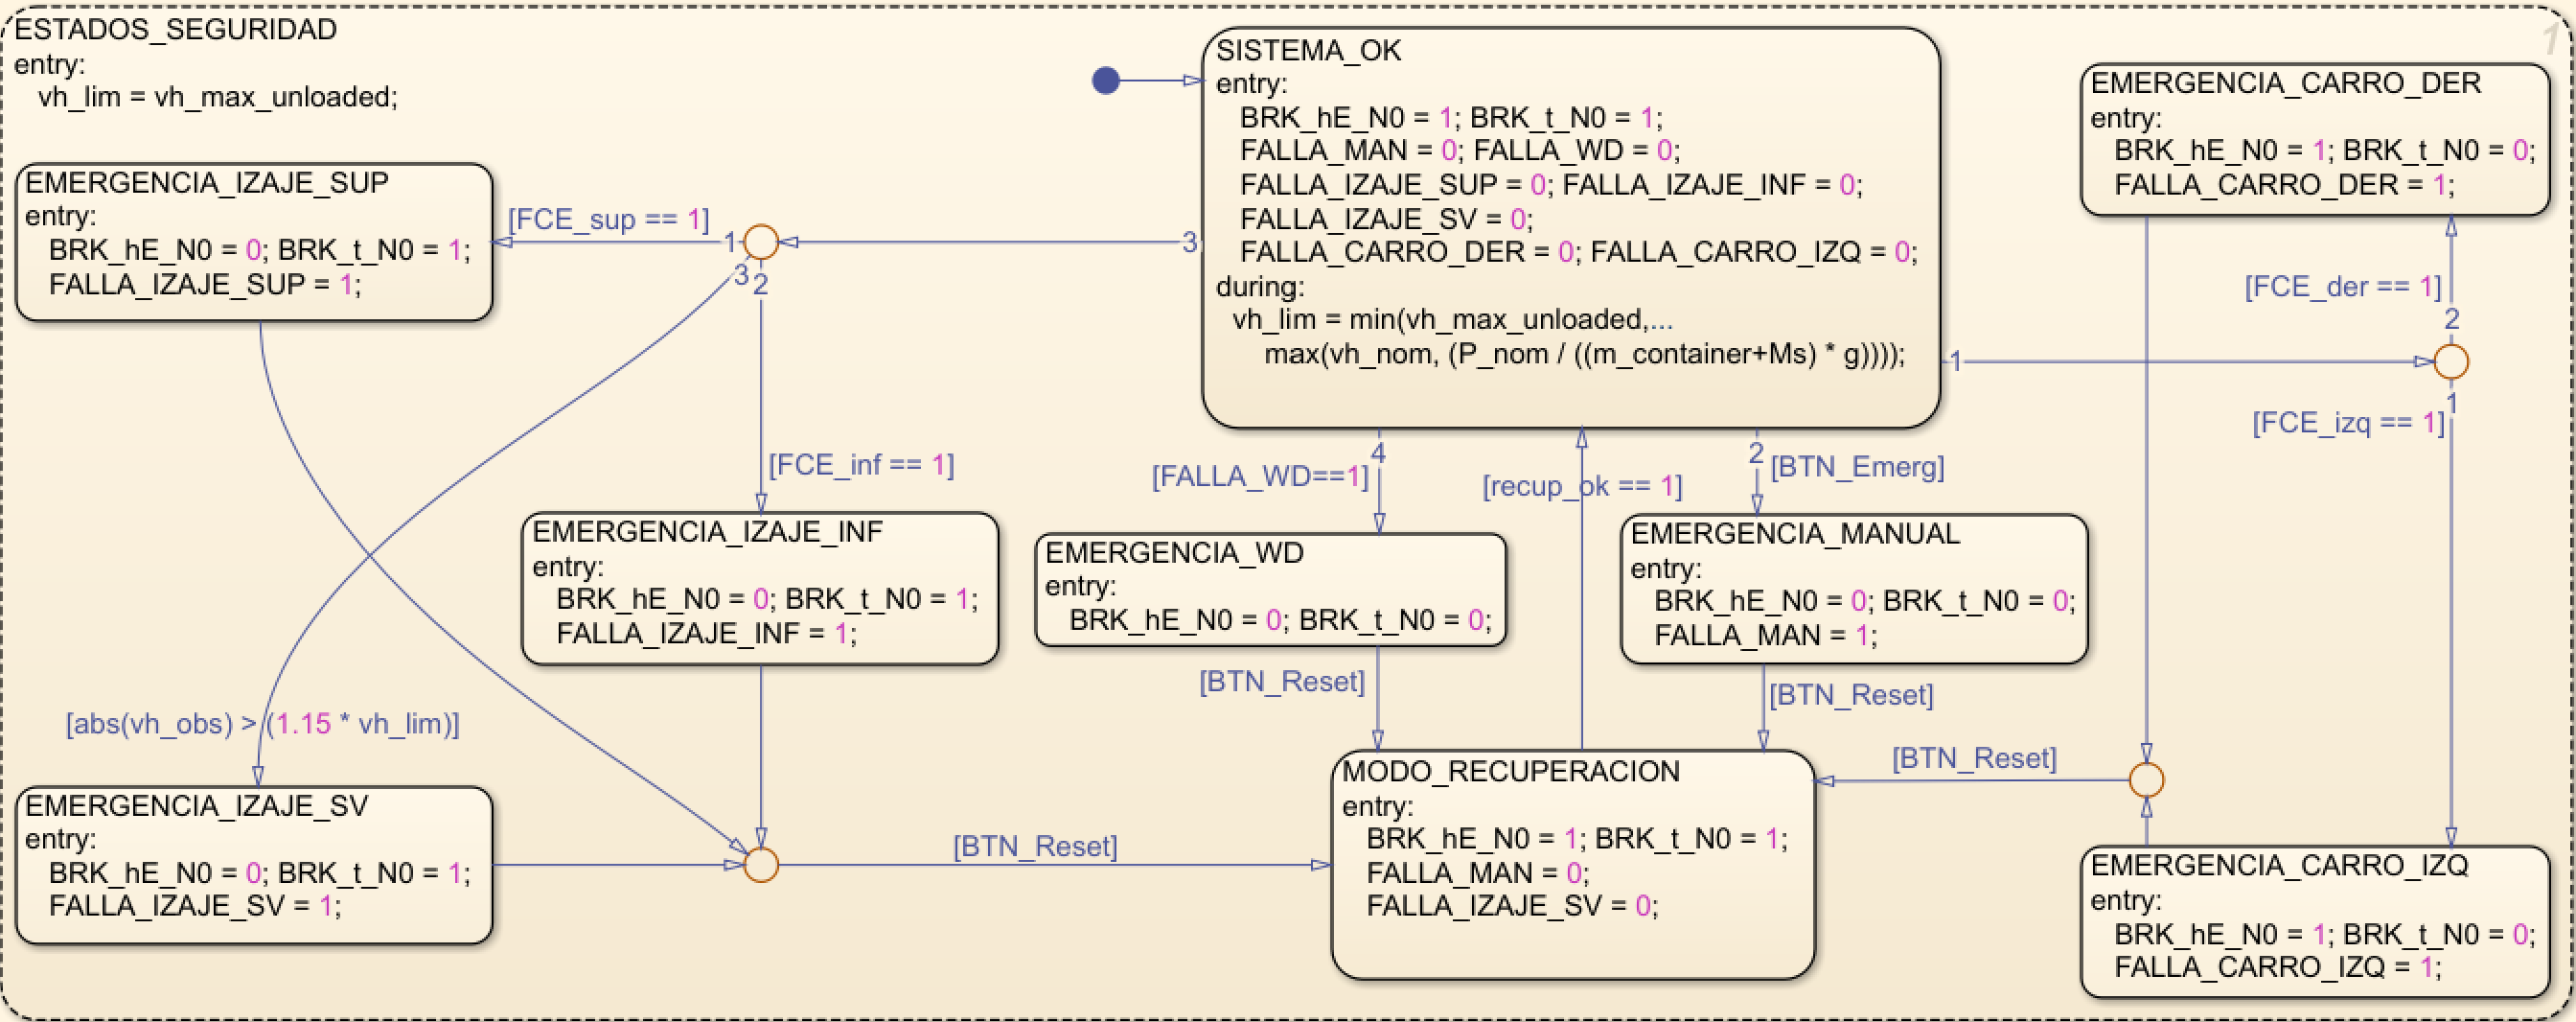
\includegraphics[width=1\textwidth]{automata_seguridad.png}
    \caption{Estados de Seguridad en Stateflow.}
\end{figure}

\subsection{Monitor de Comunicaciones}
Este segundo proceso paralelo funciona como un supervisor de la integridad de la red de datos. El control supervisor debe enviar una señal de latido (\textit{heartbeat}) que alterna su estado constantemente. 

La máquina de estados del Watchdog alterna entre \texttt{HEARTBEAT\_DOWN} y \texttt{HEARTBEAT\_UP} persiguiendo esta señal. Si la señal se congela y el sistema permanece en un solo estado por una cantidad de ciclos de reloj que supere el límite seguro (\texttt{counter\_limit}), se declara una falla de red (\texttt{FALLA\_WD}), lo que dispara la parada de emergencia en el proceso principal para evitar que la grúa continúe moviéndose con el último comando recibido.
\begin{figure}[H]
    \centering
    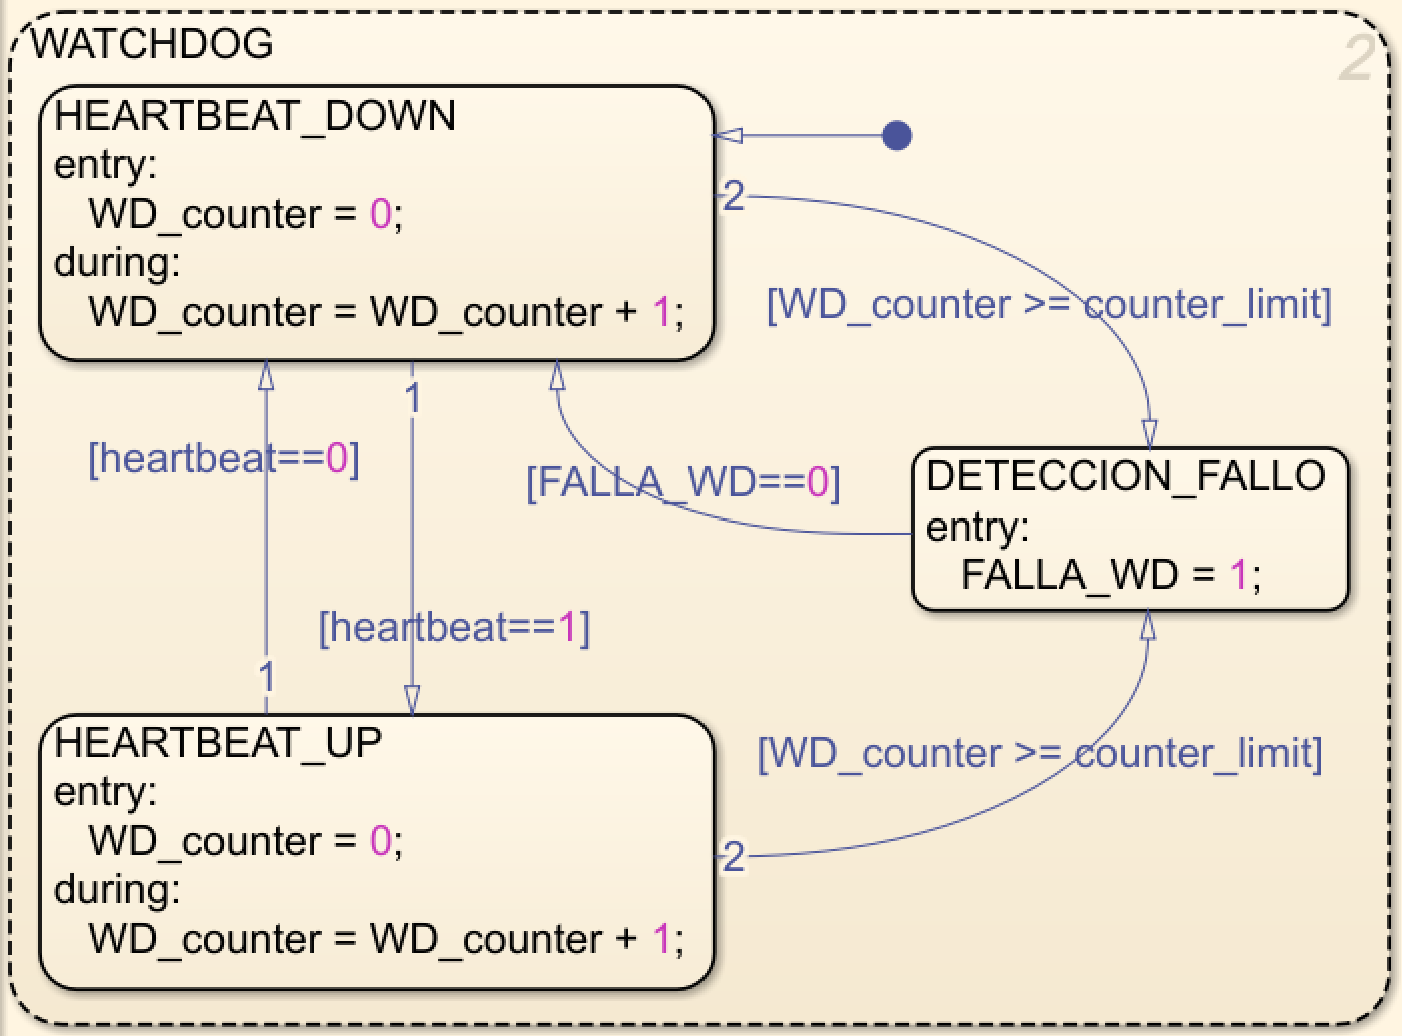
\includegraphics[width=0.55\textwidth]{watchdog.png}
    \caption{Watchdog en Stateflow.}
\end{figure}

\subsection{Modelo del Control de Seguridad en Simulink}
\begin{figure}[H]
    \centering
    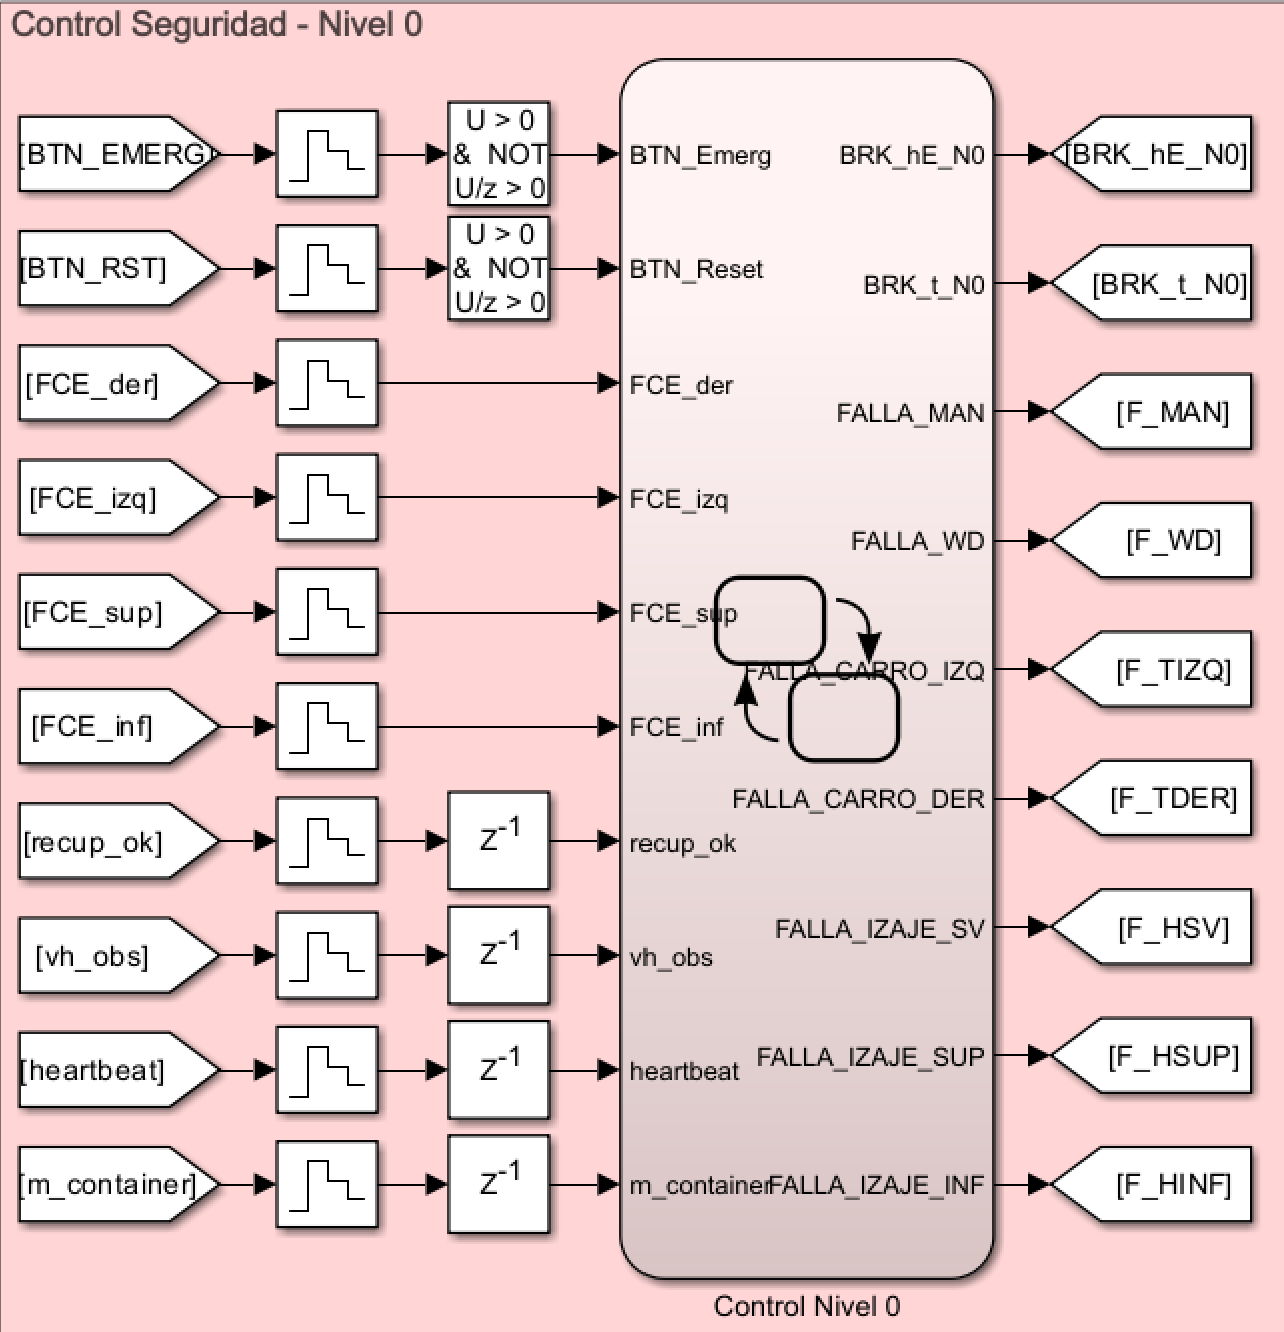
\includegraphics[width=0.8\textwidth]{control_seguridad2.png}
    \caption{Modelo del Control de Seguridad en Simulink.}
\end{figure}

\section{Comunicación y Animación con Unity}
Para la visualización en tiempo real de la grúa y su entorno, se implementó un bloque de comunicación que transmite los estados críticos del sistema a una aplicación desarrollada en Unity. Esta aplicación renderiza una representación 2D de la grúa, los contenedores y el barco, permitiendo al operador monitorear visualmente la operación.
\begin{figure}[H]
    \centering
    \begin{subfigure}{0.39\textwidth}
        \centering
        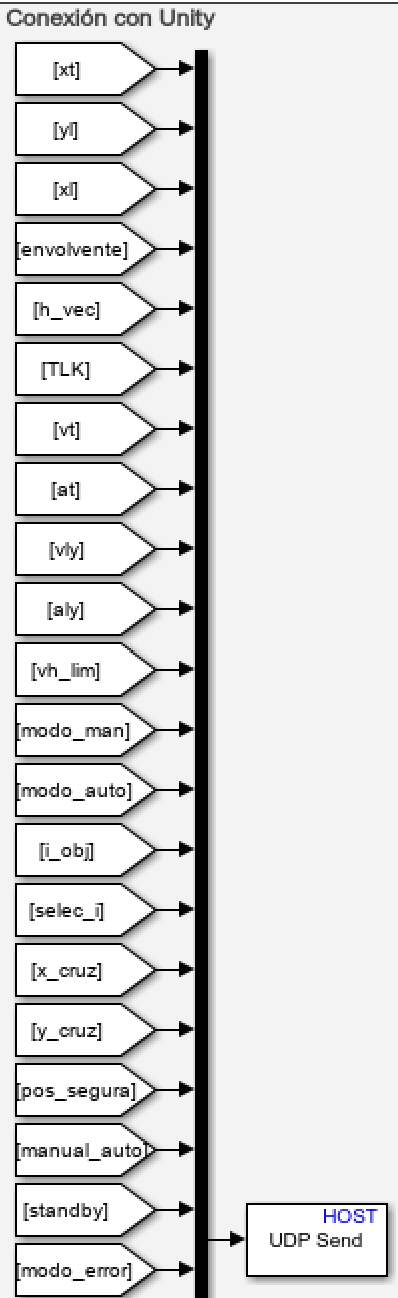
\includegraphics[width=\linewidth]{unity11.png}
    \end{subfigure}
    \hfill
    \begin{subfigure}{0.39\textwidth}
        \centering
        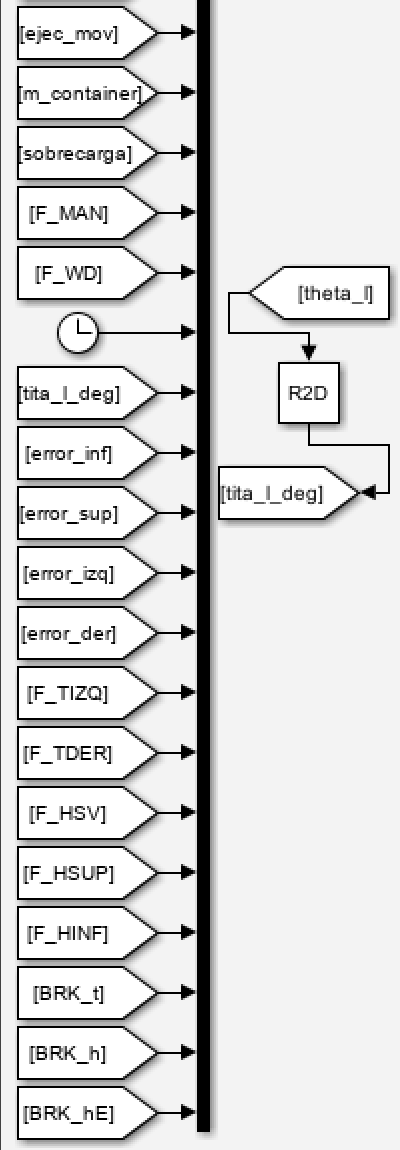
\includegraphics[width=\linewidth]{unity22.png}
    \end{subfigure}
    \caption{Bloque de Comunicación con Unity en Simulink.}
\end{figure}

A continuación se presentan algunas capturas en diferentes estados de la grúa, mostrando la posición del spreader, la carga y el entorno. Estas visualizaciones son fundamentales para que el operador tenga una referencia clara de la operación en curso, especialmente en modo automático.
\begin{figure}[H]
    \centering
    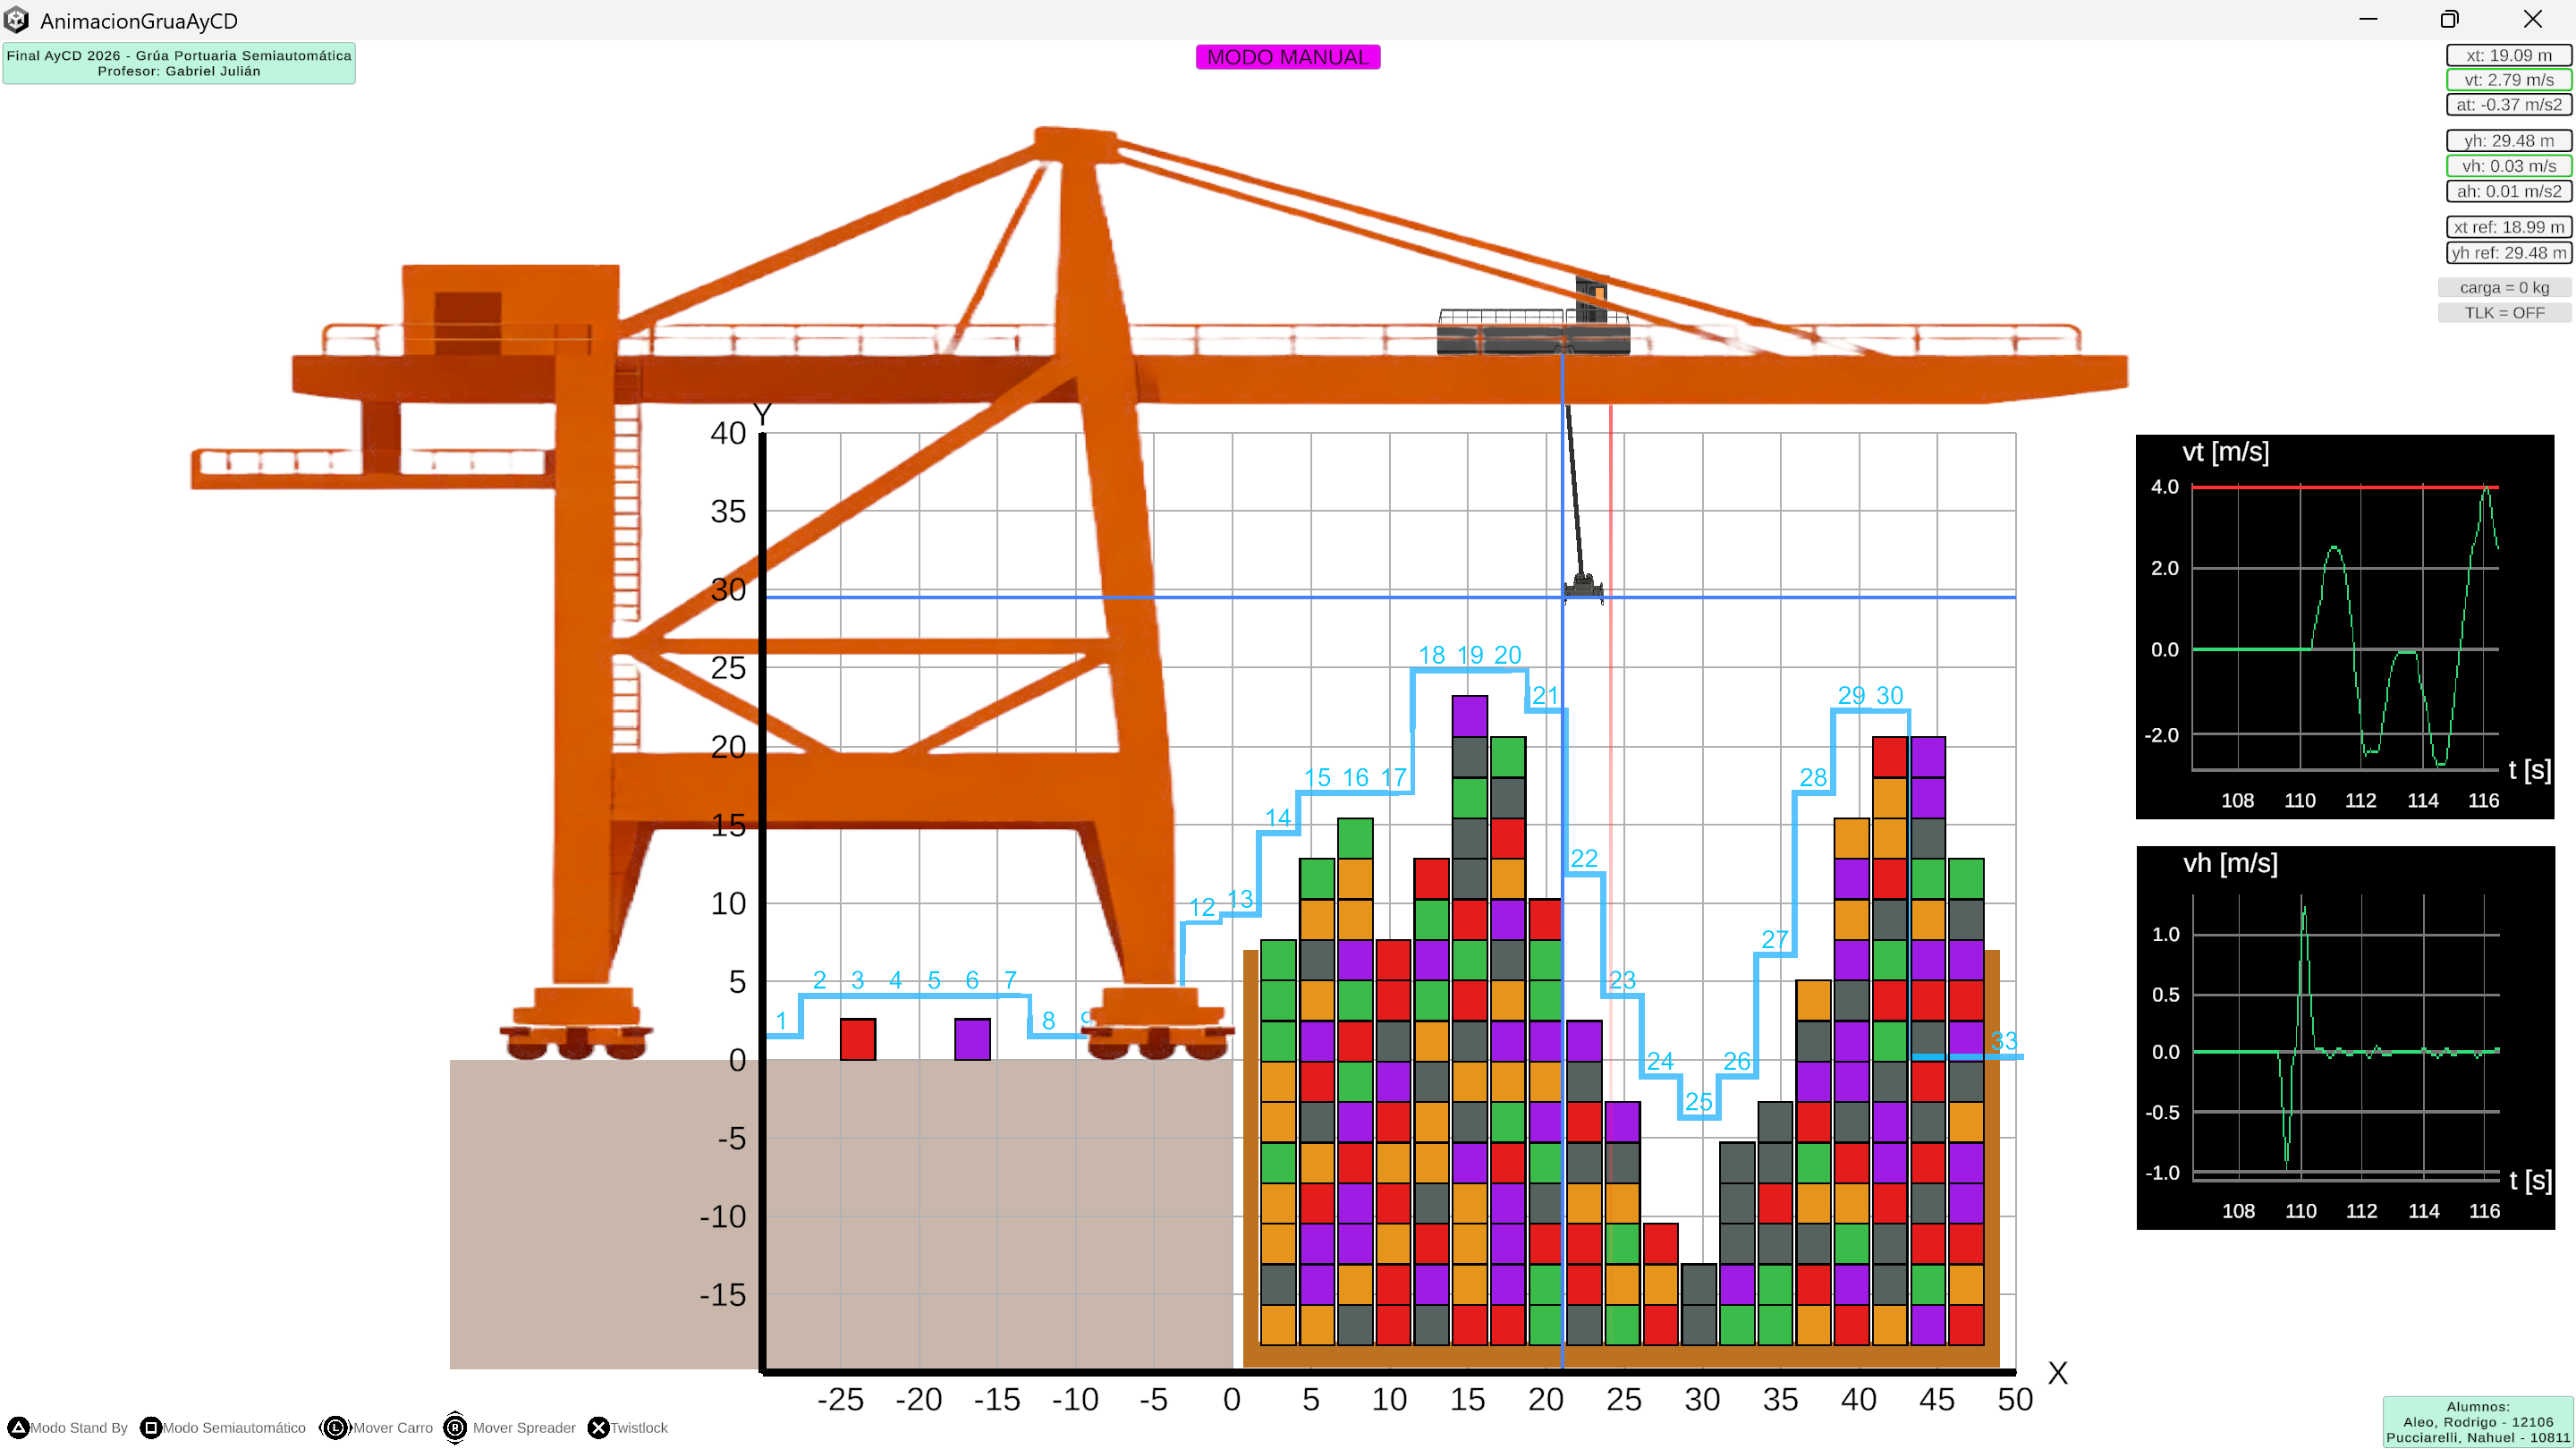
\includegraphics[width=1\textwidth]{unity_grua1.png}
    \caption{Modo Manual. Nótese la envolvente de seguridad del perfil de obstáculos y la zona aún sin medir con el LIDAR (índice 31 en adelante).}
\end{figure}
\begin{figure}[H]
    \centering
    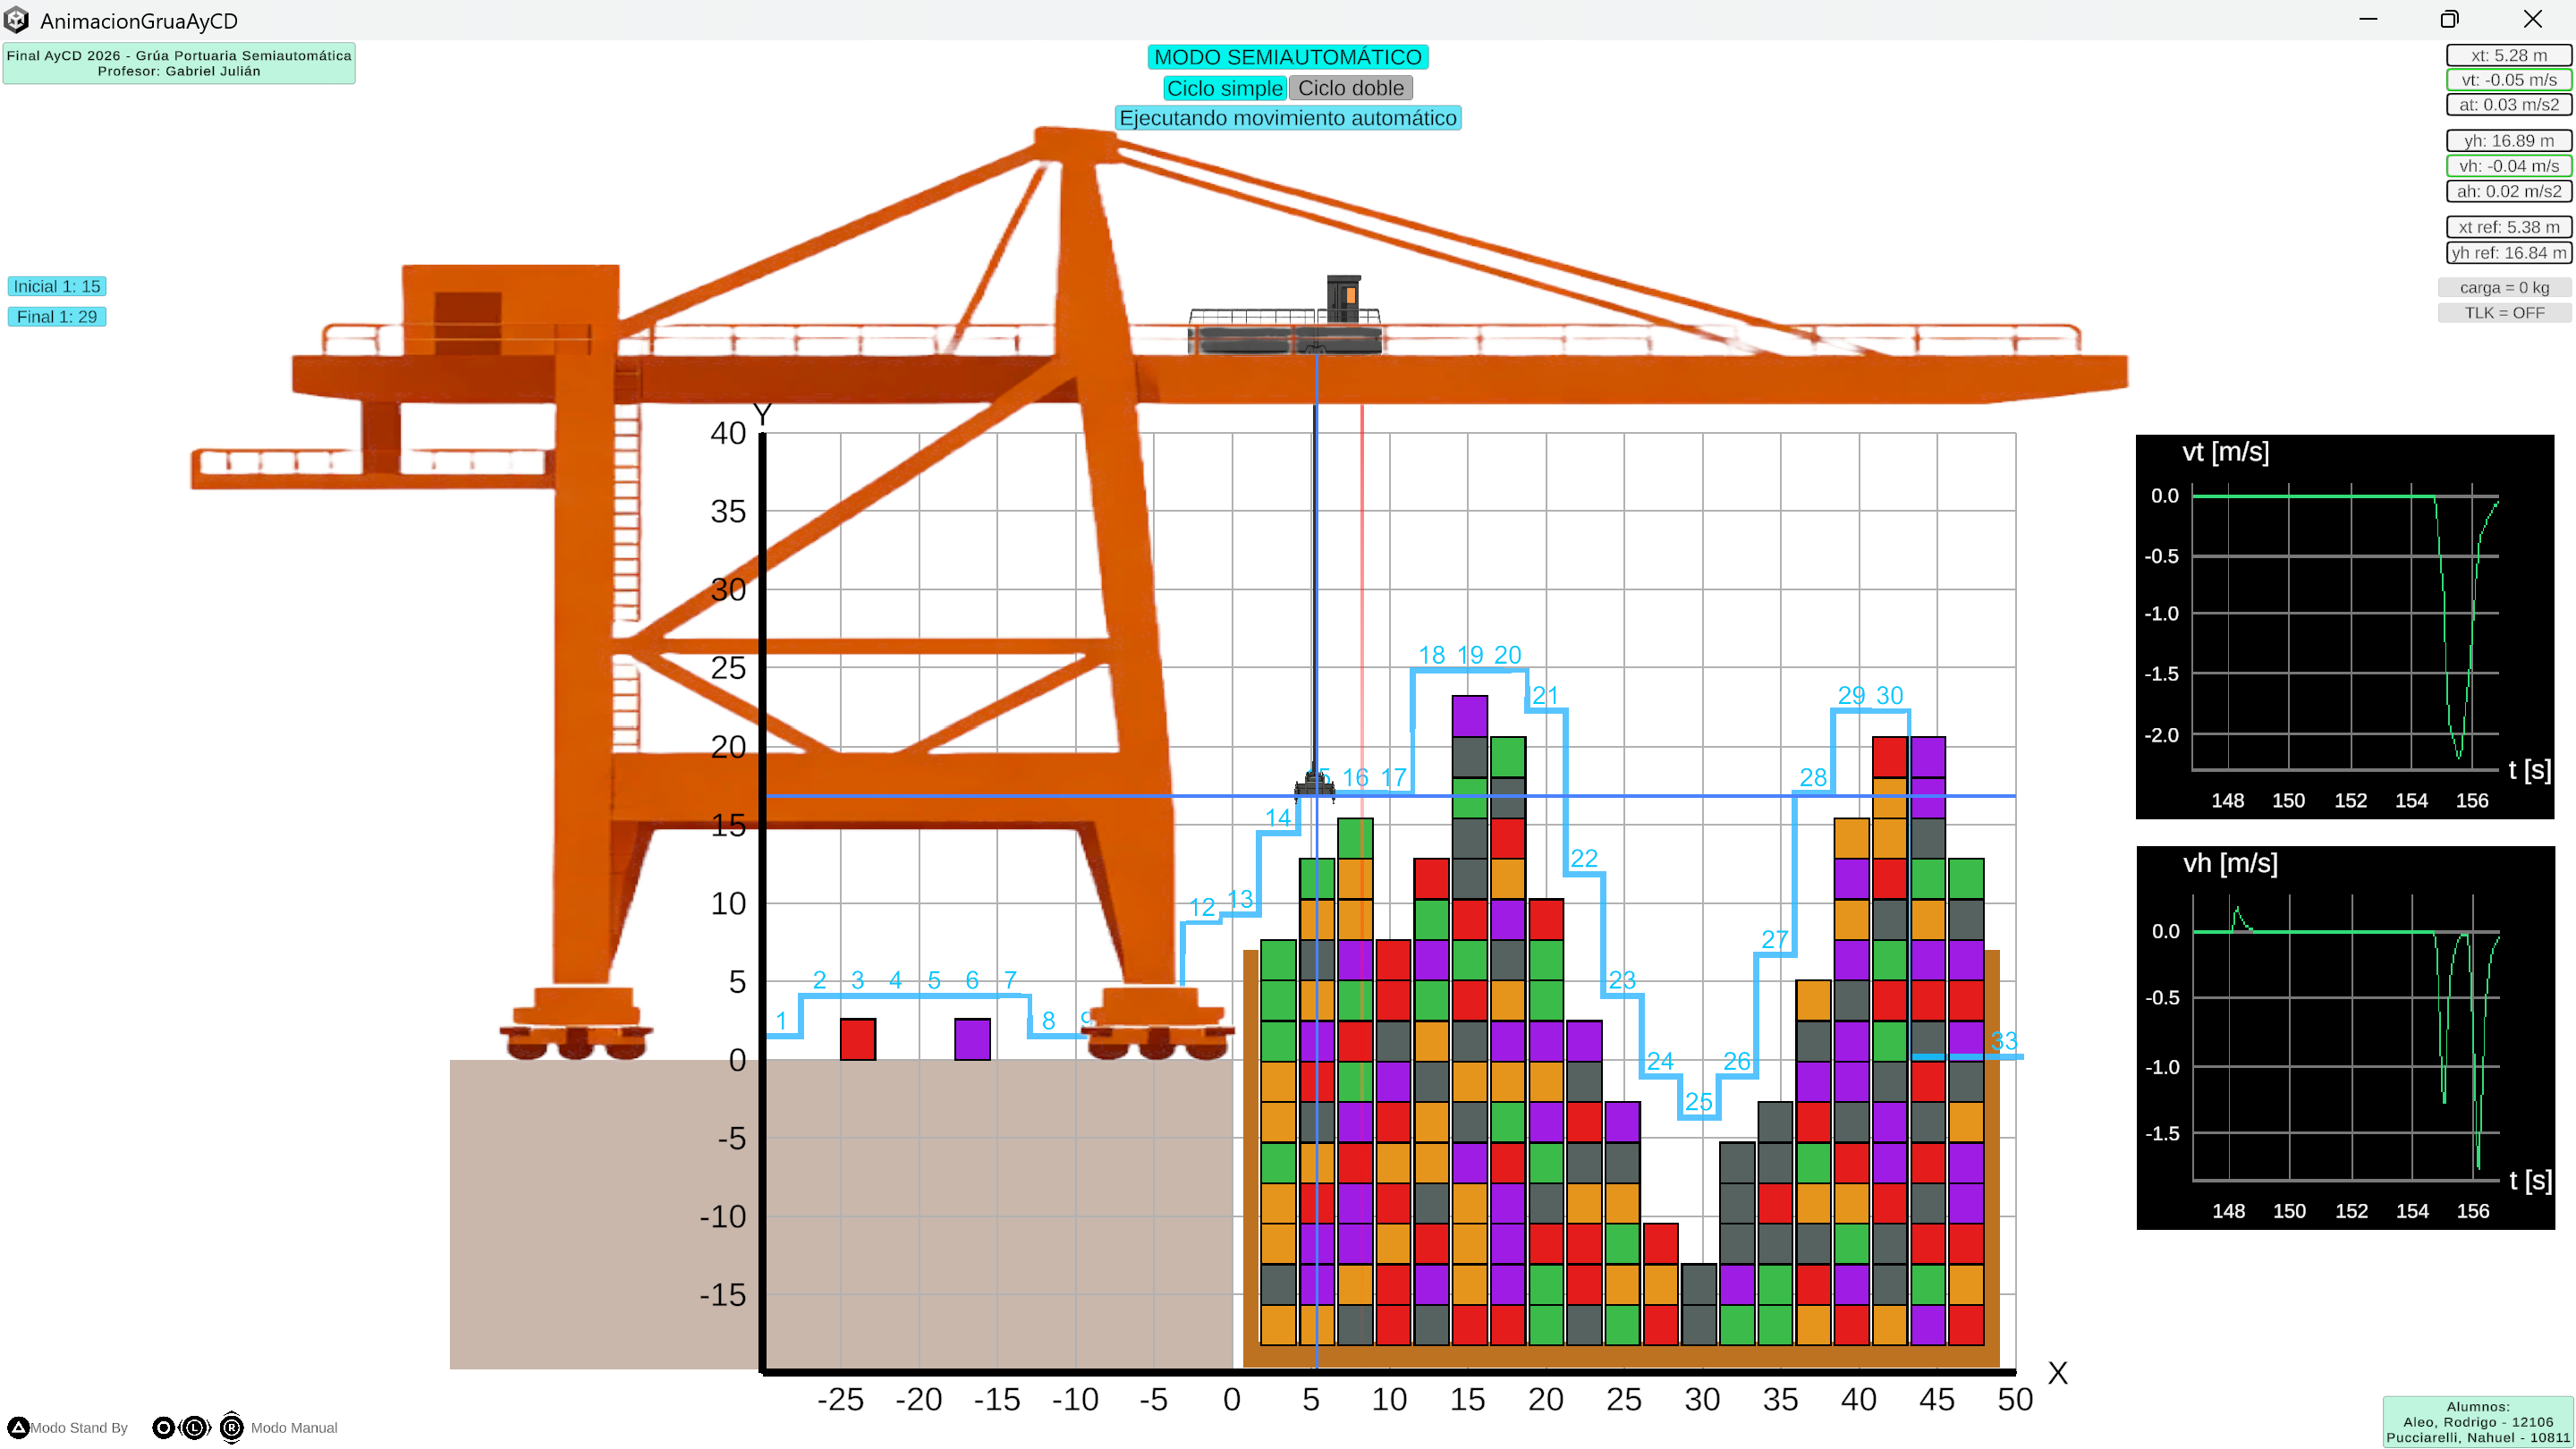
\includegraphics[width=1\textwidth]{unity_grua2.png}
    \caption{Modo Automático.}
\end{figure}
\begin{figure}[H]
    \centering
    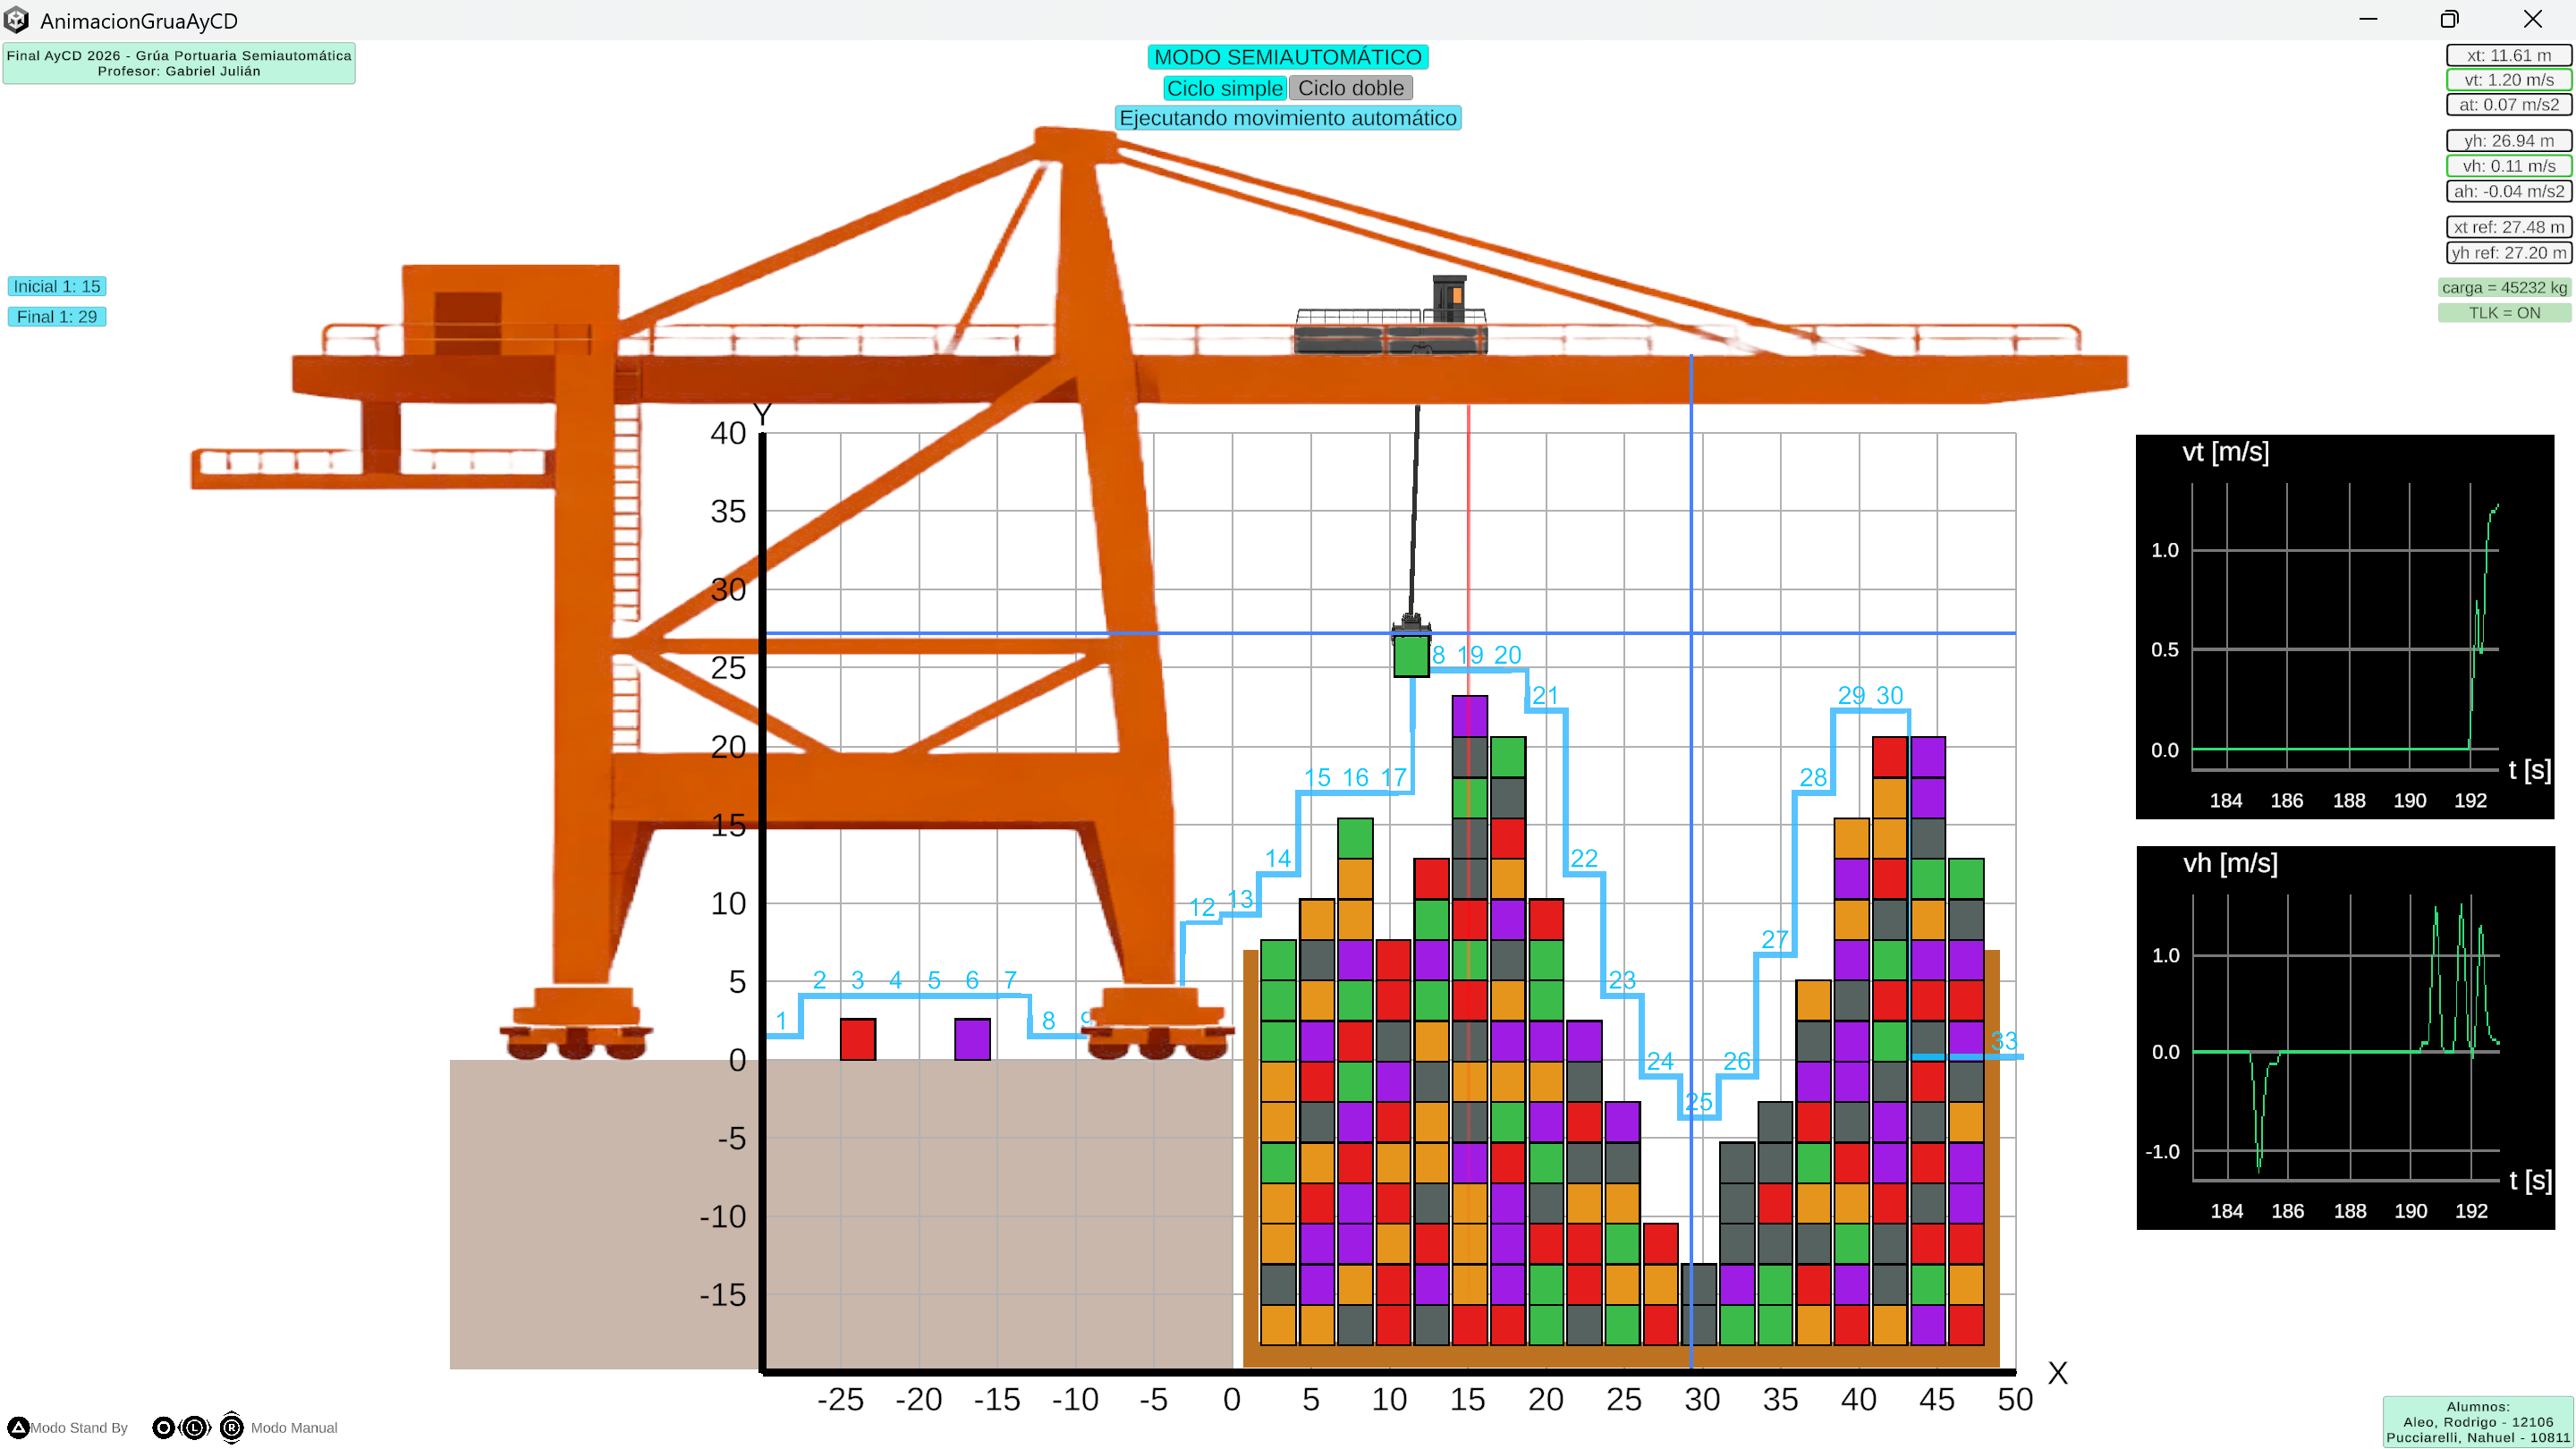
\includegraphics[width=1\textwidth]{unity_grua3.png}
    \caption{Modo Automático. Nótese la cruceta que muestra la posición objetivo a llevar el contenedor, con la masa ya estimada y la velocidad limitada según la curva de potencia.}
\end{figure}
\begin{figure}[H]
    \centering
    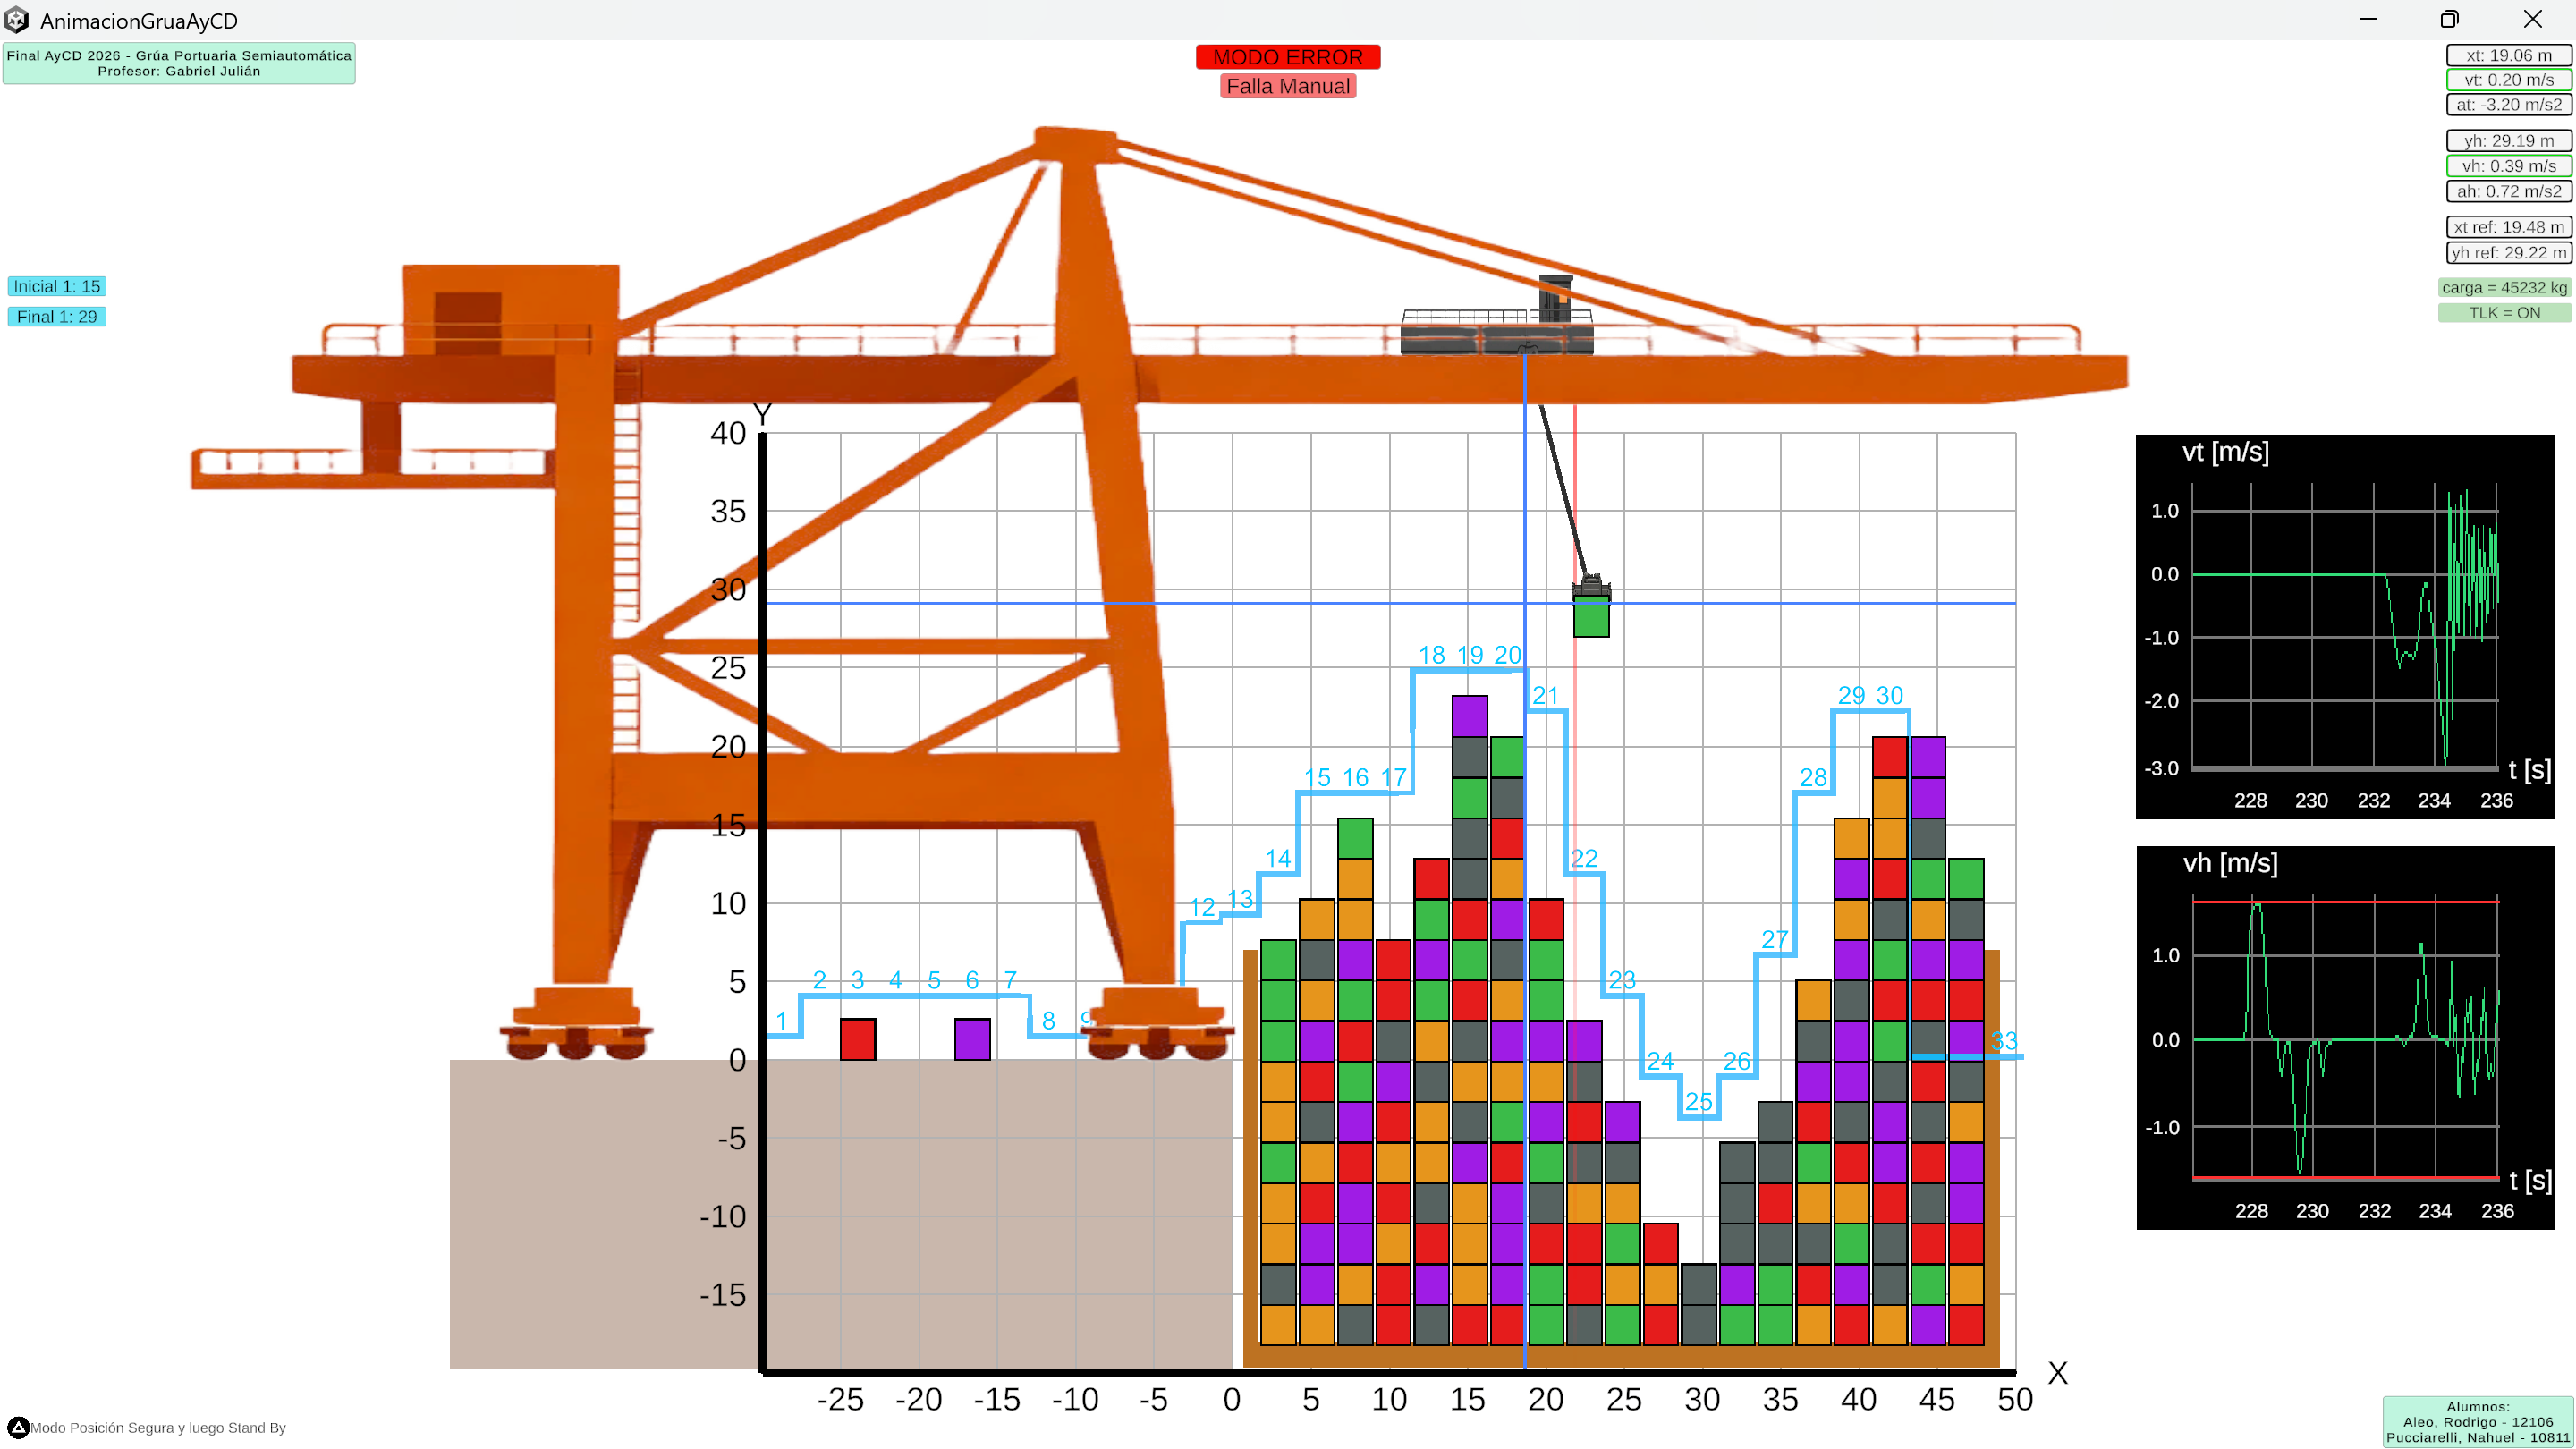
\includegraphics[width=1\textwidth]{unity_grua4.png}
    \caption{Modo Error Manual. Nótese que la grúa se detiene y se muestra un mensaje de error por haber apretado el botón de emergencia}
\end{figure}
\begin{figure}[H]
    \centering
    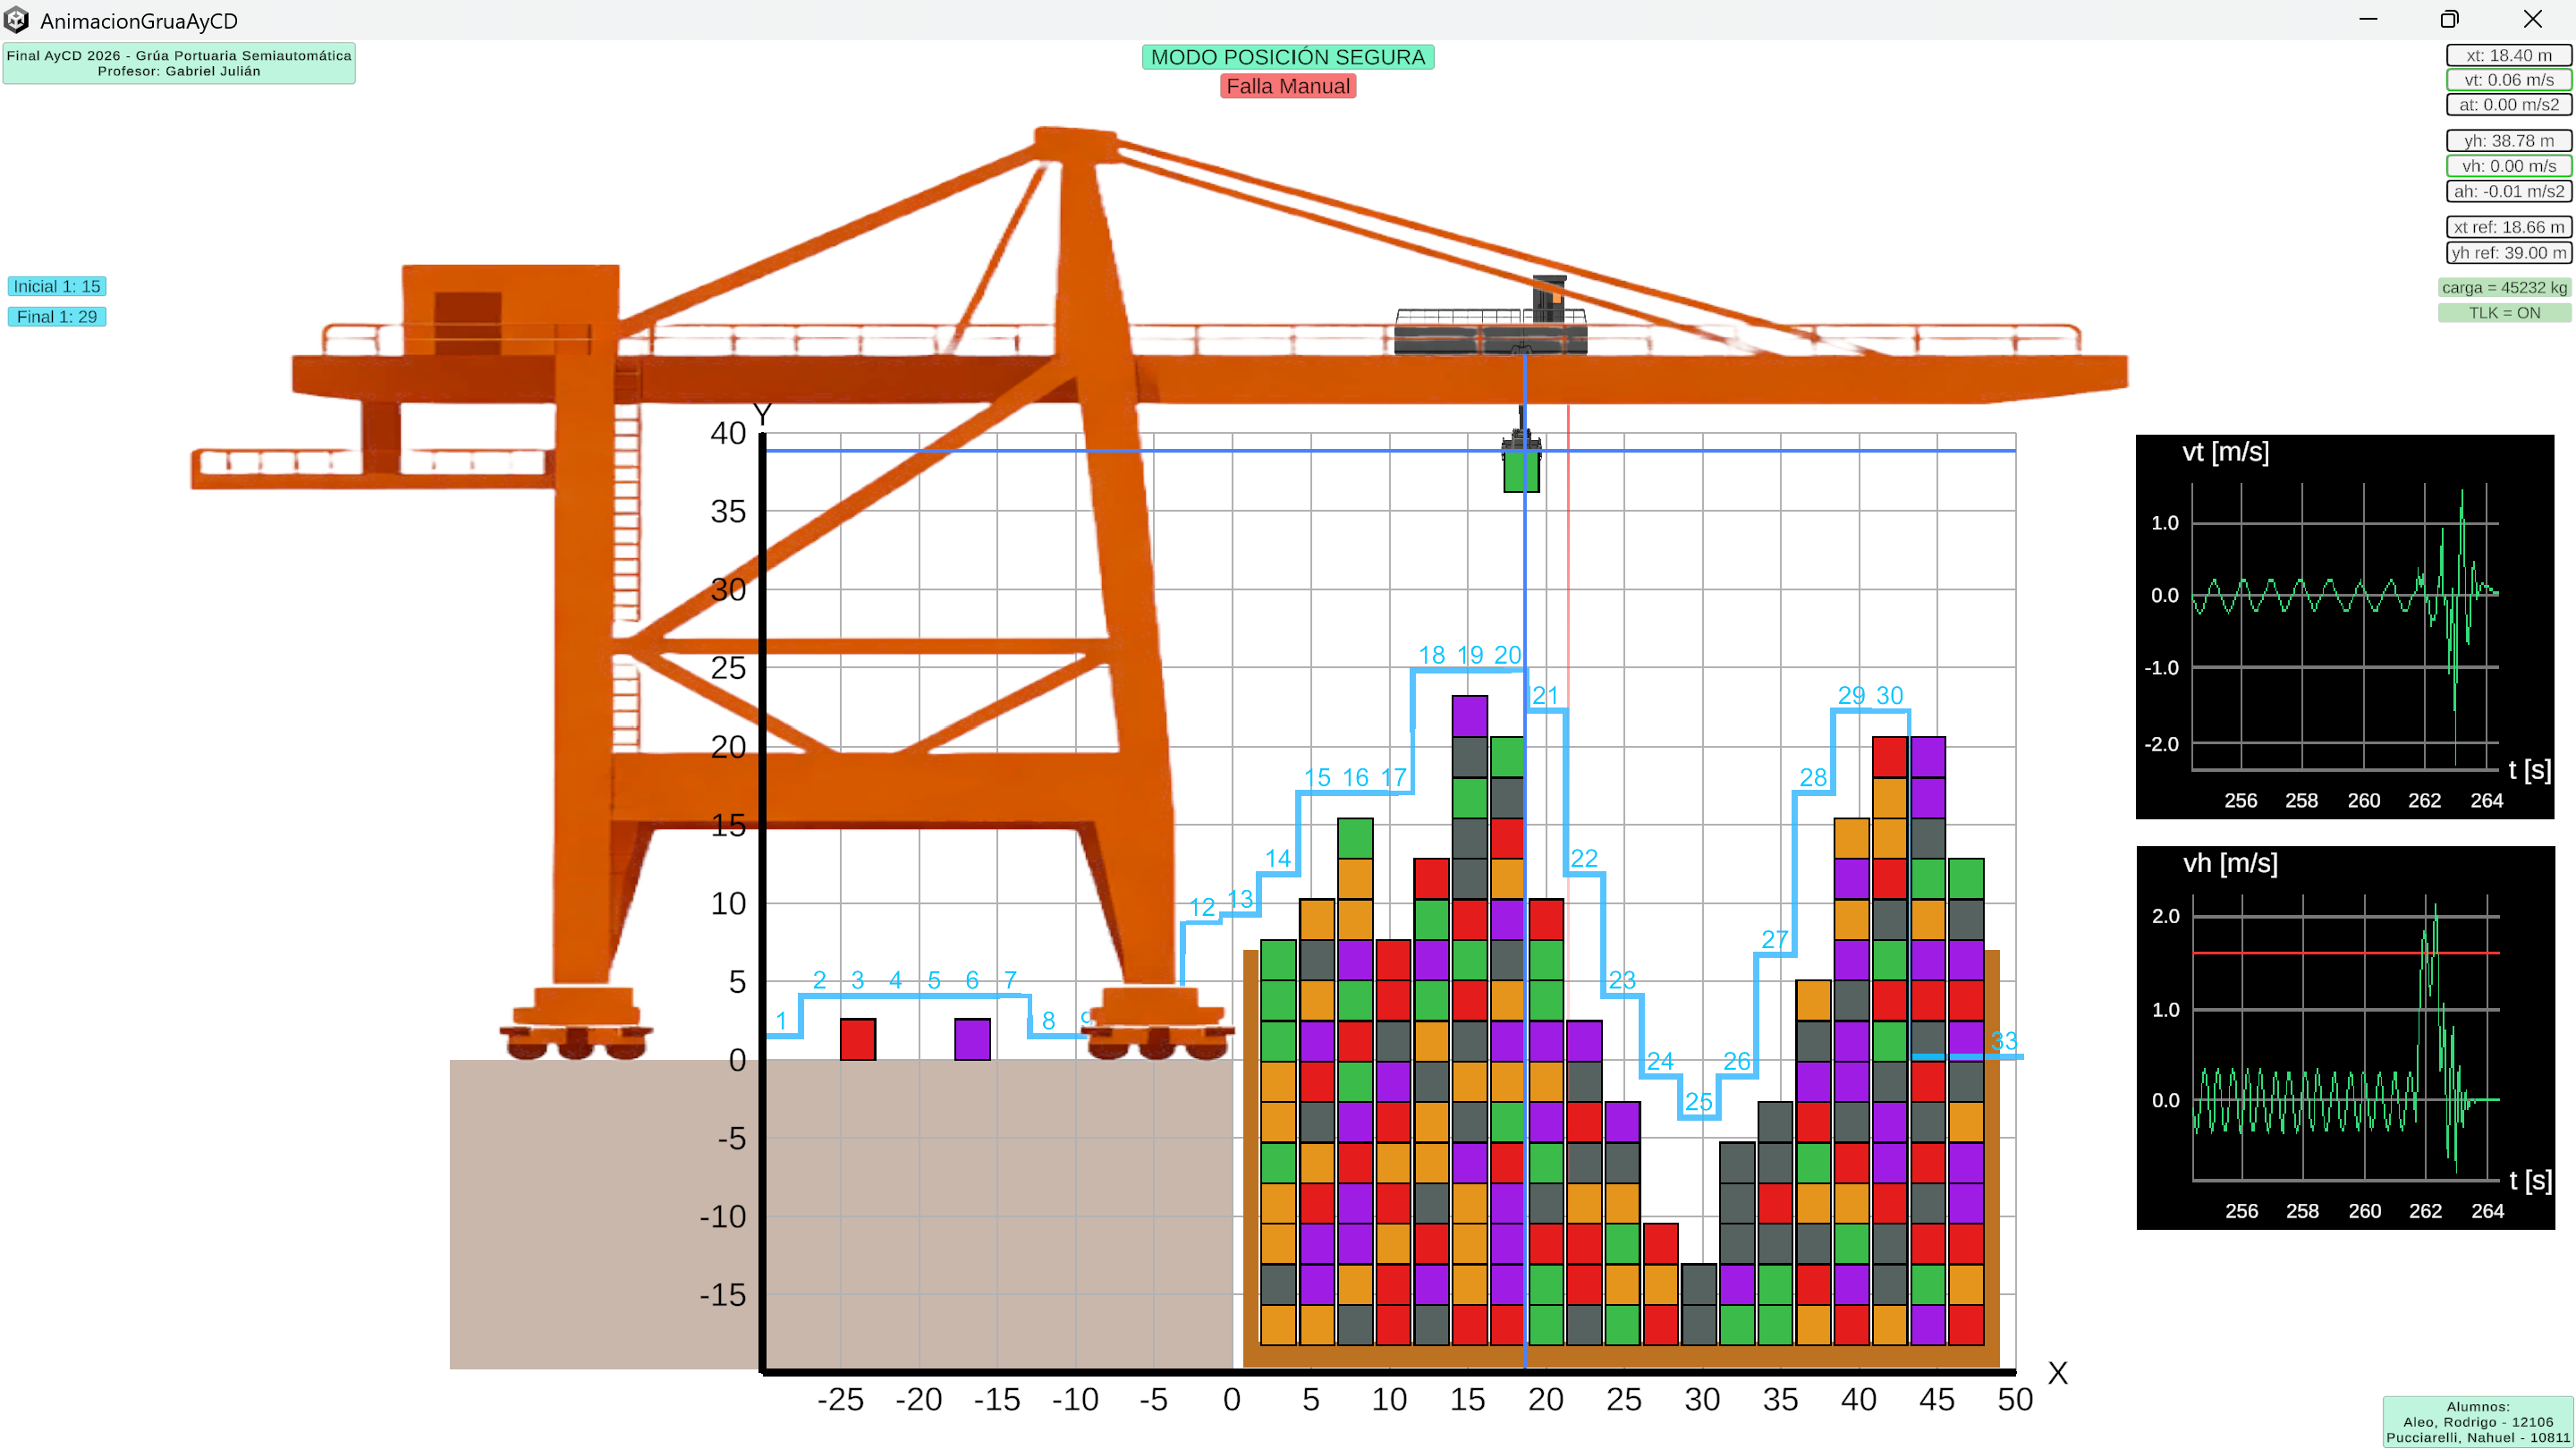
\includegraphics[width=1\textwidth]{unity_grua5.png}
    \caption{Modo de Posición Segura. De forma automática, la grúa se mueve a una posición de resguardo para proteger la integridad de la carga y el equipo.}
\end{figure}

\section{Diseño en ST y Codesys}
Todos los controladores se han diseñado en Stateflow, sin embargo, para la implementación en hardware real, se debe traducir la lógica desarrollada a un programa en Codesys utilizando el lenguaje de programación estructurado (ST). Este proceso implica mapear cada bloque funcional a funciones y estructuras de control equivalentes en ST, asegurando que la lógica de control se mantenga intacta durante la transición al entorno de ejecución real. Puede verse a continuación la estructura resultante:
\begin{figure}[H]
    \centering
    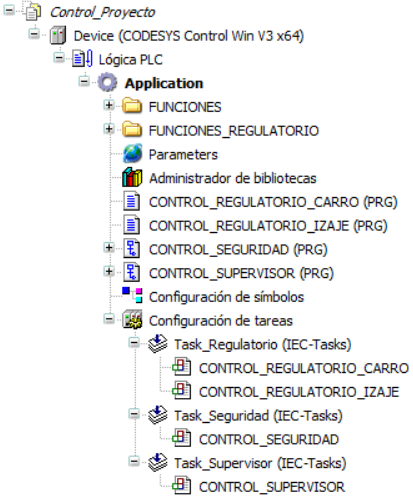
\includegraphics[width=0.5\textwidth]{arbol_codesys.png}
    \caption{Codesys - Árbol de componentes.}
\end{figure}

Los 4 POUs principales corresponden a los 3 niveles de control, separado el control regulatorio en control del carro y del izaje. Estos 4 programas se ejecutan de forma cíclica y en paralelo. Sin embargo en Codesys debido a la utilización de un PLC virtual con una sola CPU, estas tareas se ejecutan de forma secuencial pero de manera intercalada. A pesar de la limitación, se ejecuta a tal velocidad que, a fines prácticos, el comportamiento es idéntico al de un sistema con múltiples CPUs ejecutando tareas en paralelo (o múltiples PLCs).

\subsection{Control Regulatorio (Nivel 2) en Codesys}
Remitiéndose a la sección de diseño del control regulatorio, se rediseñó usando la misma lógica pero representándola con bloques de función de Matlab:
\begin{figure}[H]
    \centering
    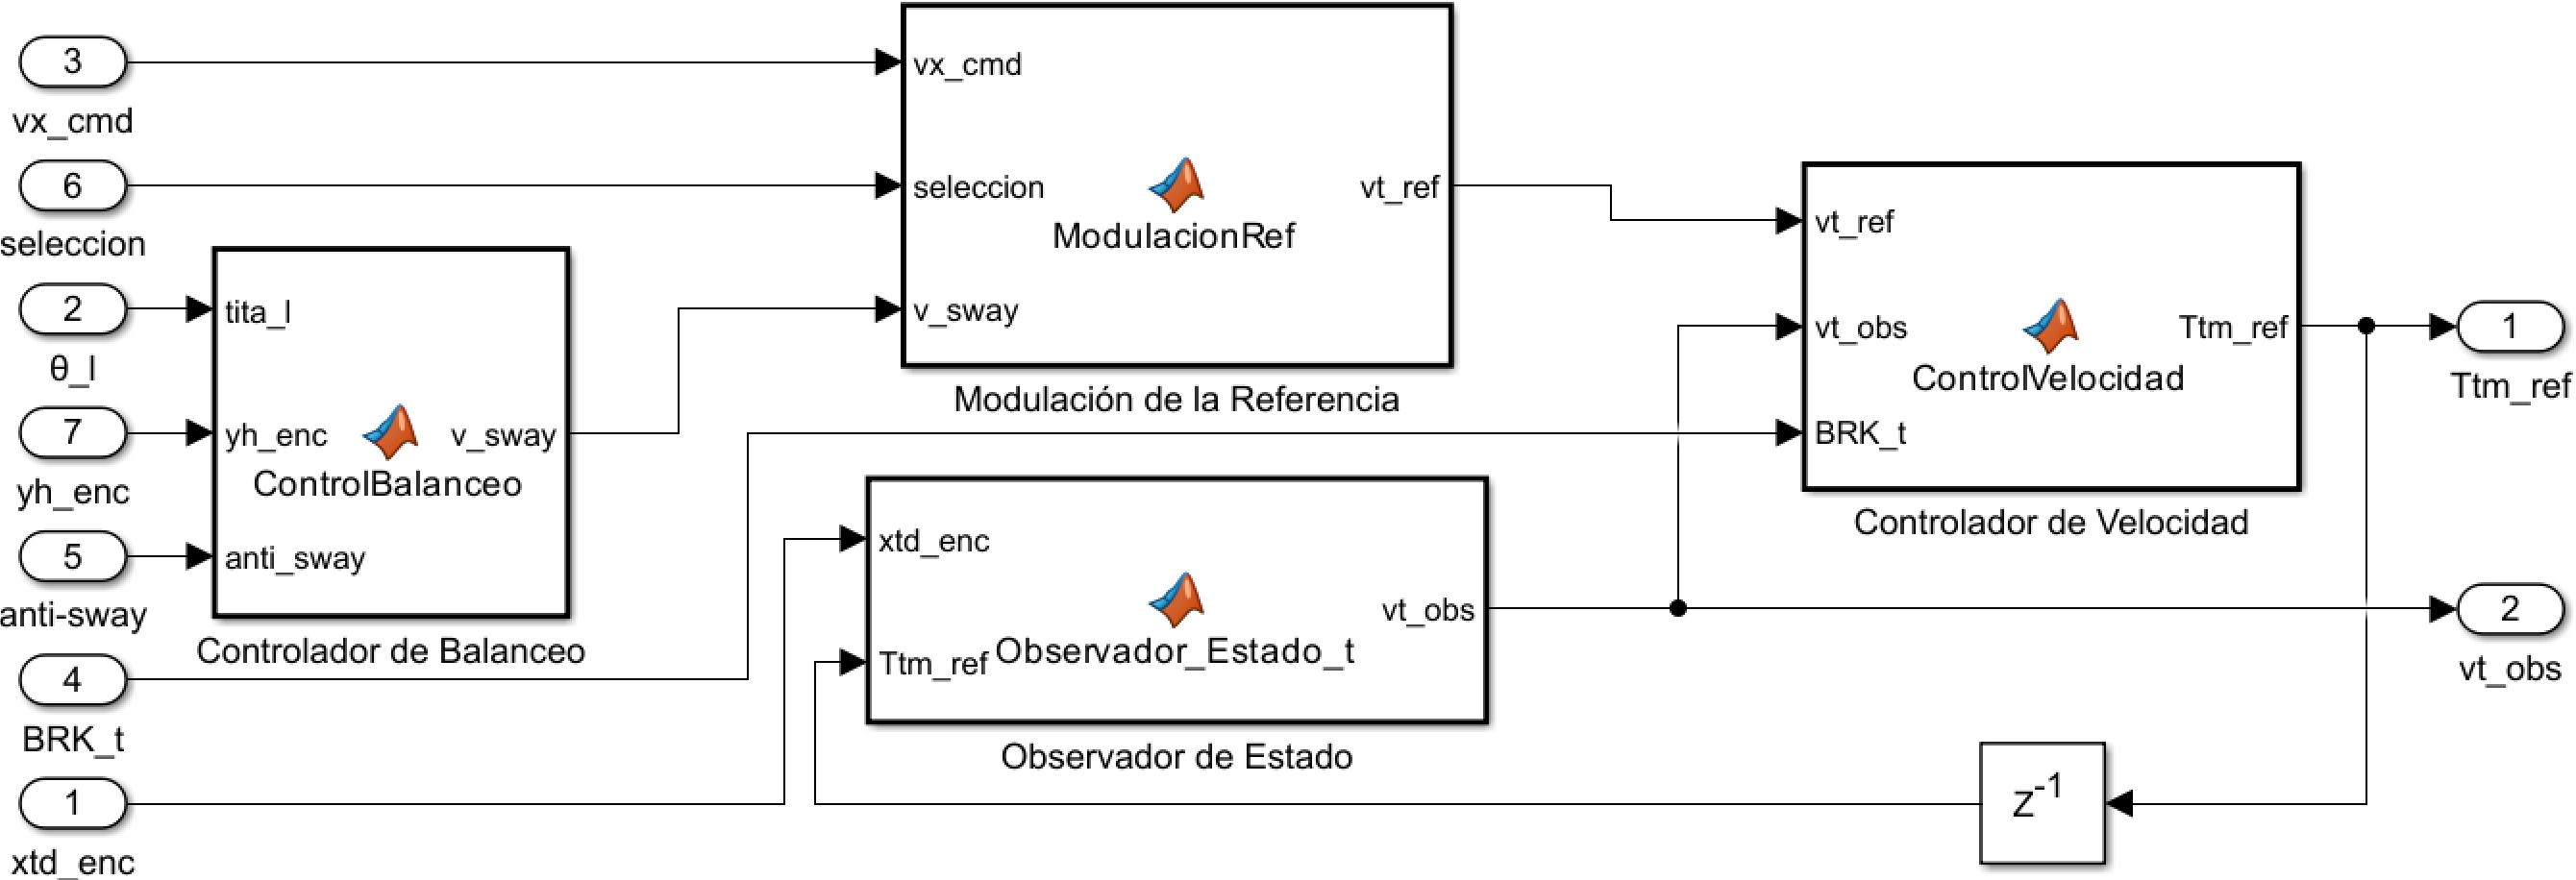
\includegraphics[width=1\textwidth]{control_carro_funciones2.png}
    \caption{Control del Carro con funciones de Matlab.}
\end{figure}
\begin{figure}[H]
    \centering
    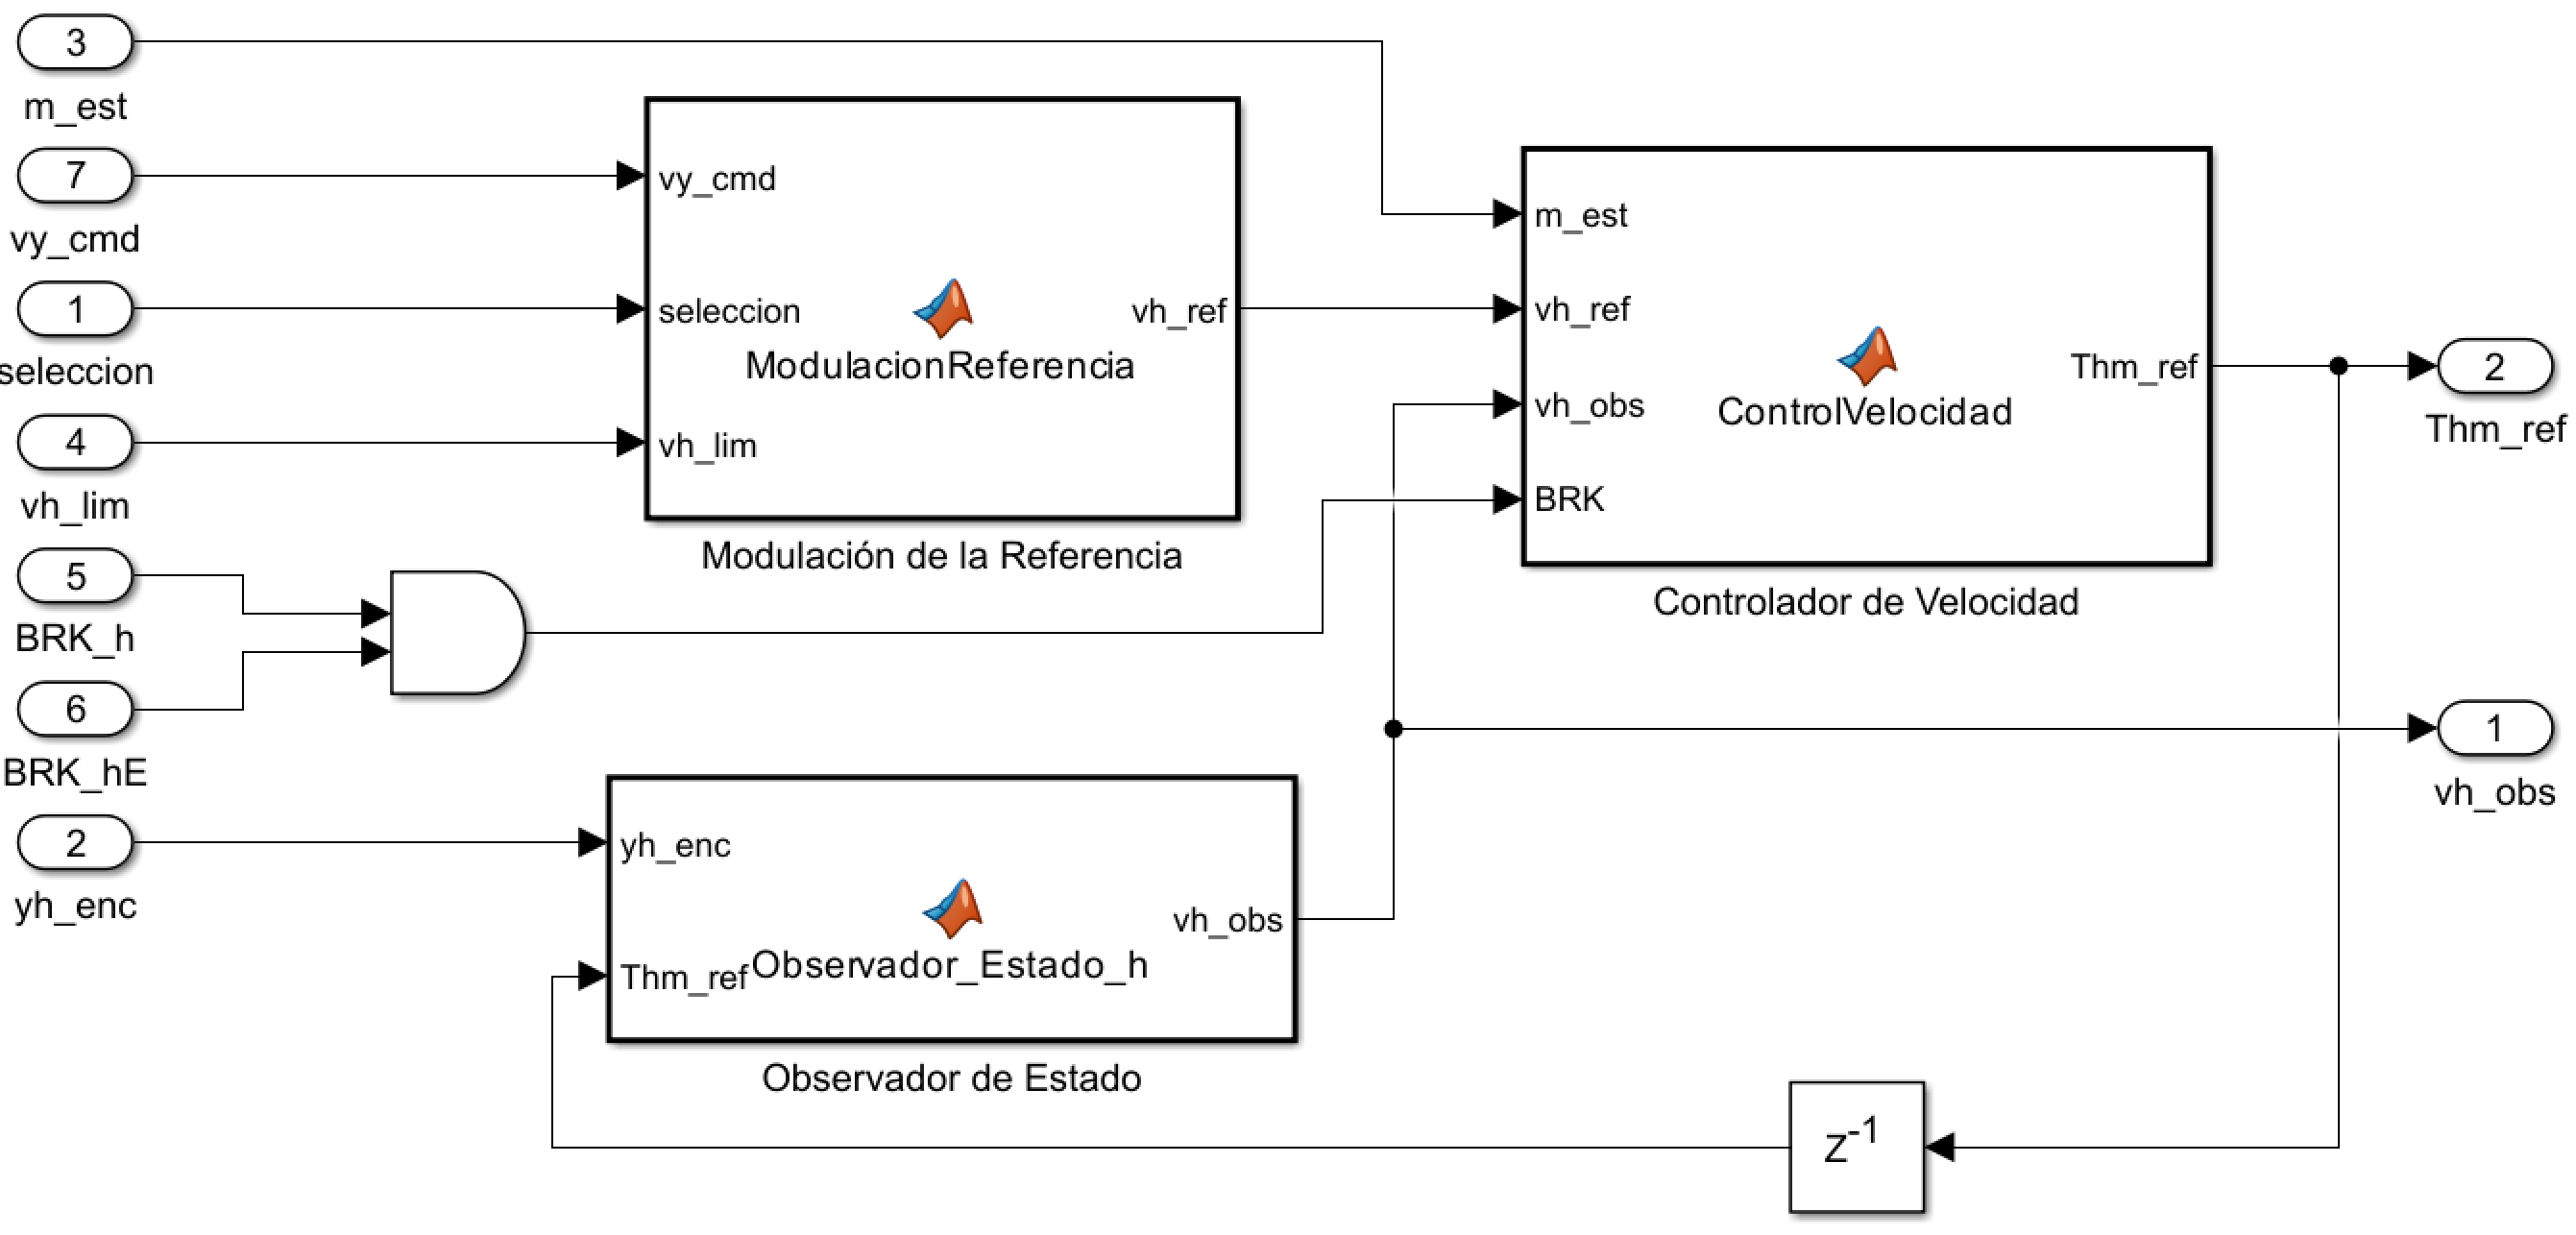
\includegraphics[width=1\textwidth]{control_izaje_funciones2.png}
    \caption{Control de Izaje con funciones de Matlab.}
\end{figure}

Una vez llevado a bloques de función es sencillo realizar la traducción a ST en Codesys, manteniendo la misma lógica de control.
\begin{figure}[H]
    \centering
    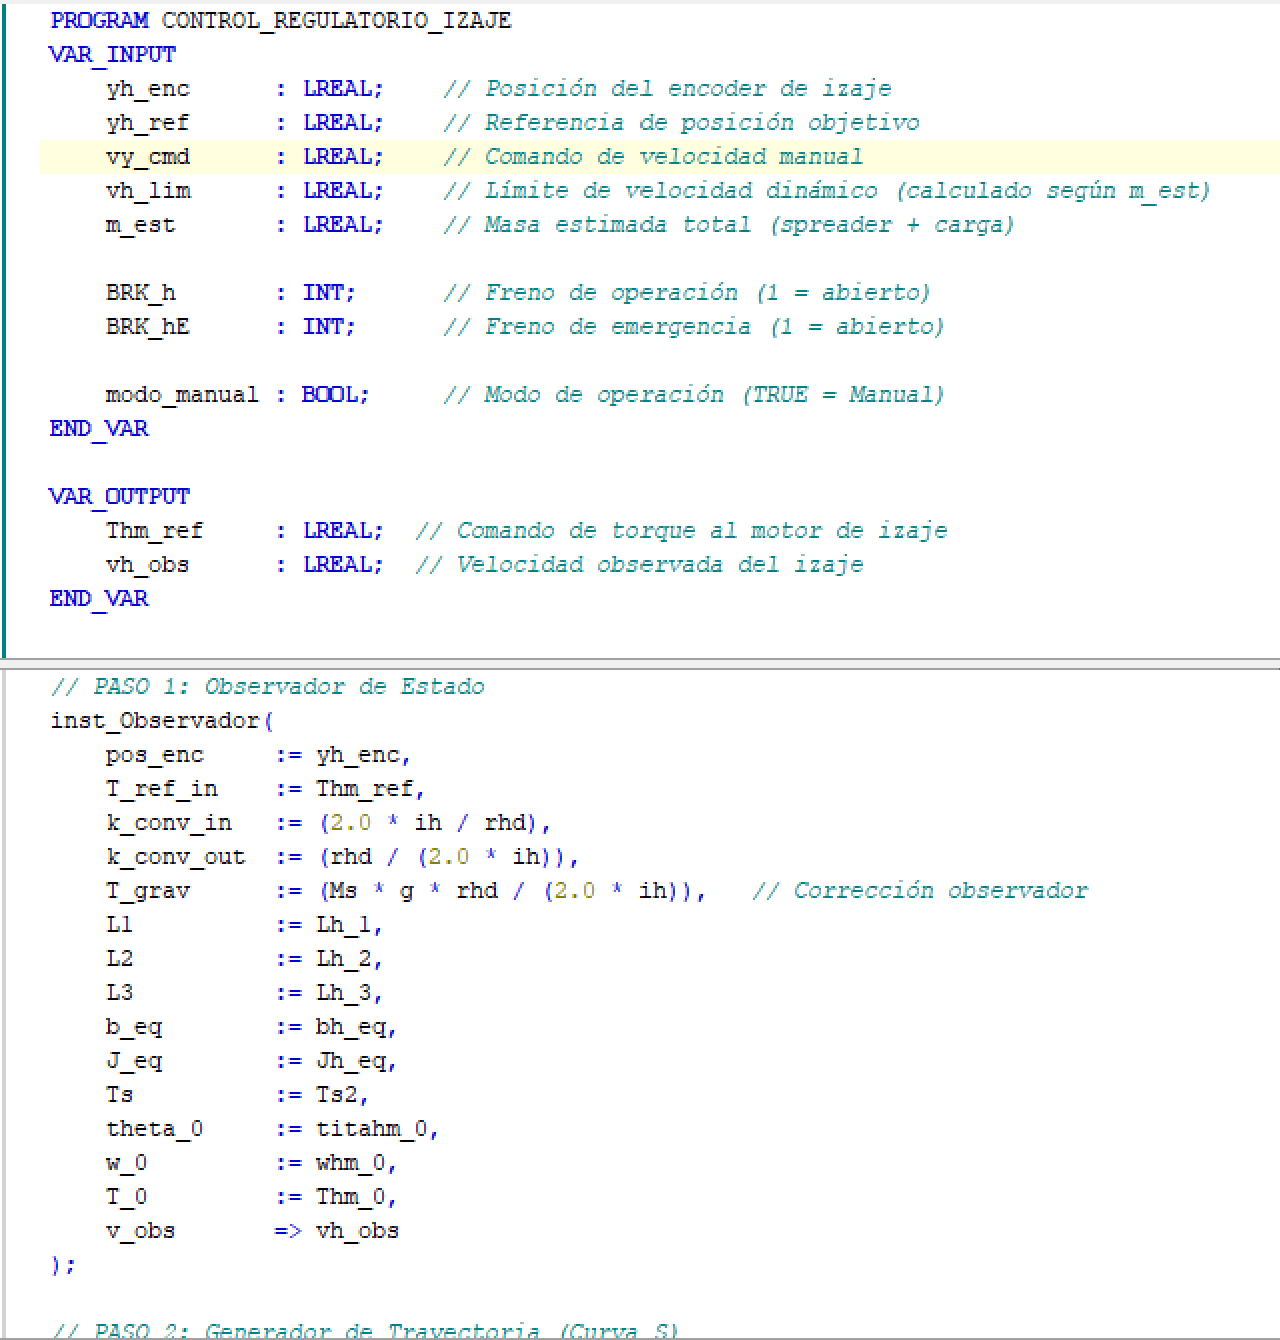
\includegraphics[width=0.8\textwidth]{codesys_regulatorio.png}
    \caption{Control de Izaje en Codesys (ST).}
\end{figure}

\subsection{Control Supervisor (Nivel 1) en Codesys}
Para el control supervisor se debe repensar la forma de traducir los bloques de Stateflow a SFC, ya que no es tan directo. De este proceso se obtuvo un conjunto de varios bloques en paralelo:
\begin{figure}[H]
    \centering
    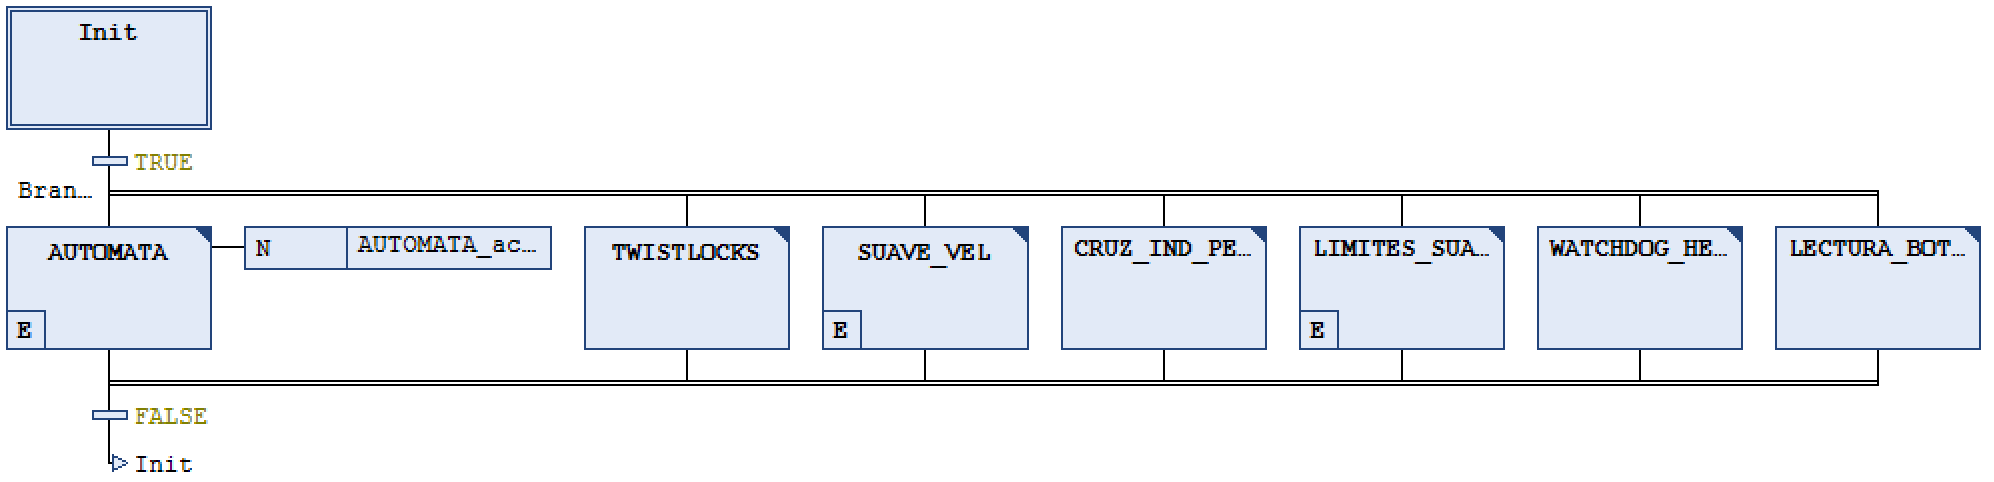
\includegraphics[width=1\textwidth]{codesys_supervisor11.png}
    \caption{Codesys - Diagrama general de control supervisor.}
\end{figure}
A diferencia de Stateflow, se debe agregar un estado paralelo adicional \texttt{LECTURA\_BOTONES}, el cuál se encarga exclusivamente de detectar flancos de subida de los botones presionados por el usuario.

El autómata principal se desarrolla de forma similar, y se encarga de alternar entre los modos de Stand By, Manual, Automático, Errores y Recuperación. 
\begin{figure}[H]
    \centering
    \begin{subfigure}{1\textwidth}
        \centering
        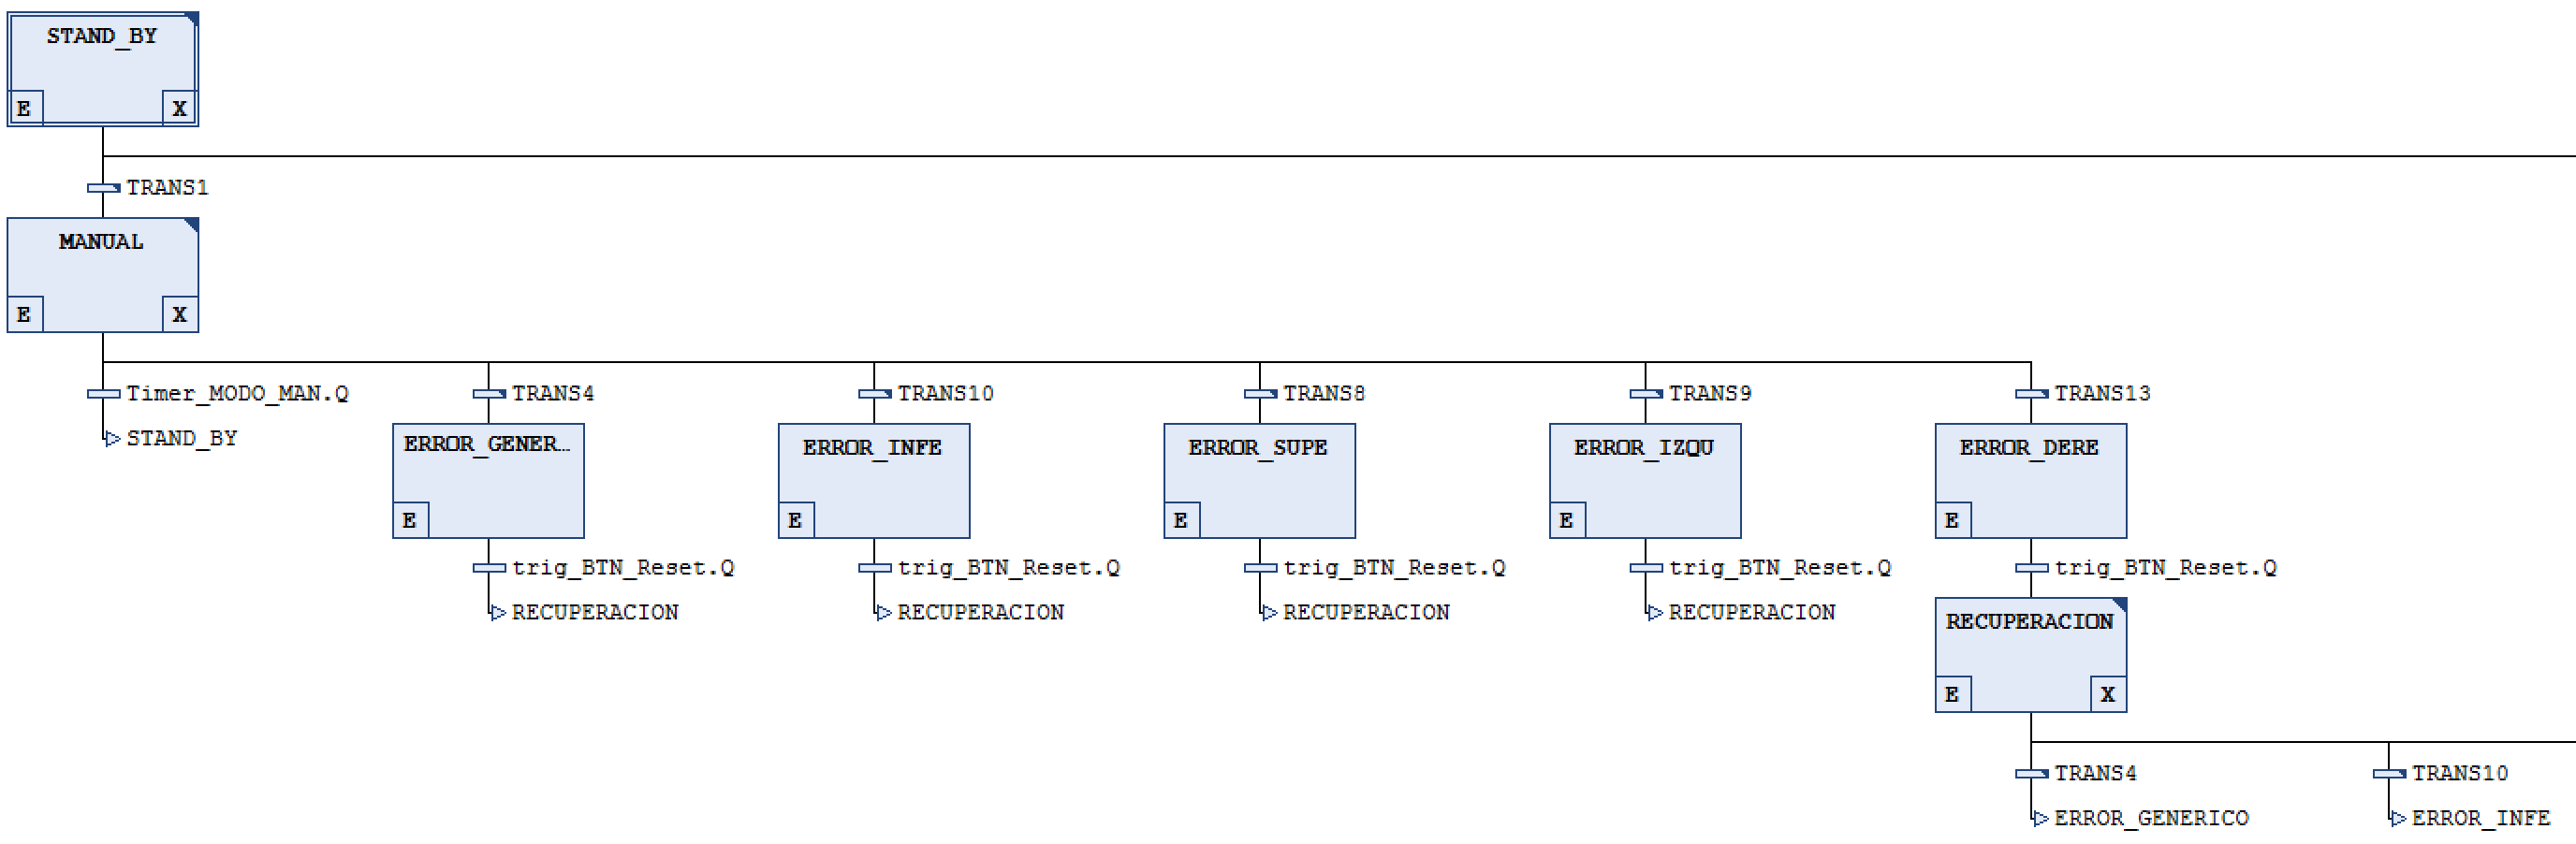
\includegraphics[width=\linewidth]{codesys_supervisor12.png}
    \end{subfigure}
    \begin{subfigure}{1\textwidth}
        \centering
        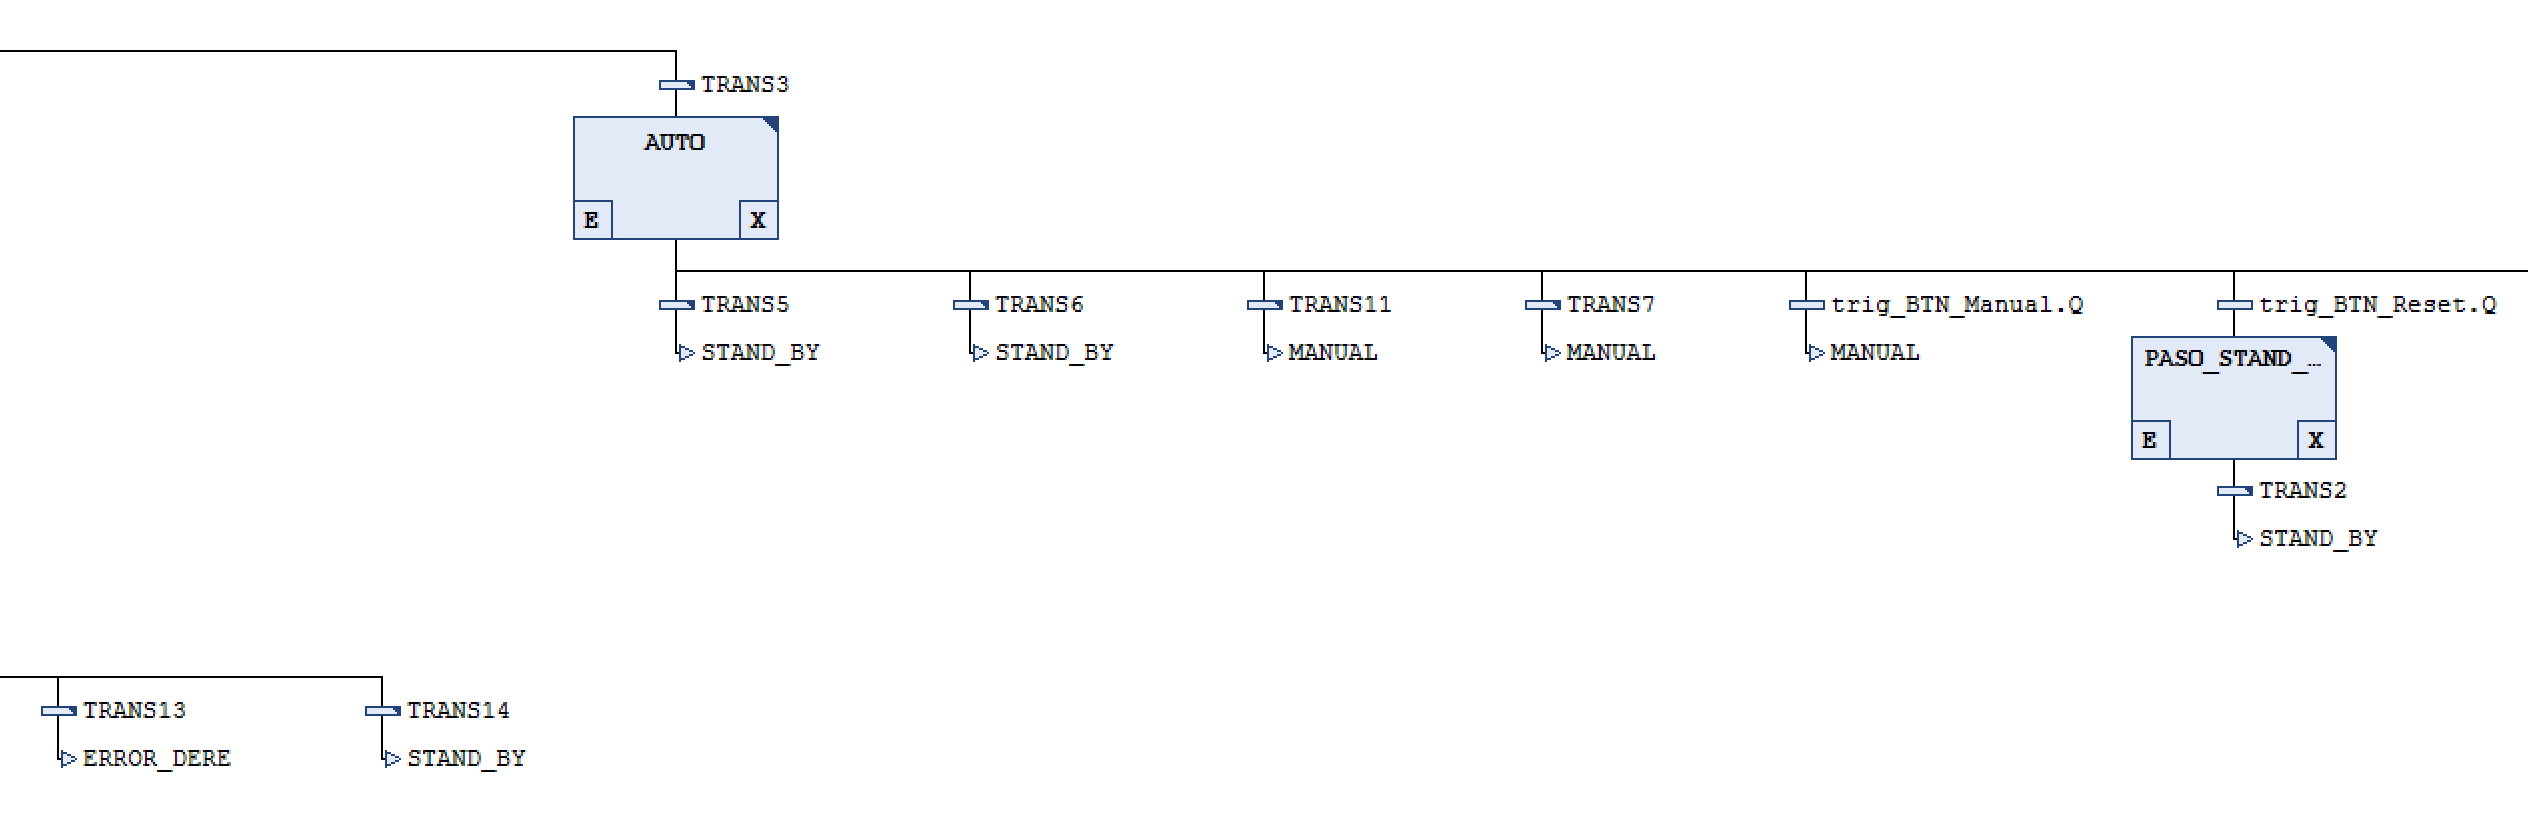
\includegraphics[width=\linewidth]{codesys_supervisor13.png}
    \end{subfigure}
    \caption{Codesys - Supervisor - Autómata principal.}
\end{figure}

Para el modo automático se tuvo que modificar ligeramente las transiciones. En SFC, si se interrumpe un paso y salimos del modo automático, al volver al mismo no comienza por el paso inicial, sino que retoma en el paso interrumpido. Para evitar este comportamiento indeseado se agregó una variable adicional que permite transicionar al paso inicial. Esto no ocurre en Stateflow, ya que al entrar el modo automático éste siempre comienza a ejecutarse desde el estado inicial. En la siguiente imágen se puede ver la implementación utilizada:
\begin{figure}[H]
    \centering
    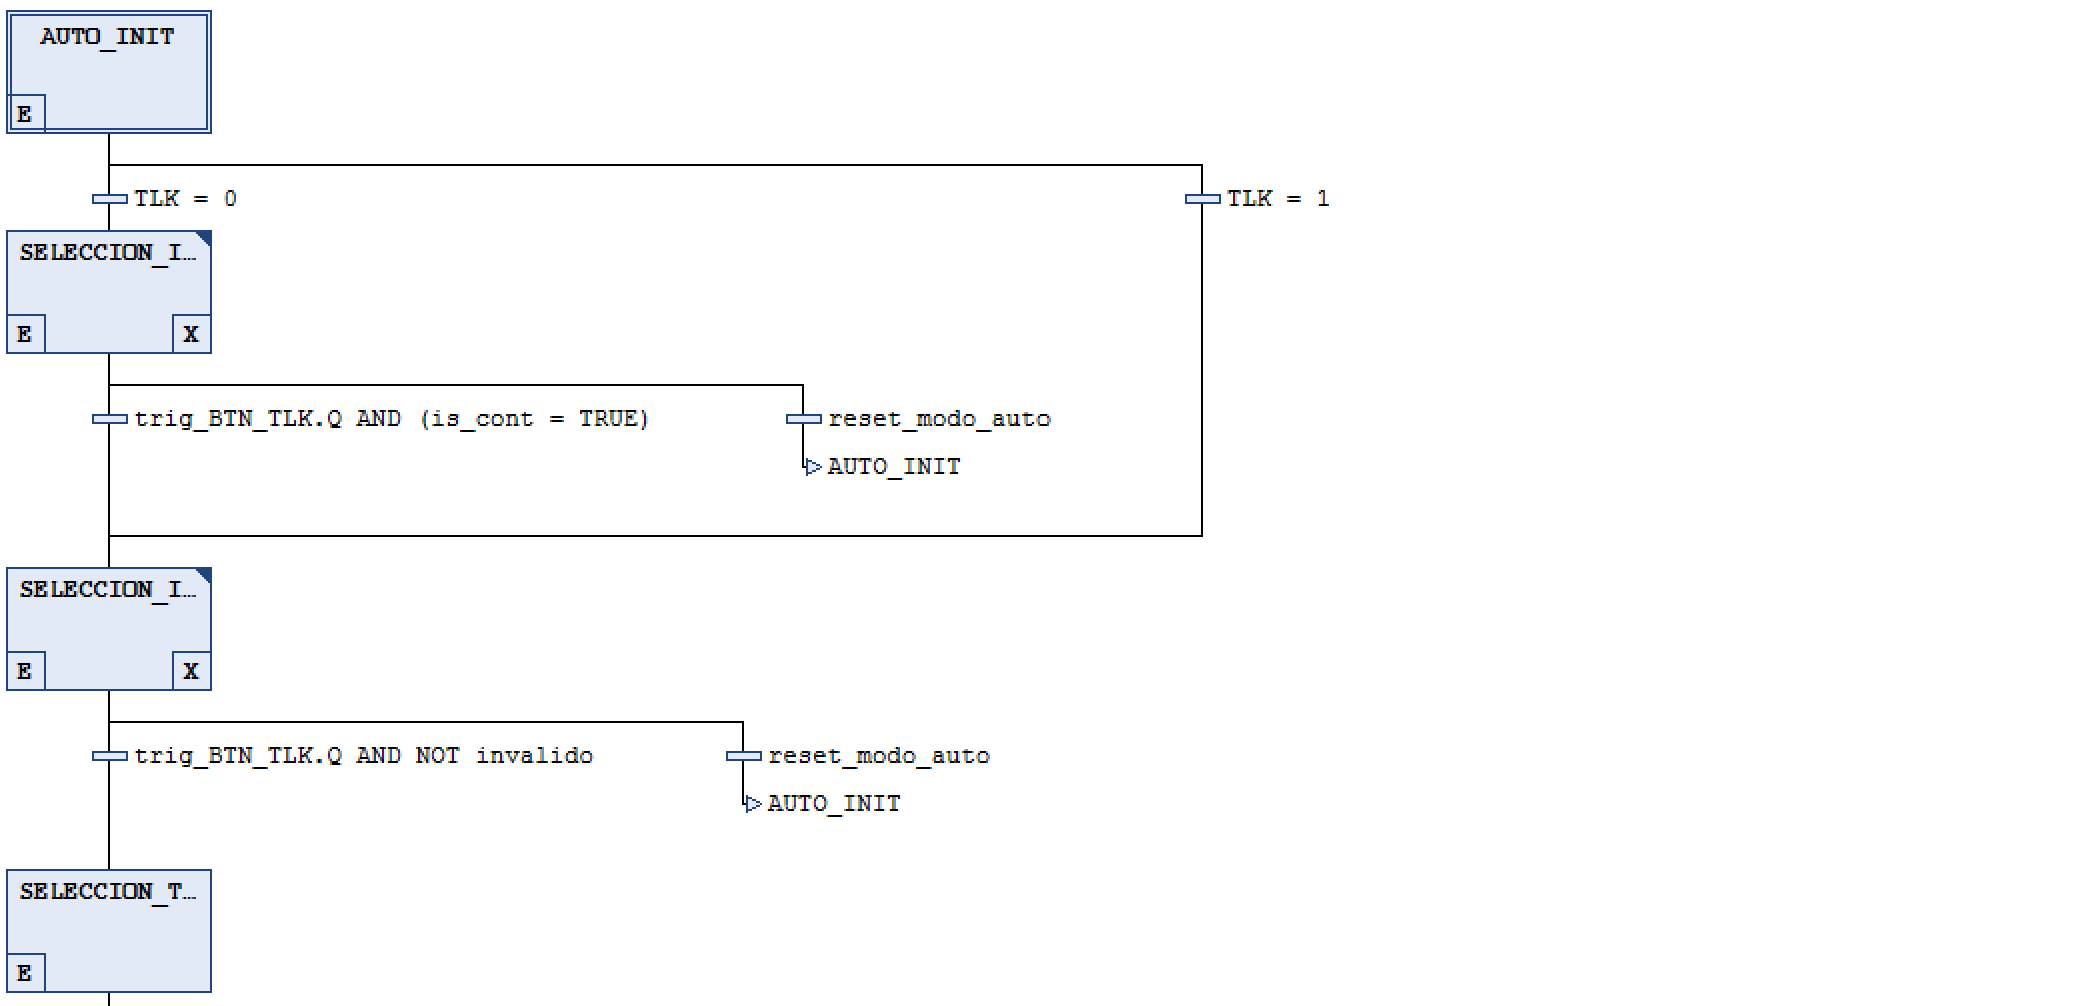
\includegraphics[width=1\textwidth]{codesys_supervisor15.png}
\end{figure}
\begin{figure}[H]
    \centering
    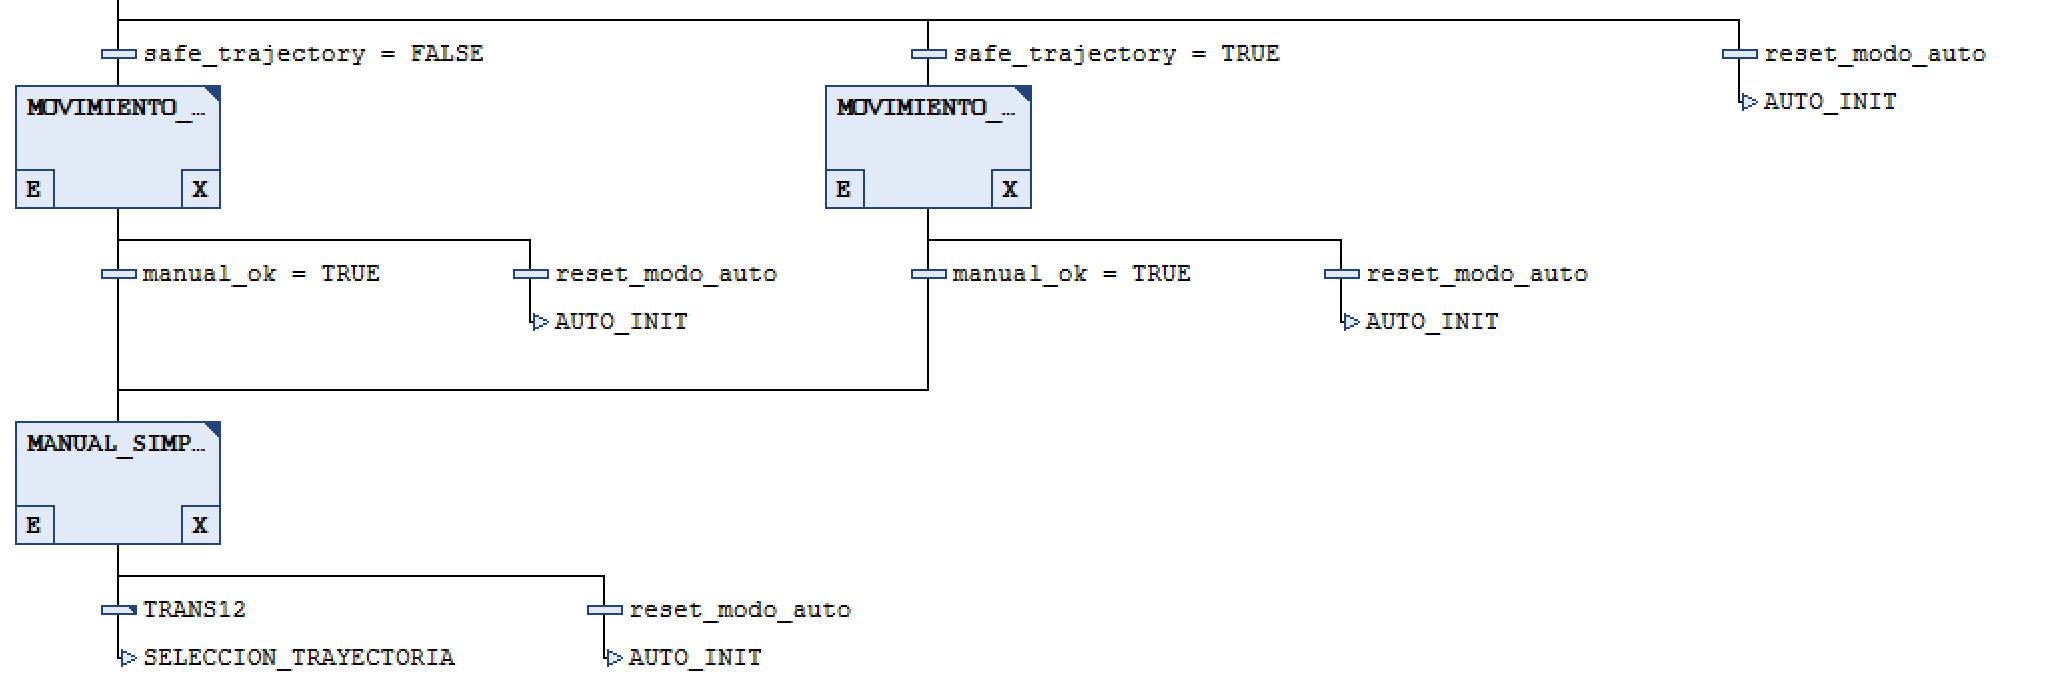
\includegraphics[width=1\textwidth]{codesys_supervisor16.png}
    \caption{Codesys - Supervisor - Autómata principal - Auto.}
\end{figure}

Sin modificaciones notorias, se replica el bloque encargado de la lógica de los Twistlocks. Como es un SFC cíclico, el último paso regresa al inicial al cumplir su transición:
\begin{figure}[H]
    \centering
    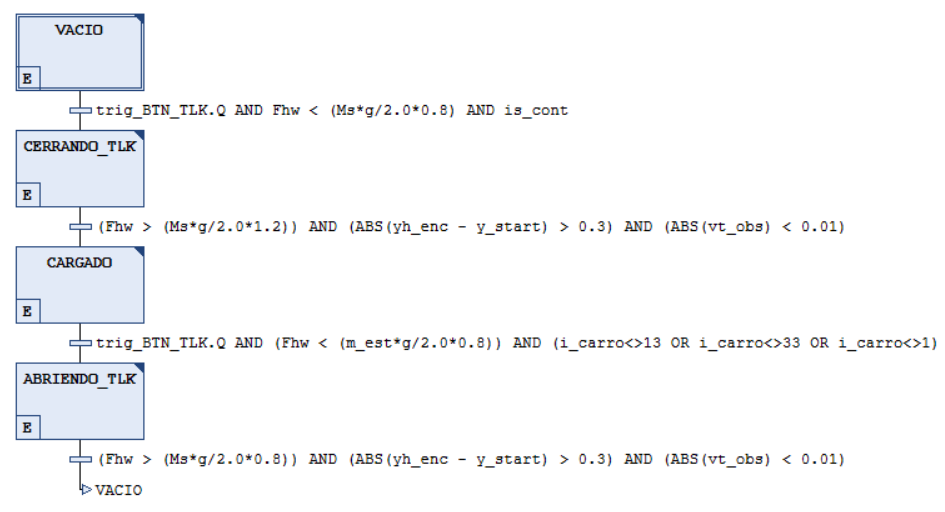
\includegraphics[width=1\textwidth]{codesys_supervisor4.png}
    \caption{Codesys - Supervisor - Lógica de Twistlocks.}
\end{figure}

De la misma forma, se utilizan las entradas de los sensores para calcular la posición discreta del carro y actualizar el perfil de obstáculos, información que es fundamental para la generación de trayectorias seguras en modo automático. También se actualiza la posición de la cruceta:
\begin{figure}[H]
    \centering
    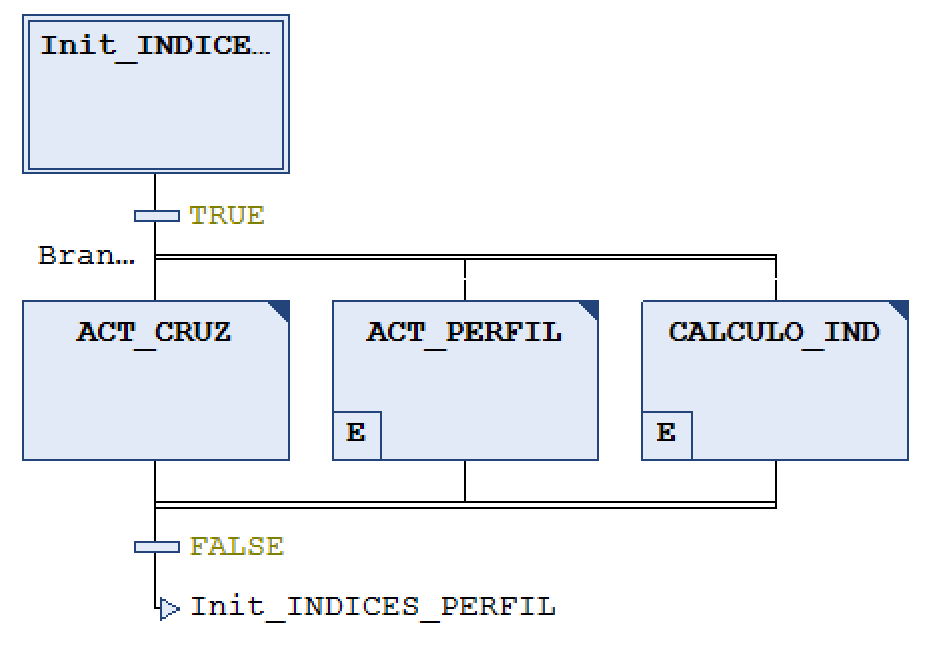
\includegraphics[width=0.55\textwidth]{codesys_supervisor14.png}
    \caption{Codesys - Supervisor - Cruceta Índices Perfil.}
\end{figure}

Los bloques de \textit{Suavizador Velocidad}, \textit{Límites Suave} y \textit{Watchdog Heartbeat} se mantienen prácticamente iguales, desarrollados en ST directamente debido a su sencillez.

\subsection{Control de Seguridad (Nivel 0) en Codesys}
Para el control de seguridad se mantuvo el mismo diseño, esta vez con dos procesos paralelos, uno para la máquina de estados de seguridad y otro para el watchdog. La lógica de ambos procesos se mantuvo prácticamente igual, con pequeñas modificaciones para adaptarse a la sintaxis y estructura de SFC.
\begin{figure}[H]
    \centering
    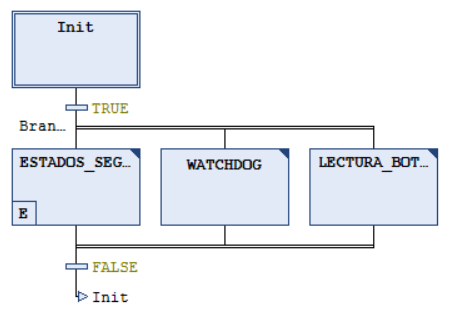
\includegraphics[width=0.5\textwidth]{codesys_seguridad1.png}
    \caption{Codesys - Seguridad - Diagrama general del control de seguridad.}
\end{figure}

\begin{figure}[H]
    \centering
    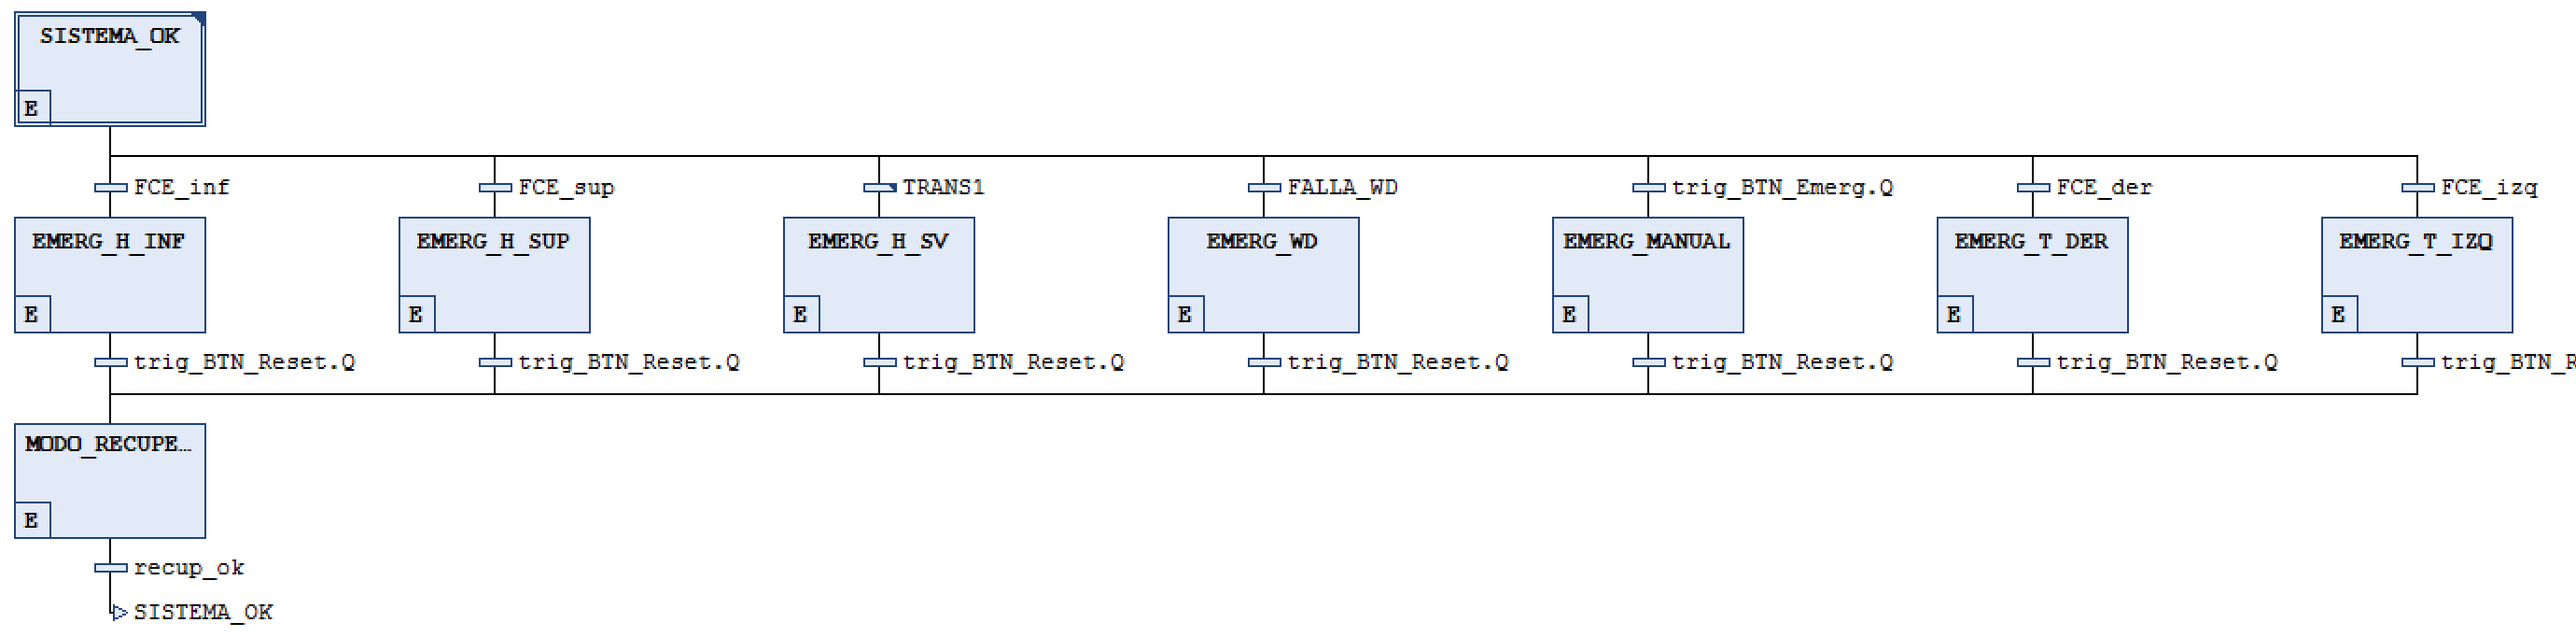
\includegraphics[width=1\textwidth]{codesys_seguridad22.png}
    \caption{Codesys - Seguridad - Estados de Seguridad.}
\end{figure}

\begin{figure}[H]
    \centering
    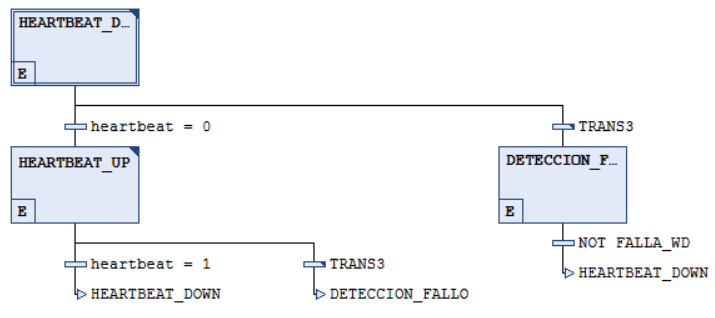
\includegraphics[width=0.8\textwidth]{codesys_seguridad3.png}
    \caption{Codesys - Seguridad - Watchdog.}
\end{figure}

\subsection{Comunicación Simulink-Codesys}
Para poder comunicar el PLC virtual de Codesys con Simulink, se utilizó el protocolo de comunicación industrial \texttt{OPC-UA}. La versión de Codesys utilizada (CODESYS V3.5 SP21 Patch 2) cuenta con la posibilidad de montar un servidor OPC-UA y de seleccionar qué variables del programa se quieren exponer a través de este protocolo. Por otro lado, Matlab R2025b cuenta con un cliente OPC-UA que permite conectarse a este servidor y leer/escribir las variables expuestas en tiempo real.

Para permitir una conexión adecuada, se modificó algunos ajustes del dispositivo que hace de servidor. Se configuró sin encriptación, y la configuración de Device Security Settings se ve de la siguiente forma:
\begin{figure}[H]
    \centering
    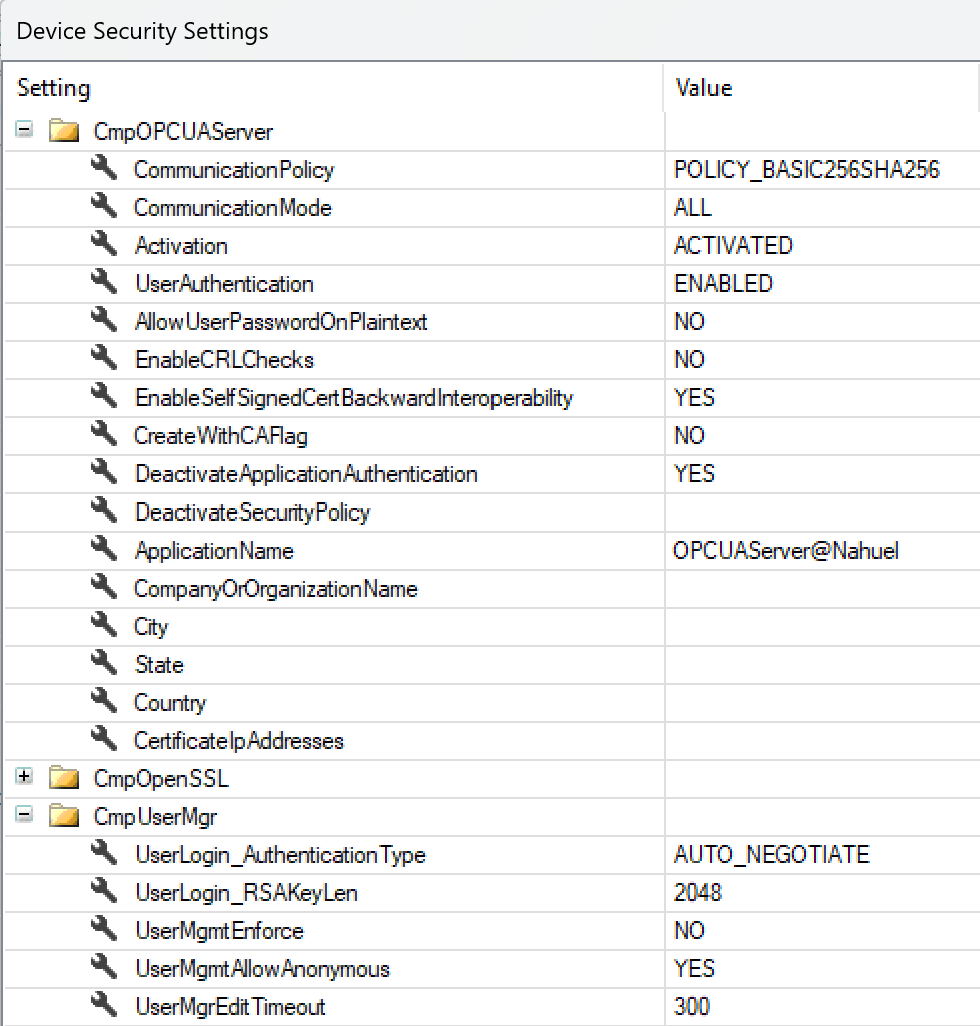
\includegraphics[width=0.7\textwidth]{config_OPC.png}
\end{figure}
También se desahabilitó el certificado de OPC-UA en Security Screen, y se movió a Trusted el certificado que genera Matlab al intentar conectarse por primera vez:
\begin{figure}[H]
    \centering
    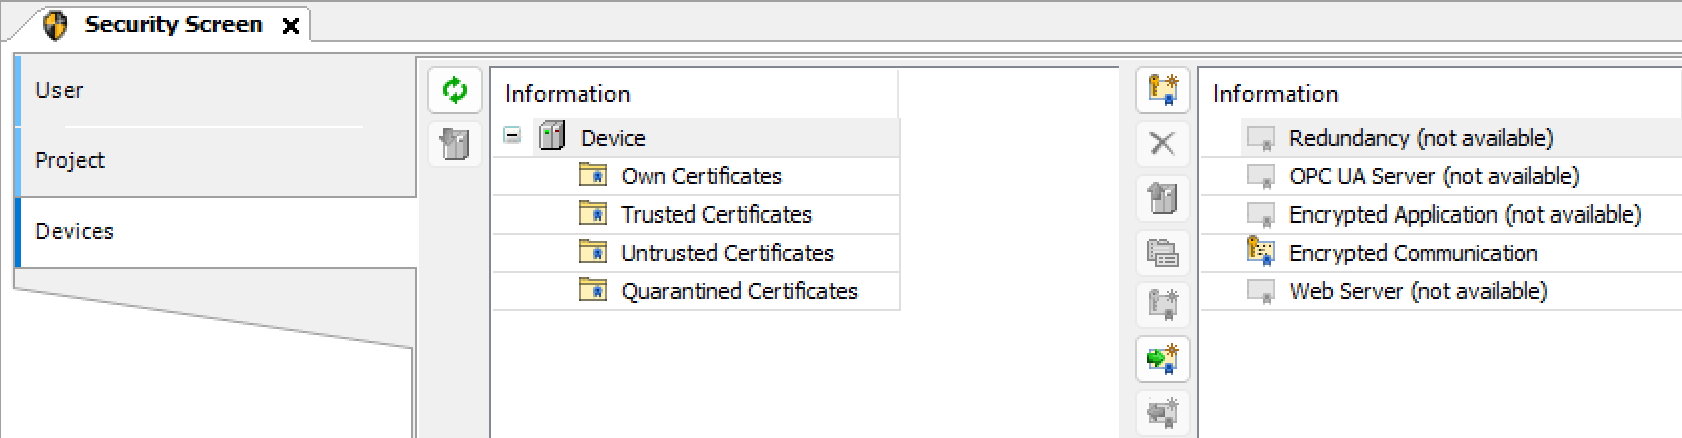
\includegraphics[width=1\textwidth]{config_OPC2.png}
\end{figure}
Estos ajustes permiten a Simulink conectarse al servidor OPC-UA de Codesys sin problemas, y leer/escribir las variables expuestas en tiempo real. Sin embargo, lo hace de forma anónima y sin seguridad alguna, lo cual no es recomendable para un entorno real, pero para fines de simulación y pruebas es suficiente.

Debido a la naturaleza de la comunicación OPC, cada lectura o escritura de una variable implica un proceso de comunicación cliente-servidor que introduce un retardo significativo. Este retardo se vuelve especialmente problemático cuando se intenta realizar lecturas/escrituras a alta frecuencia, lo cual es necesario para el control supervisor y más aún para el control regulatorio. OPC es un estandar de tipo TCP/IP, el cuál está diseñado para sistemas SCADA, con retardos de comunicación de $500$ ms o más, y no para sistemas de control en tiempo real. 

Para mitigar un poco este problema, se decidió implementar bloques de comunicación que se ejecuten a diferentes tiempos de muestreo. Esto enlentece la respuesta del modelo, causando delays peligrosos para la seguridad, pero permite que el sistema funcione de forma estable. El control regulatorio se ejecuta a $100$ ms, el control supervisor y de seguridad a $500$ ms. Para no tener errores con el heartbeat del watchdog, su variable corre al tiempo de muestro original de $20$ ms. De esta forma, se reduce la cantidad de lecturas/escrituras por segundo, disminuyendo la carga en la red y permitiendo Simulink pueda correr a $1$s por segundo de simulación.

Luego de algunas pruebas y reajustes, se mejoró significativamente la fluidez de la simulación, manteniendo una comunicación efectiva entre Simulink y Codesys. Y se ha podido comprobar de forma satisfactoria que el controlador responde de la misma manera que el modelado en Simulink.

A continuación, los bloques de escritura/lectura de las variables de control regulatorio, supervisor y seguridad, respectivamente:
\begin{figure}[H]
    \centering
    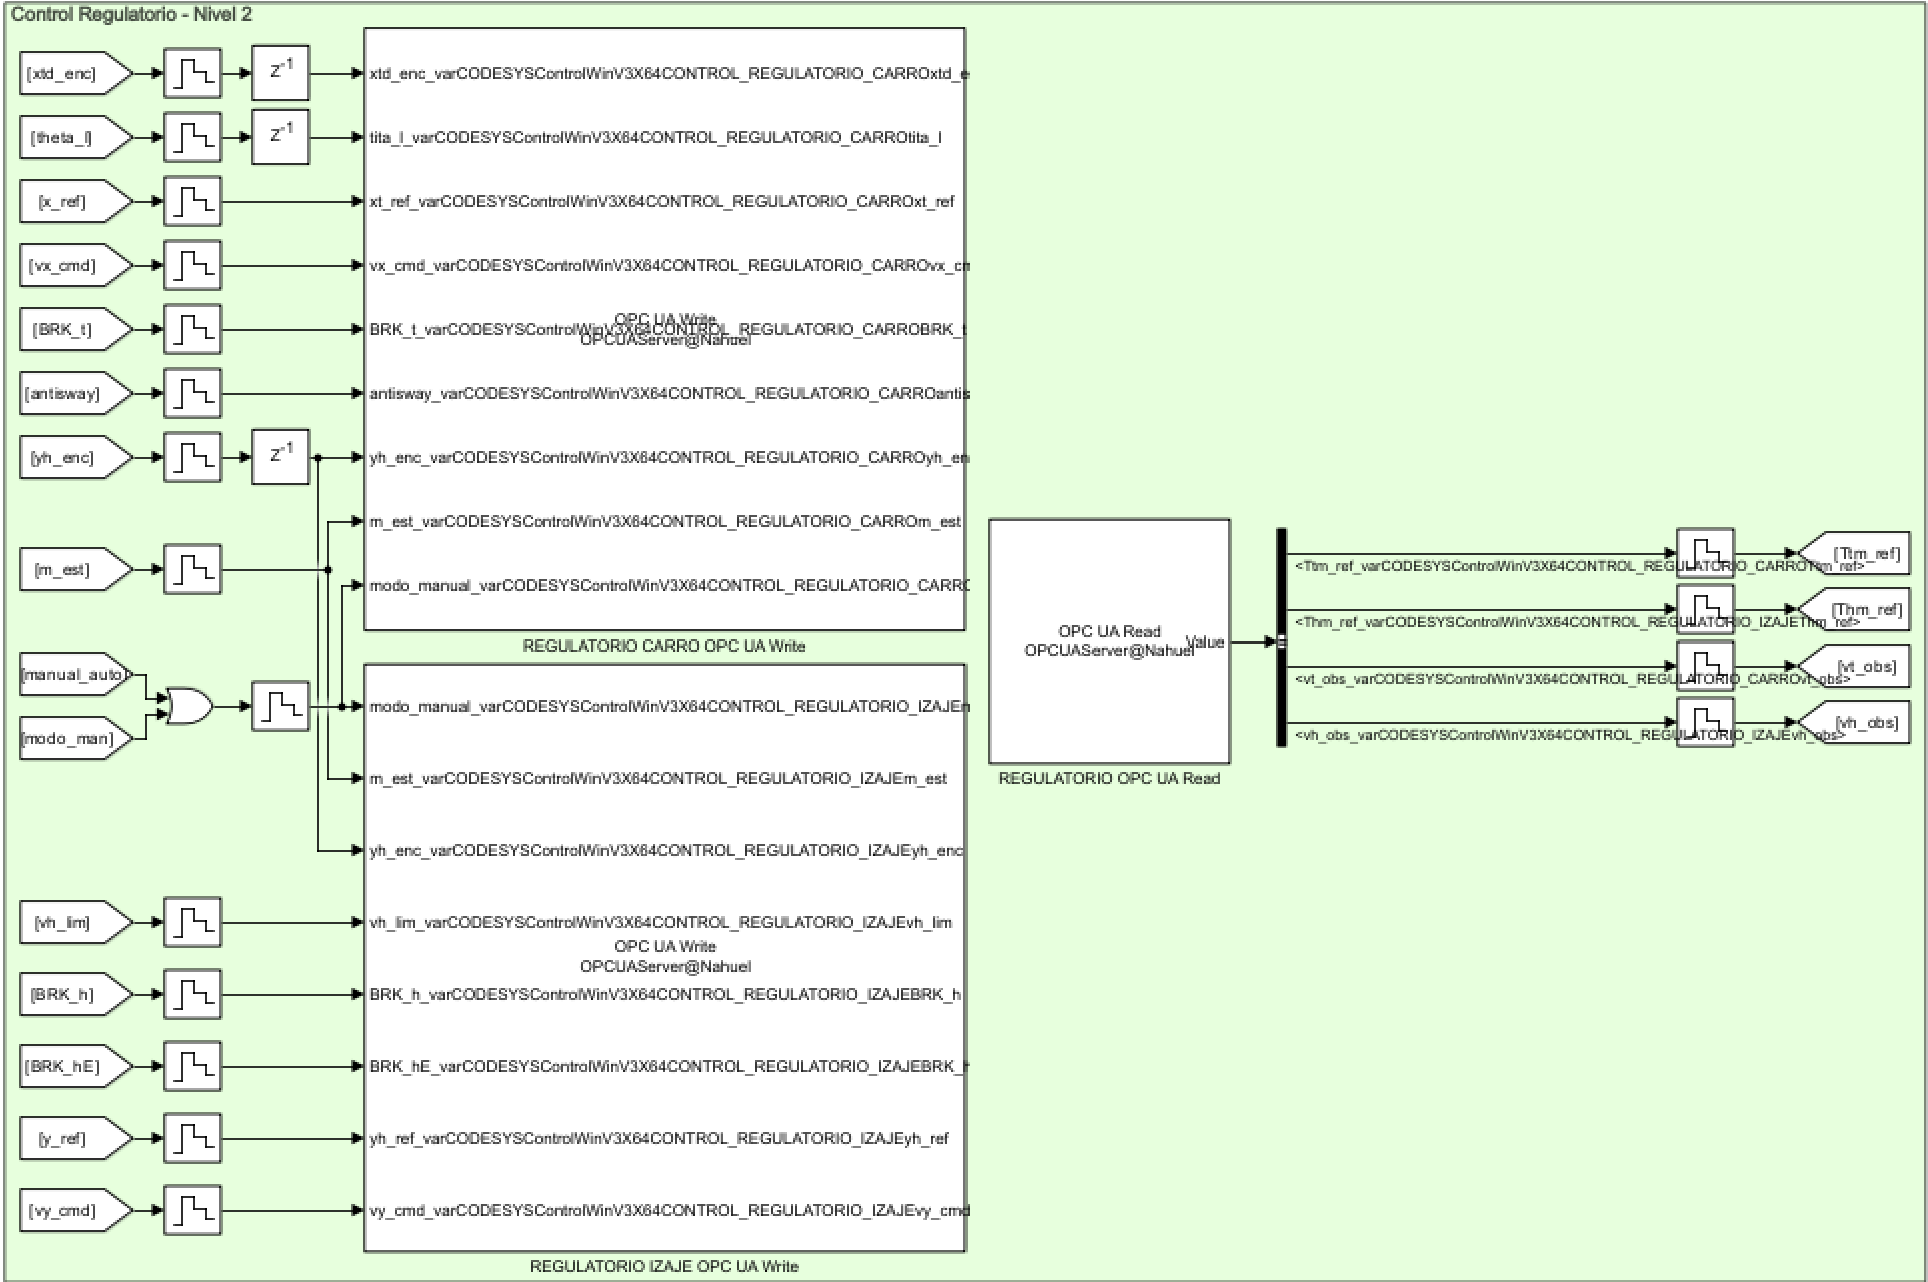
\includegraphics[width=1\textwidth]{simulink_client_regulatorio.png}
    \caption{Simulink - Cliente OPC-UA - Control Regulatorio.}
\end{figure}
\begin{figure}[H]
    \centering
    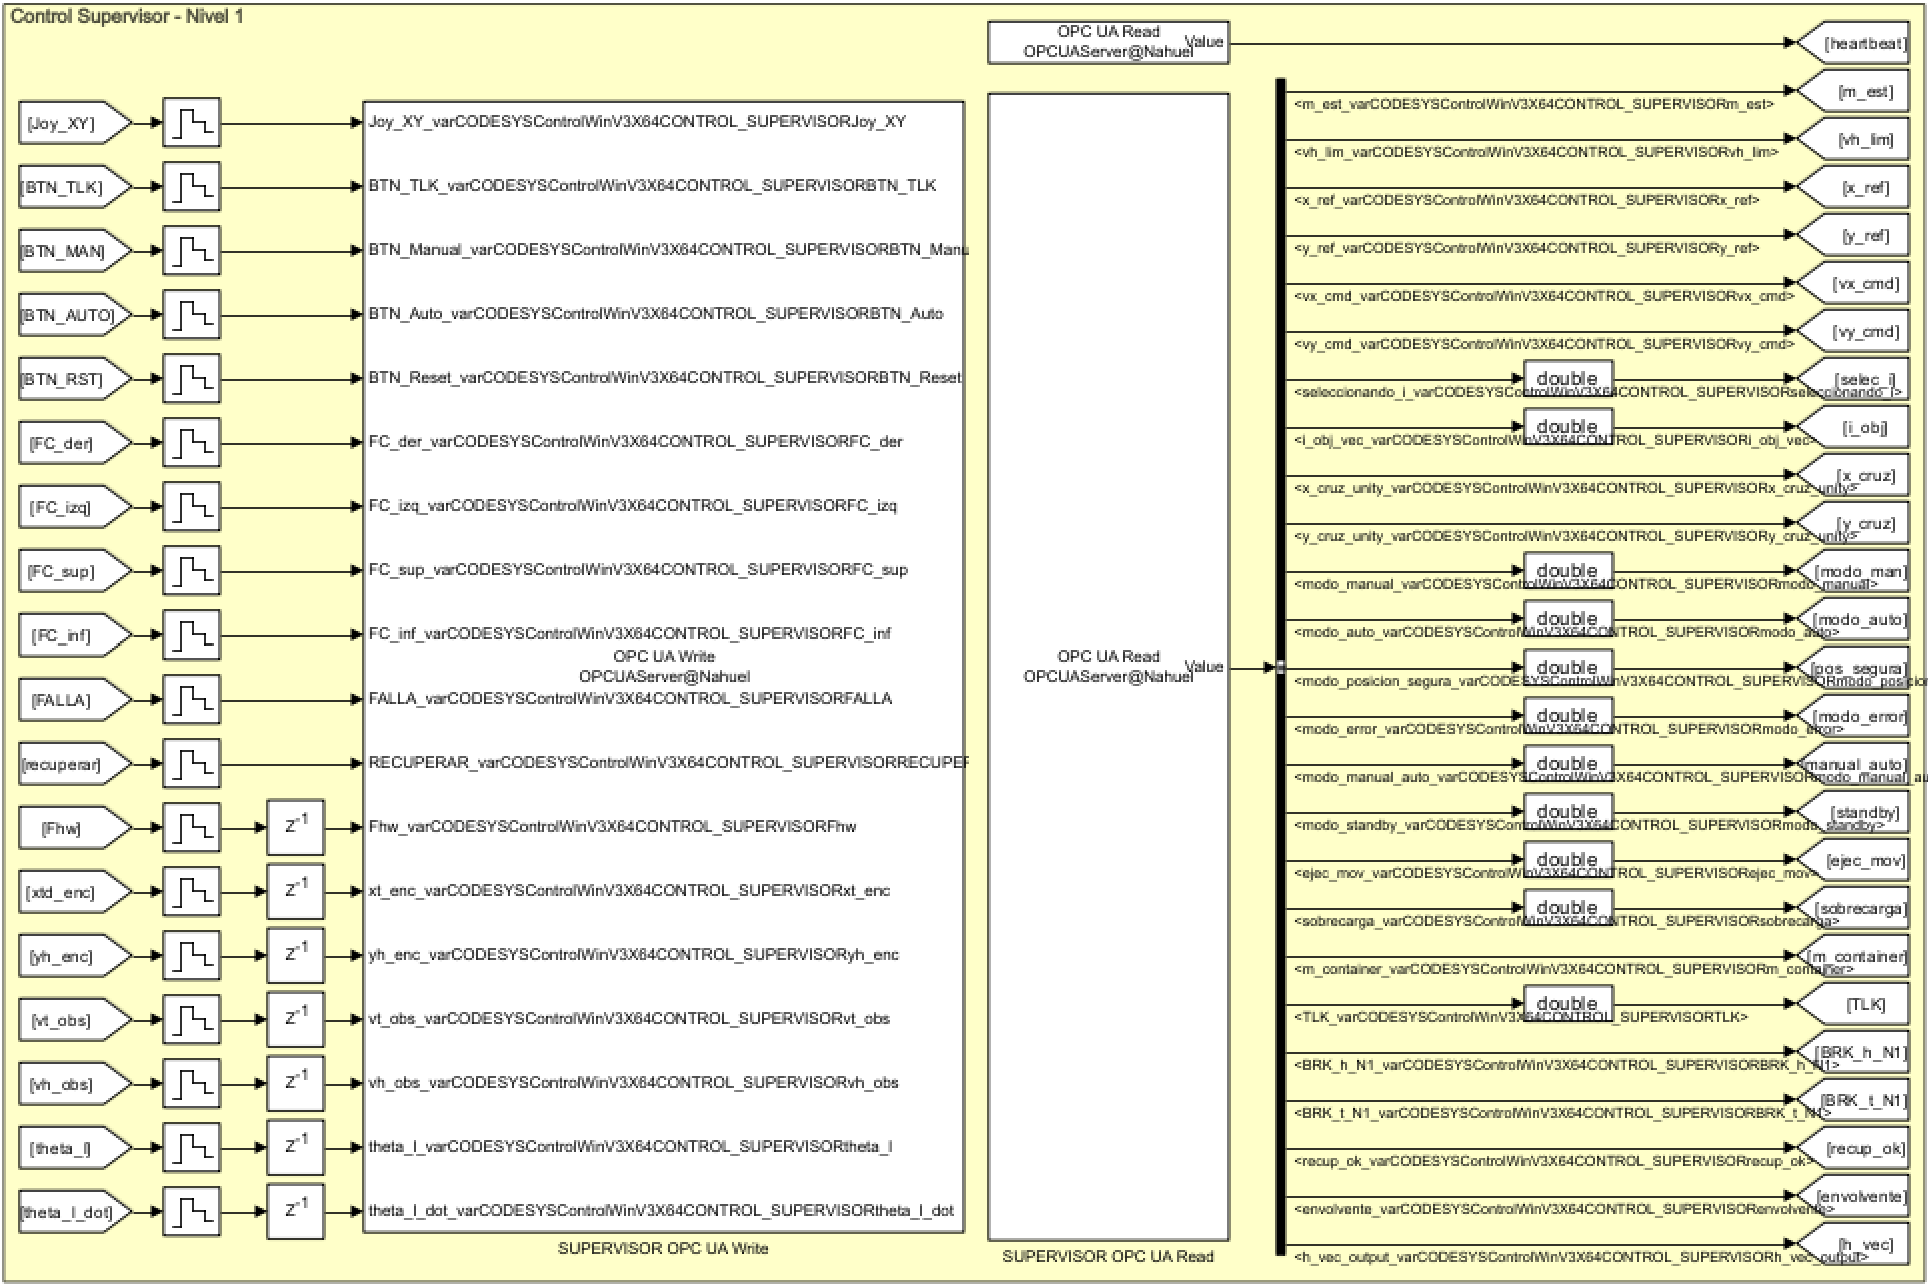
\includegraphics[width=1\textwidth]{simulink_client_supervisor.png}
    \caption{Simulink - Cliente OPC-UA - Control Supervisor.}
\end{figure}
\begin{figure}[H]
    \centering
    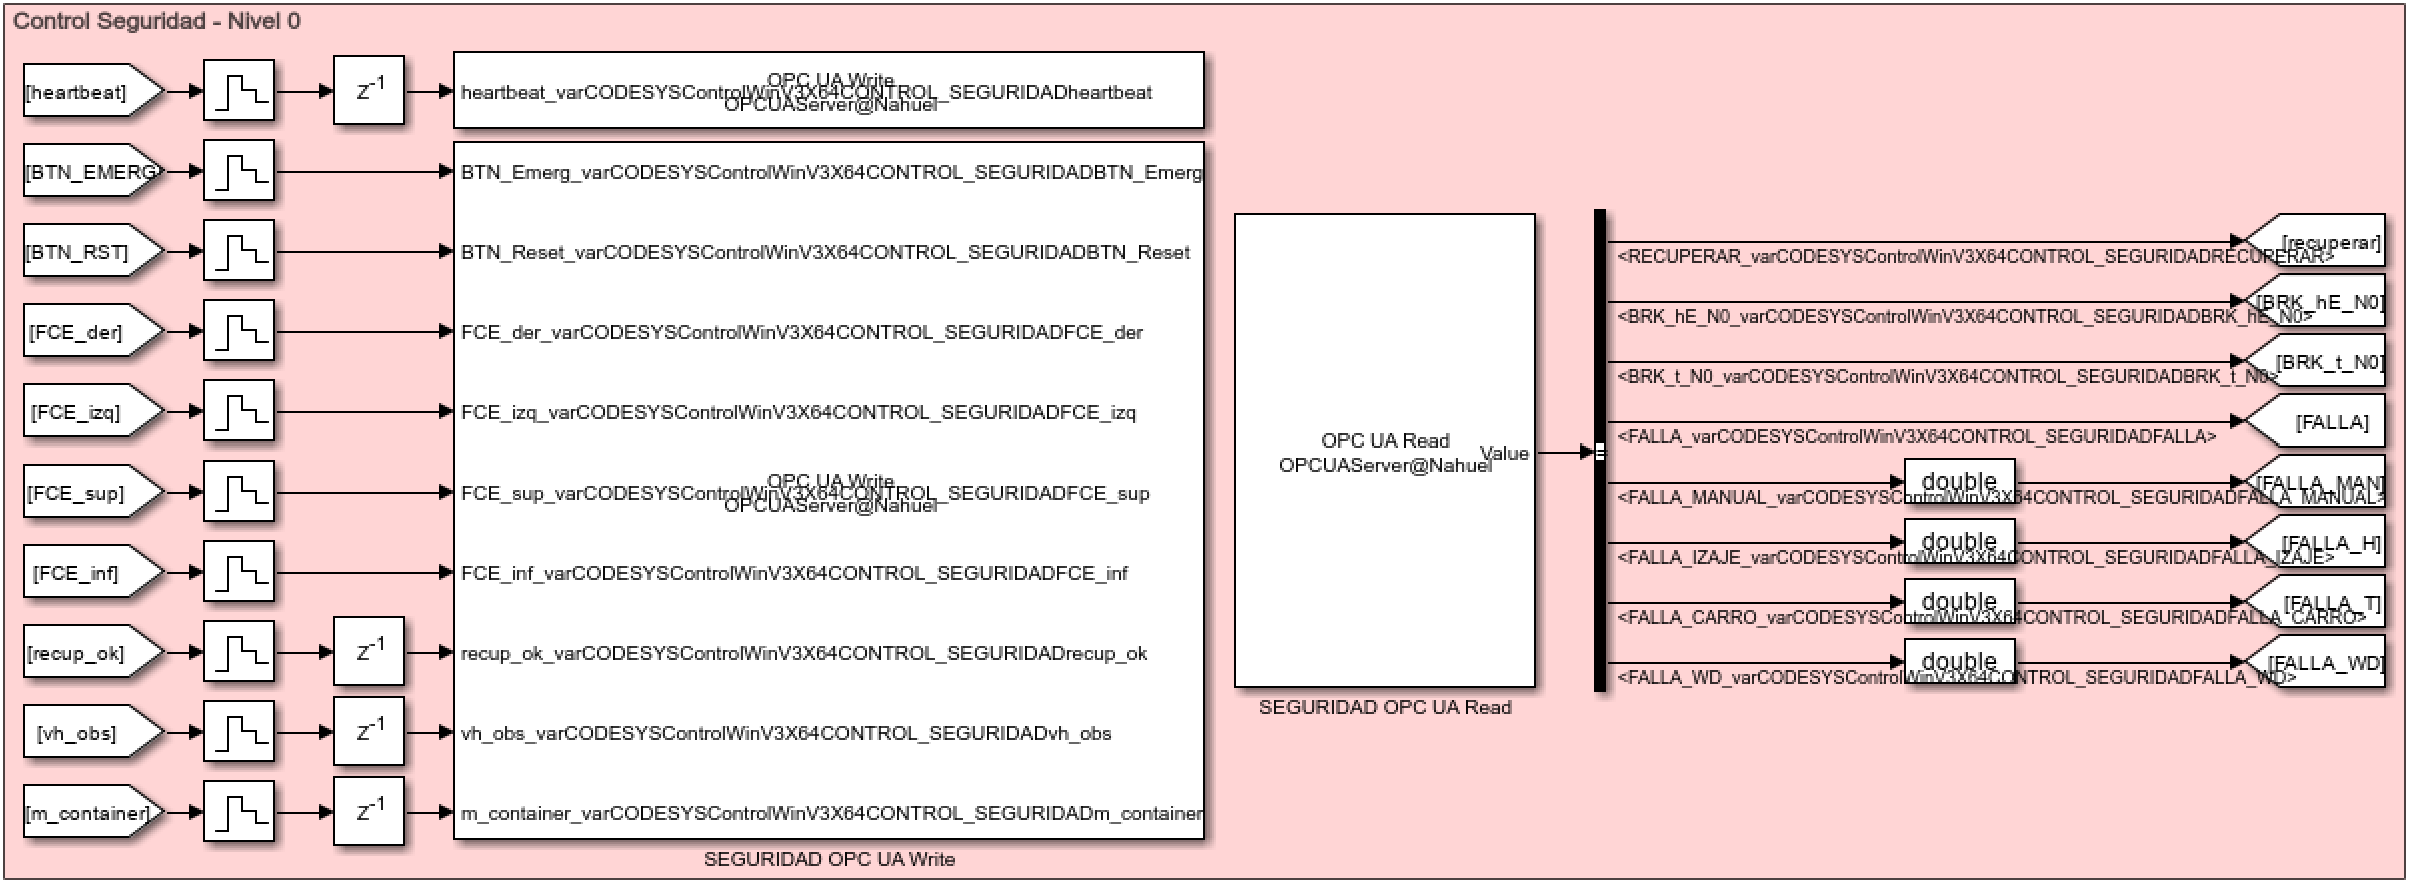
\includegraphics[width=1\textwidth]{simulink_client_seguridad.png}
    \caption{Simulink - Cliente OPC-UA - Control de Seguridad.}
\end{figure}

\section{Generación Automática de Código ST}
Simulink ofrece una herramienta llamada PLC Coder, que ofrece la capacidad de traducir automáticamente diagramas Stateflow a Texto Estructurado (ST) bajo la norma IEC 61131-3. Se procedió a analizar el código ST resultante de esta autogeneración. Se puede observar que el traductor implementa el autómata de forma ``plana'' y monolítica. Para lograrlo, recurre a una estructura de control \texttt{CASE} global que evalúa una variable entera representativa del estado actual, combinada con una densa red de sentencias \texttt{IF/ELSIF} anidadas para resolver las transiciones y acciones correspondientes.

A nivel de eficiencia computacional y carga de CPU, el rendimiento del código autogenerado es comparable al de una implementación manual. Los compiladores modernos de los PLC optimizan ambas estructuras a un código máquina de ejecución sumamente rápida, por lo que el tiempo de ciclo del autómata no se ve significativamente alterado por la elección de uno u otro método.

Sin embargo, la divergencia crítica entre ambos enfoques radica en la legibilidad, la mantenibilidad y el diagnóstico de fallas en el entorno industrial. El código ST autogenerado carece de trazabilidad visual; resulta ser una estructura de difícil interpretación para los operarios de planta. Por este motivo, en el proyecto se optó por utilizars solamente la traducción manual, utilizando SFC para la arquitectura general de los autómatas y reservando el Texto Estructurado exclusivamente para las acciones matemáticas subyacentes. 

Esta estrategia mantiene la potencia de cálculo del ST para las leyes de control cinemático, mientras que el entorno SFC proporciona un diagnóstico más visual. A continuación se muestran fragmentos del código autogenerado para el control de seguridad, evidenciando la complejidad y falta de claridad que presenta:
\begin{figure}[H]
    \centering
    \begin{subfigure}{0.85\textwidth}
        \centering
        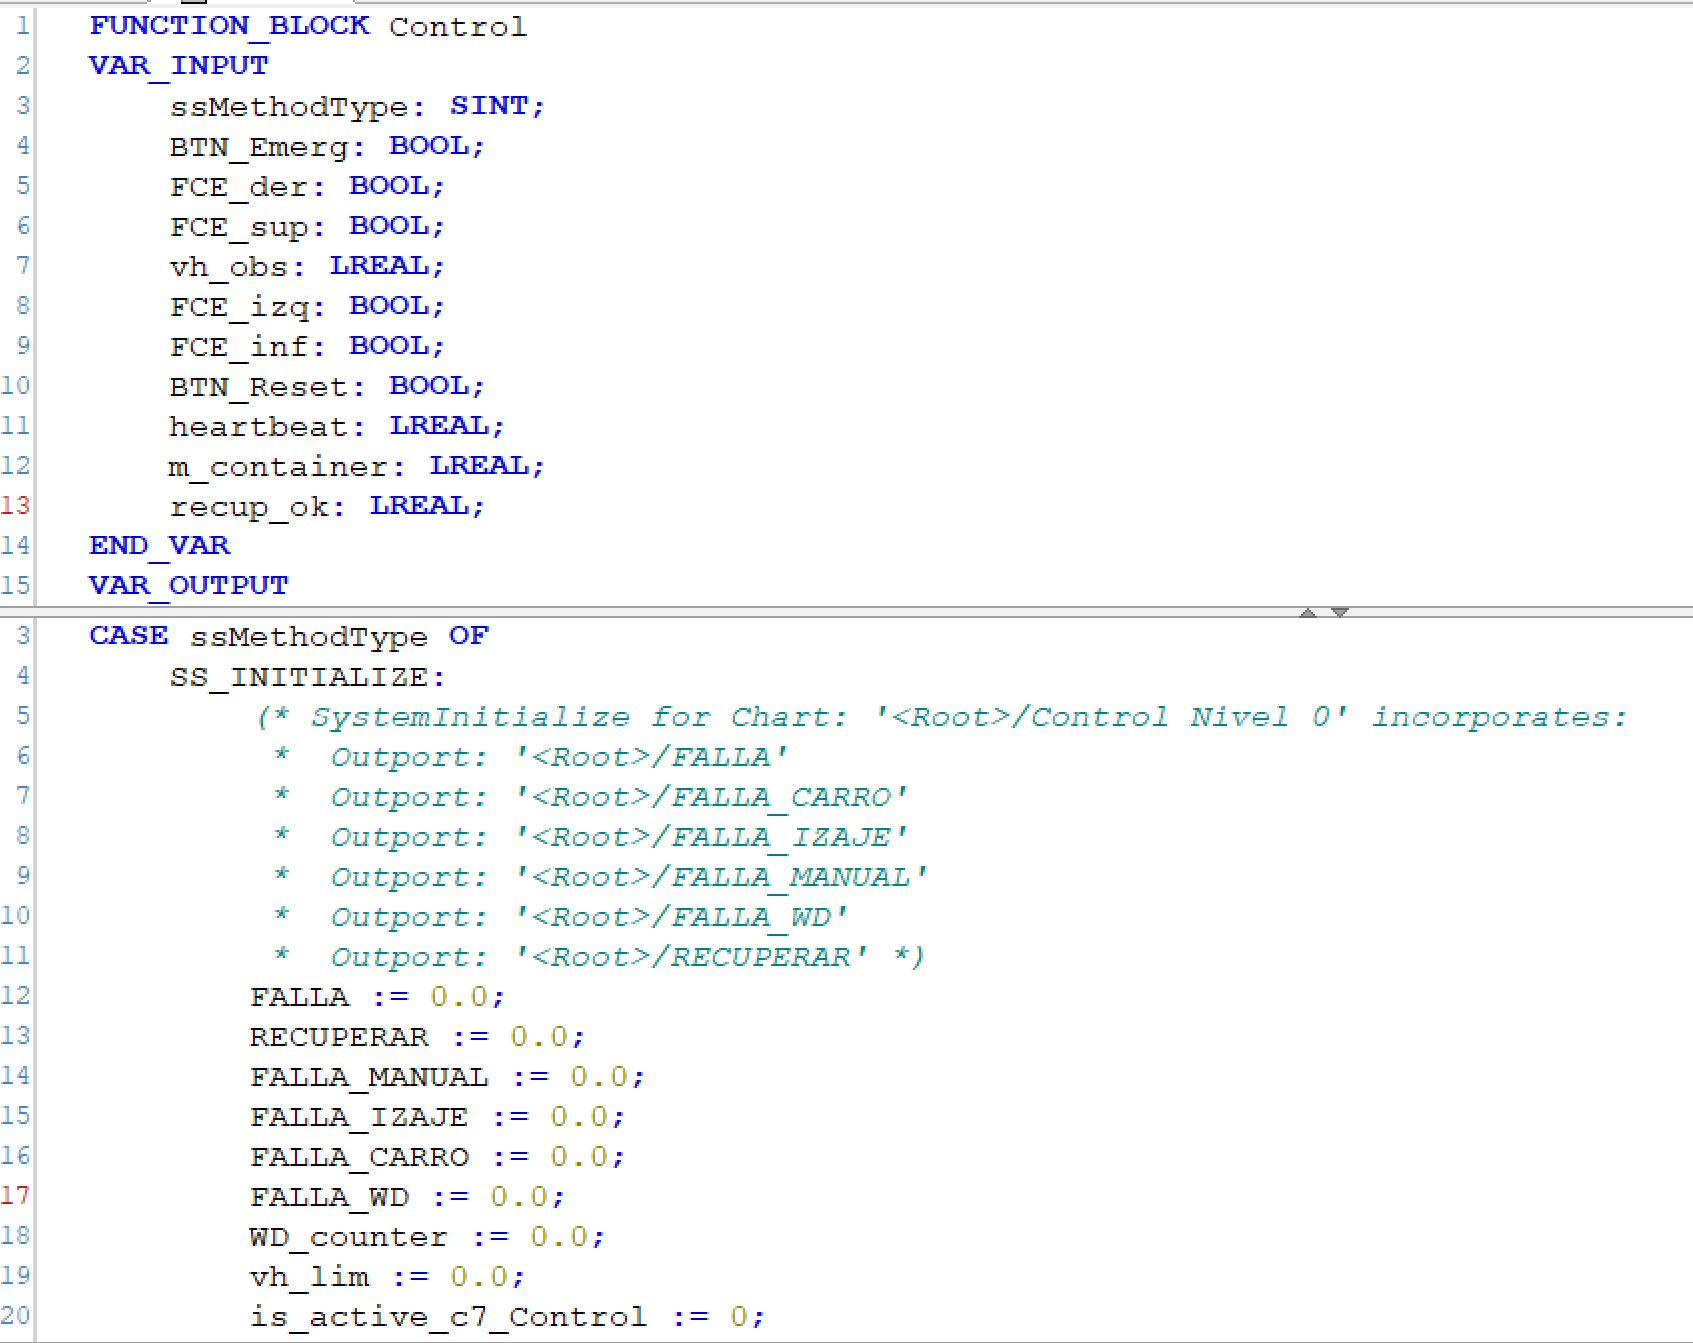
\includegraphics[width=\textwidth]{codigo_auto1.png}
    \end{subfigure}
    \begin{subfigure}{0.85\textwidth}
        \centering
        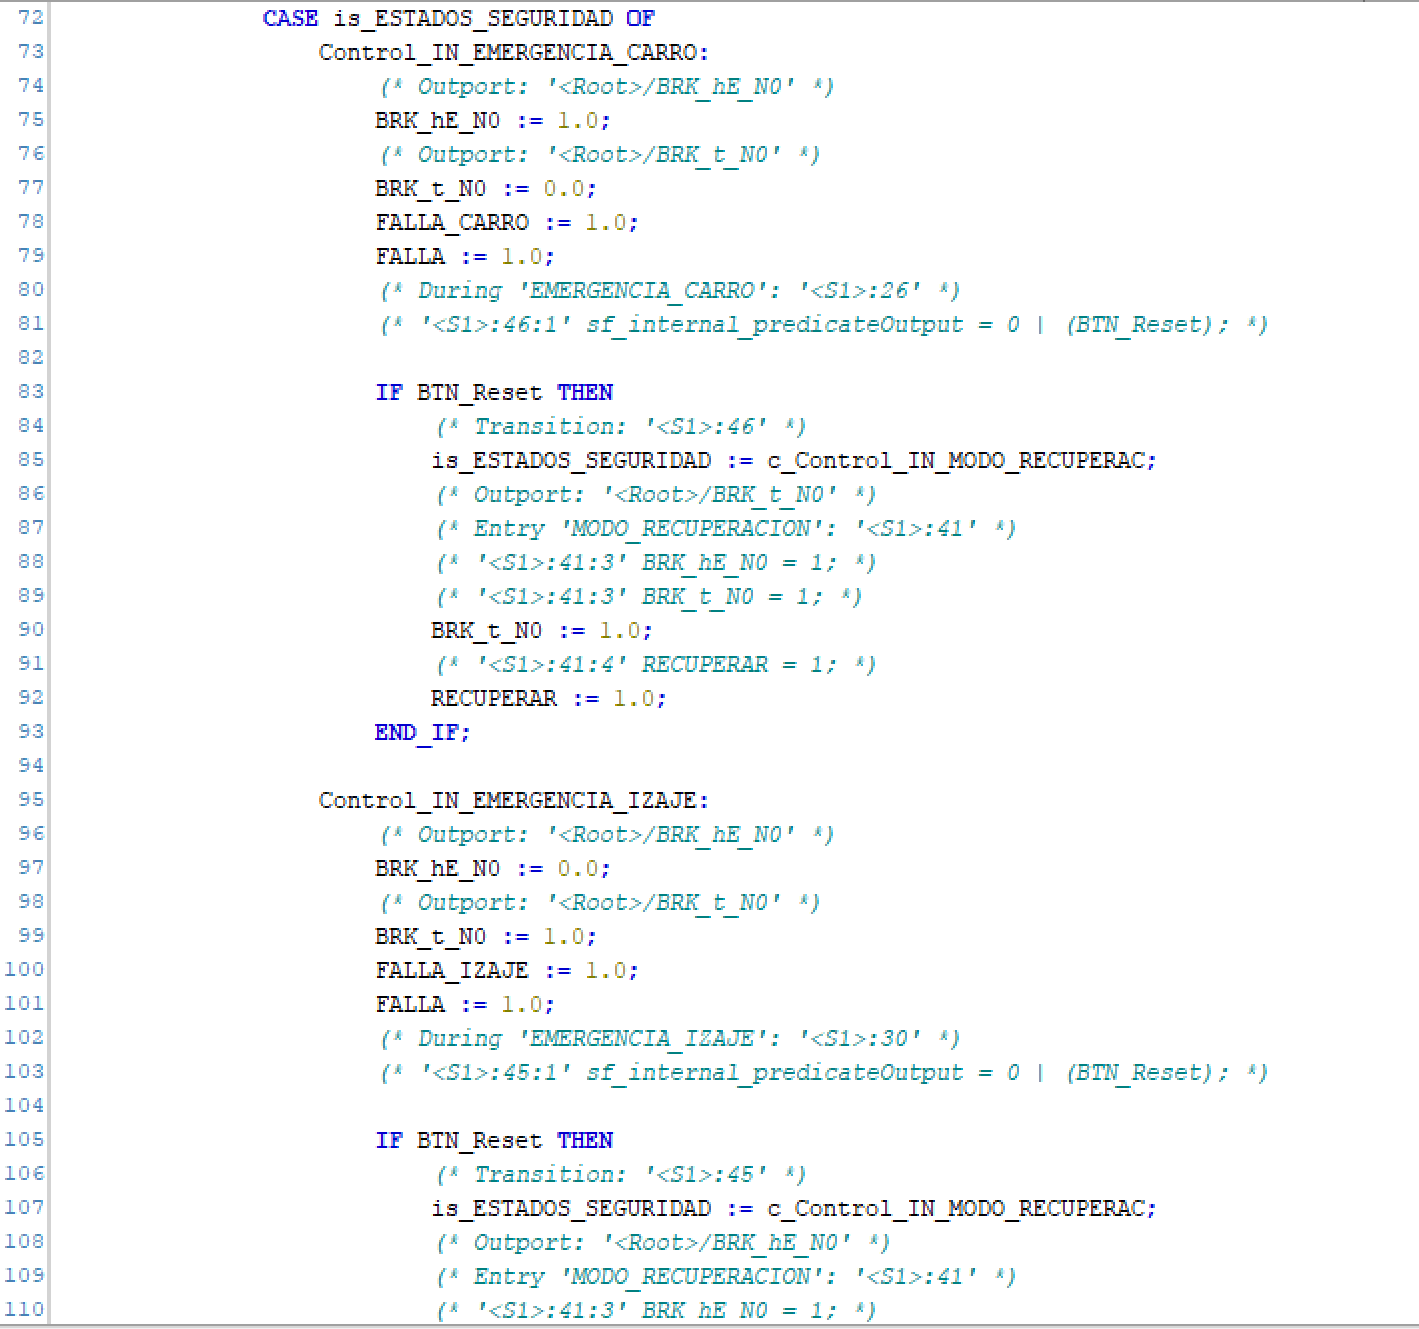
\includegraphics[width=\textwidth]{codigo_auto2.png}
    \end{subfigure}
    \caption{Código generado por PLC Coder - Fragmentos del control de seguridad.}
\end{figure}

\newpage
\section{Conclusiones}
En este proyecto se logró atravesar las diferentes etapas del diseño de control, desde la modelación física y el desarrollo de controladores en Simulink, hasta la implementación en Codesys y la integración con una aplicación de visualización en Unity. En ese sentido, fue un trabajo integral de control mecatrónico, porque no se quedó solo en la simulación ni solo en la programación del PLC, sino que conectó modelado, control, supervisión y validación visual dentro de un mismo flujo.

Uno de los aprendizajes más importantes fue el valor del modelo físico. Tener una base dinámica razonable permitió diseñar y ajustar mejor los controladores, pero también dejó claro que todo modelo tiene límites y simplificaciones. Considerar esas limitaciones desde el principio ayudó a interpretar mejor los resultados y a no asumir comportamientos ideales que después no se sostienen al pasar a una arquitectura industrial.

También fue clave el modelo de los controles, sobre todo por cómo se organizaron los distintos niveles. El uso de herramientas como las máquinas de estado permitió estructurar la lógica de forma más clara y robusta, facilitando la detección de condiciones de falla y la definición de respuestas seguras ante eventos críticos.

Un desafío concreto fue adaptar la lógica desarrollada en Stateflow al entorno de Codesys. Pasar de un enfoque gráfico basado en estados y transiciones a una implementación en SFC y ST exigió reordenar la lógica, cuidar el manejo de eventos y temporizaciones, y validar que el comportamiento final se mantuviera equivalente al del modelo original.

Por último, el desarrollo de la interfaz gráfica en Unity aportó una representación visual en tiempo real muy útil para validar el comportamiento global de la grúa. Esta etapa permitió además incorporar y comprender la comunicación UDP entre Simulink y Unity, incluyendo el empaquetado y tratamiento de datos.

\section{Repositorio y Video Demostrativo}
El proyecto completo, incluyendo los modelos de Simulink, el código en ST para Codesys y la aplicación de Unity, se encuentra disponible en el siguiente \href{https://github.com/nahuelpucciarelli/AyCD-Proyecto.git}{repositorio de GitHub}.

Además, se ha preparado un video demostrativo que muestra el funcionamiento de la grúa en diferentes modos de operación, destacando la interacción entre los niveles de control y la visualización en Unity. El video se puede acceder a través del siguiente \href{https://youtu.be/EwhYYALPttk?si=lQyfEXJ0O0OWh1-4}{enlace a Youtube}.

\newpage
\begin{thebibliography}{9}
\bibitem{matlab} MATLAB and Simulink. The MathWorks, Inc.
\bibitem{codesys} CODESYS - The Industry 4.0 Automation Software. 3S-Smart Software Solutions.
\bibitem{unity} Unity - Game Engine. Unity Technologies.
\bibitem{siemes} \href{https://assets.new.siemens.com/siemens/assets/api/uuid:e50a2d23-95fc-401a-8f4b-a6aec736a100/simocrane-sway-control-system-for-sts.pdf}{Simocrane Sway Control System for STS. Siemens.}
\bibitem{swaycontrol} \href{https://www.cmco.com/globalassets/case-studies/sway-control-technology/swaycontrolwhitepaper.pdf}{Sway Control Technology - White Paper. CMCO.}
\bibitem{swaycontrol2} \href{https://sci-hub.st/10.5545/sv-jme.2010.127}{Anti-sway System for Ship-to-Shore Cranes.}
\bibitem{swaycontrol3} \href{https://sci-hub.st/10.1109/ICIEAM.2018.8728750}{Crane Anti-Sway Control System with Sway Angle Feedback}
\end{thebibliography}

\end{document}
